% %% ----------------------------------------------------------------
%% Thesis.tex -- MAIN FILE (the one that you compile with LaTeX)
%% ---------------------------------------------------------------- 

% Set up the document
\documentclass[a4paper, 11pt, oneside]{Thesis}  % Use the "Thesis" style, based on the ECS Thesis style by Steve Gunn
\graphicspath{images/}  % Location of the graphics files 

% Include any extra LaTeX packages required
\usepackage[square, numbers, comma, sort&compress]{natbib}  % Use the "Natbib" style for the references in the Bibliography

\hypersetup{urlcolor=blue, colorlinks=true}  % Colours hyperlinks in blue, but this can be distracting if there are many links.

\usepackage[doipre={DOI:~}]{uri} % loads "url", if not already loaded

% new \oset macro:
\makeatletter
\newcommand{\oset}[3][0ex]{%
  \mathrel{\mathop{#3}\limits^{
    \vbox to#1{\kern-2\ex@
    \hbox{$\scriptstyle#2$}\vss}}}}
\makeatother

%% ----------------------------------------------------------------
\begin{document}
\frontmatter      % Begin Roman style (i, ii, iii, iv...) page numbering

\maketitle
%% ----------------------------------------------------------------

\setstretch{1.3}  % It is better to have smaller font and larger line spacing than the other way round

% Define the page headers using the FancyHdr package and set up for one-sided printing
\fancyhead{}  % Clears all page headers and footers
\rhead{\thepage}  % Sets the right side header to show the page number
\lhead{}  % Clears the left side page header

\pagestyle{fancy}  % Finally, use the "fancy" page style to implement the FancyHdr headers

%% ----------------------------------------------------------------

% The Abstract Page
\addtotoc{Abstract}  % Add the "Abstract" page entry to the Contents
\abstract{
\addtocontents{toc}{\vspace{1em}}  % Add a gap in the Contents, for aesthetics
blah\ldots

}

\clearpage  % Abstract ended, start a new page
%% ----------------------------------------------------------------

\setstretch{1.3}  % Reset the line-spacing to 1.3 for body text (if it has changed)

% The Acknowledgements page, for thanking everyone
\acknowledgements{
\addtocontents{toc}{\vspace{1em}}  % Add a gap in the Contents, for aesthetics

blah\ldots

}
\clearpage  % End of the Acknowledgements
%% ----------------------------------------------------------------

\pagestyle{fancy}  %The page style headers have been "empty" all this time, now use the "fancy" headers as defined before to bring them back


%% ----------------------------------------------------------------
\lhead{\emph{Contents}}  % Set the left side page header to "Contents"
\tableofcontents  % Write out the Table of Contents

%% ----------------------------------------------------------------

\mainmatter	  % Begin normal, numeric (1,2,3...) page numbering


% Include the chapters of the thesis, as separate files

\chapter{Introduction}
\lhead{\emph{Introduction}}
The term ``self-testing" was coined by Mayers and Yao in 2004 \cite{Mayers2003}. Their paper paved the way for the relatively new field at the forefront of quantum cryptography. The aim of self-testing is to acquire knowledge about the quantum properties of an adversarial input-output device from a minimal set of assumptions, by only interacting with the device classically, i.e.\ passing an input bitstring and receiving an output bitstring for each input-output cycle. The vast majority of self-testing protocols rely on Bell non-locality. As such, they assume that the device is a multipartite system that is split into space-like separated subsystems that are noncommunicating for the duration of one input-output cycle. The key observation giving rise to the notion of self-testing is that there exist Bell non-local correlations that are compatible only with an essentially unique quantum model, comprised of quantum state and measurement operators. Bell non-locality further certifies that the input-output correlations were not simulated by a hackable classical device. While
many technical tools have been developed to bound compatible quantum models for Bell-type self-testing scenarios, the prospect of certifying quantum properties of unipartite quantum system remains largely underexplored. A promising undertaking is to identify sets of assumptions that facilitate self-testing of a unipartite system, without using entanglement and Bell non-locality as relevant resources. Apart from providing insight into the geometry of quantum correlations for more general scenarios, the potential usefulness of such protocols lies in the fact that the no-communication assumption underlying conventional self-testing approaches is hard to implement in practice. The natural starting point we take on in this thesis is to study the role of Kochen-Specker contextuality as a resource for self-testing, as it can be seen as an extension of Bell non-locality to more general, unipartite scenarios. 

This thesis discusses and recasts previous results \cite{Bharti2019} that identify Kochen-Specker contextuality as a resource for self-testing to a general prepare-and-measure scenario. In particular, we propose a protocol based on Spekkens contextuality, discuss its features, and identify conditions that allow us to relax unphysical restrictions on measurement operators, imposed in \cite{Bharti2019}. Along the way, we characterize the resources in terms of memory needed by a pre-programmed classical device to simulate the optimal correlations to the protocol in \cite{Bharti2019}, and present an improved proof of robustness to noise.

The thesis is organized as follows:
In Section \ref{sec:kscontextuality}, we introduce the notion of Kochen-Specker contextuality, which aims to capture the way in which quantum mechanics deviates from our classical intuition, even for unipartite systems. We will derive a class of KS non-contextuality inequalities in Section \ref{sec:kcbs} that delimit classical from quantum correlations, analogously to Bell inequalities for multipartite systems. In Section \ref{sec:csw}, we introduce graph theoretic tools, proposed in \cite{Cabello2014}, that allow for a rigorous analysis of these KS non-contextuality inequalities. In particular, these tools enable us to identify and study optimal classical behaviours that saturate the non-contextual bounds, as well as optimal quantum models that produce maximal violations of the inequalities, relevant to self-testing. Section \ref{sec:self-testing} introduces the concept of self-testing in the context of multipartite Bell scenarios, which allows for powerful inferences about the quantum properties of a correlation experiment from minimal assumptions. Additionally, Section \ref{sec:self-testing} points out in what ways this concept can be modified to accommodate unipartite systems with no space-like separation. Equipped with the graph-theoretic tools presented in Section \ref{sec:csw}, we will demonstrate that the KS non-contextuality inequalities in \ref{sec:kcbs} facilitate noise-robust self-testing, as was proved in \cite{Bharti2019}, and improve the robustness to noise. Section \ref{sec:kcbs} also identifies the assumptions that go into this self-testing protocol. In particular, we find that one has to bound the information carrying capacity of the device to exclude the possibility of a pre-programmed classical computer generating the correlations. In an attempt to relax some of the unphysical constraints, such as the restriction to sharp measurements, we shift to a general prepare-and-measure scenario. Spekkens revised notion of non-contextuality, which will be introduced in Section \ref{sec:spekkcont}, is formulated within this general framework. Spekkens operational notion of contextuality will provide us with more suitable and robust tests of non-classicality.
Finally, in Section \ref{sec:protocols}, we submit a self-testing protocol based on Spekkens contextuality and discuss its merits and drawbacks, compared to the protocol in Section \ref{sec:contselftesting}.
\chapter{Kochen-Specker contextuality}
\label{sec:kscontextuality}
\lhead{\emph{Kochen-Specker contextuality}}
The Kochen-Specker (KS) Theorem \cite{Kochen1968} is the often overlooked brother of Bell's monumental no-go theorem \cite{Bell1964}. In loose terms, Bell's Theorem proves that quantum mechanics (QM) cannot be described in terms of a local hidden variable model (HVM). A ``Bell inequality" is a condition measurement correlations must obey, for reality to permit a local HVM description. Violations of Bell inequalities have been observed in numerous experiments: The well-known Delft experiment of 2015 was the first loophole-free confirmation of such violations \cite{Hensen2015}. As will be discussed in Section \ref{sec:bell}, Bell locality and KS non-contextuality are closely related, locality being the weaker assumption and justified by special relativity. Nevertheless, the KS Theorem has several distinct features that deserve to be studied in their own right. Most notably, KS contextuality allows one to examine how even single quantum systems are incompatible with a seemingly orthodox classical description in terms of hidden variables \cite{Pusey2019}. In contrast, Bell tests require two or more space-like separated quantum systems, in order for the measurement statistics to exhibit the characteristic Bell non-locality. The reason for this is that we observe violations of Bell inequalities for entangled quantum systems. An immediate consequence is that the notion of KS contextuality applies to a much broader class of experiments.

\section[Introductory example\\ Specker's three boxes]{Introductory example\\ \large{Specker's three boxes}}
\label{sec:threeboxes}
Section \ref{sec:kscont} will give a formal definition of KS non-contextuality. Nevertheless, we shall first consider a simple example that illustrates the concept. It is taken from Specker's 1960 paper “The logic of propositions which are not simultaneously decidable” \cite{Specker1975}, which also gives a nice accompanying parable about an overprotective seer that teaches at the school of prophets in the fictitious place Arba’ila. Fairy tales aside, consider three boxes, labelled with 1, 2, 3, that can each be in one of two states: empty or containing a gem. The state of a box can be measured by opening the lid and peeking inside. Let $M_{1}$, $M_{2}$, $M_{3}$ denote the three two-outcome measurements (with outcomes “empty” or “gem”) of the boxes. Further assume, rather unnaturally, that it is impossible to open all three boxes simultaneously. Rather, only pairs of boxes may be jointly measured. Figure \ref{fig:3boxes} depicts the setting of Specker's “three boxes” example. For some repeatable preparation of the system, one curiously observes the following: opening pairs of boxes always yields anti-correlated measurement outcomes (that is, one of the boxes will be empty and the other will contain a gem). How can these statistics be reconciled with a naive model of reality that assumes the three boxes to be in some underlying state that specifies their contents? As we can only ever open two boxes simultaneously, we can never observe this hidden state of reality. Importantly, a valid assignment of gems to the three boxes must be compatible with the observed anti-correlated outcomes. It turns out, as the reader should convince themself, that any assignment of gems to the boxes is incompatible with the observed statistics. Assuming that the pairs of boxes to be measured are picked at random, in a uniform way, the probability of observing anti-correlated outcomes is bounded by $p(\text{anti-correlated})\leqslant\frac{2}{3}$ and we conclude that the naive type of HVM we just considered is unable to account for the experimental data.

\begin{figure}
\centering
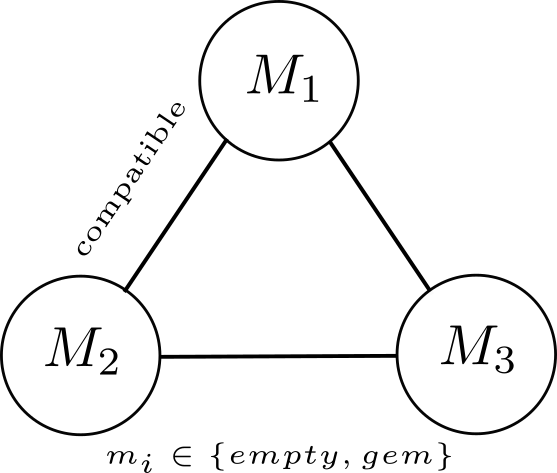
\includegraphics[width=0.4\textwidth]{images/3boxes.png}
\caption{Specker's ``three boxes" example. Three boxes 1,2,3 can each either hold a gem or be empty. The measurement $M_i$ corresponds to opening the lid of the $i$th box and checking its contents. The outcome of measurement $M_i$ is denoted by $m_i$. A solid line between measurements means that these are compatible and can be measured simultaneously. Despite all measurements being pairwise compatible, only pairs of boxes can be jointly measured. Measuring pairs of boxes always yields anti-correlated outcomes.}
\label{fig:3boxes}
\end{figure}

The point is that we have in fact considered a deterministic and non-contextual HVM to describe the three boxes. Deterministic just means that the underlying state of the system fixes all measurement outcomes and not just a probability distribution over possible outcomes. More interestingly, we define non-contextuality for the time being as the critical assumption that the outcome of some measurement should be the same, regardless of which other compatible\footnote{Two measurements are called \emph{compatible} if they can be performed simultaneously. While this ``definition" is sufficient for now, we will refine it in Section \ref{sec:correxp}.} measurement is performed simultaneously. Allowing the outcome of a measurement to depend on what other compatible measurement is performed together with it, could indeed account for the observed correlations.

\section{The Kochen-Specker Theorem, informally}
Informally, the KS Theorem states the following:

\begin{theorem}[Kochen-Specker, informal]
A non-contextual deterministic HVM of QM for Hilbert spaces of dimension $\geq3$ is impossible.
\end{theorem}

It is tempting to try to recast Specker's “three boxes” example to the realm of quantum theory. Within the theory of QM, compatible measurements are conventionally represented by commuting Hermitian operators. To implement the example in QM, we would have to find a quantum state $|\Psi\rangle$ and pairwise commuting two-outcome measurements $M_{1}$, $M_{2}$, $M_{3}$ not all simultaneously measurable, such that QM predicts $p(\text{anti-correlated})>\frac{2}{3}$. For the same reasons, this would imply that non-contextual deterministic HVM are not compatible with the predictions of QM and would prove the KS Theorem, albeit initially only for a fixed dimension that may be greater than 3. However, if all three measurements are pairwise commuting, they necessarily have a joint eigenbasis. Thus, all three measurements could be simultaneously performed and correlations with $p(\text{success})>\frac{2}{3}$ could not arise. Despite this, Sections \ref{sec:formalproof}, \ref{sec:4dim} feature examples that are similar in spirit, if a little more involved, and which can indeed be implemented by QM.

Specker hypothesized pairwise compatibility implying global compatibility to be the ``fundamental theorem of QM" that shapes the set of quantum correlations \cite{Cabello2012}. This is supported by the fact that for many correlation experiments the ``theorem" singles out correlations that are compatible with QM (and projective measurements) and offers an explanation for why quantum correlations cannot exceed certain mystifying bounds we will encounter in Section \ref{sec:cswhierarch} \cite{Cabello2013}.

Before we can discuss the KS Theorem and its proof in formal terms, as is done in Section \ref{sec:formalproof}, we will begin by establishing a general mathematical framework of HVM in Section \ref{sec:hvm}. Section \ref{sec:mnts} introduces two ways of representing measurements in QM, leading to two equivalent notions of KS non-contextuality, as defined in Section \ref{sec:kscont}. Section \ref{sec:4dim} presents a considerably simpler proof of the KS Theorem that holds for four-dimensional systems. The connection between KS non-contextuality and local causality will be the subject of Section \ref{sec:bell}, highlighting the similarities and differences between the KS Theorem and Bell's Theorem. This discussion will point out several flaws of the traditional notion of KS contextuality and addresses the need for an operational notion. A proposal of that sort by Spekkens will be introduced later in Section \ref{sec:spekkcont}. Finally, in Section \ref{sec:kcbs} we will discuss an important class of KS contextuality experiments involving a qutrit, namely the KCBS scenario and generalizations of it. For these experiments one can derive KS non-contextuality inequalities on the convex set of possible correlations, analogously to Bell inequalities, that must hold for all non-contextual behaviours. Interestingly, these inequalities turn out to be incompatible with the predictions of QM for some quantum states.

\section{General framework of hidden variable models}
\label{sec:hvm}
An ontological model of QM\footnote{The following applies more generally for ontological models of arbitrary operational theories. An operational theory is one that makes testable predictions.}, more commonly referred to as a hidden variable model (HVM), presupposes some ontic state space $\Lambda$. An ontic state $\lambda\in\Lambda$ is a state of reality or “matter of fact” description of the system. It holds all attributes of the system, regardless of whether they are known or even knowable (hence hidden variables). Importantly, a HVM posits that our system is at each time point in some ontic state with corresponding definite attributes, even when these are not being subjected to measurements. In the case of KS contextuality we will only consider \textbf{deterministic} HVM, meaning that an ontic state fixes the outcomes of all possible measurements that may be performed on the system. Uncertainty in the ontic state that was prepared results in a probabilistic distribution of measurement outcomes. It is helpful to formalize this and boil the assumptions down to a simple mathematical model. We follow the notation and terminology of \cite{Spekkens2005} 

With any preparations $P$ one can associate a probability density function $\mu_{P}(\lambda)$ on the ontic state space $\Lambda$. One can think of a preparation as an ensemble of systems, much like in the spirit of statistical mechanics, whereby each individual member of the ensemble is in some well-defined ontic state $\lambda\in\Lambda$. The probability of picking a system from the ensemble at random with a hidden parameter contained in some region $\mathcal{A}\subset\Lambda$, is then given by $\int_{\mathcal{A}}\mu_{P}(\lambda)d\lambda$. By normalization, we require that $\int_{\Lambda}\mu_{P}(\lambda)d\lambda=1$.

Measurements $M$ can be associated with sets of indicator functions $\left\{ \xi_{M,k}\right\} _{k}$ on $\Lambda$, one for each measurement outcome $k$. The value $\xi_{M,k}(\lambda)\in\{0,1\}$ is the conditional probability of the measurement $M$ yielding the outcome $k$, given that the system is in the ontic state $\lambda$. Since we are considering only deterministic HVM, meaning that the ontic state of the system fixes all measurement outcomes with certainty, this conditional probability must be either 0 or 1. Naturally, the indicator functions for the different measurement outcomes must obey $\sum_{k}\xi_{M,k}(\lambda)=1$ $\forall\lambda\in\Lambda$. Section \ref{sec:mnts} will introduce two ways of representing measurements in QM. We will apply the framework introduced in this section to these, in order to treat quantum measurements within HVM. Lastly, for the HVM to be consistent with the testable predictions of the operational theory it should model, it must hold that: $p(k\vert P,M)=\int_{\Lambda}d\lambda\thinspace\xi_{M,k}(\lambda)\mu_{P}(\lambda)$, where $p(k\vert P,M)$ describes the probability of observing the measurement outcome $k$, given measurement $M$ and preparation $P$, as proposed by the operational theory. The above quantities are pictorally summarized in Figure \ref{fig:hvm}, for the case of a two-outcome measurement $M$. In the following, when making reference to an arbitrary deterministic HVM of QM, we will implicitly assume an underlying ontic state space $\Lambda$ and indicator functions $\{\xi_{M,k}\}_{k}$ for all measurements $M$ with possible outcomes $k$.

\begin{figure}
    \centering
    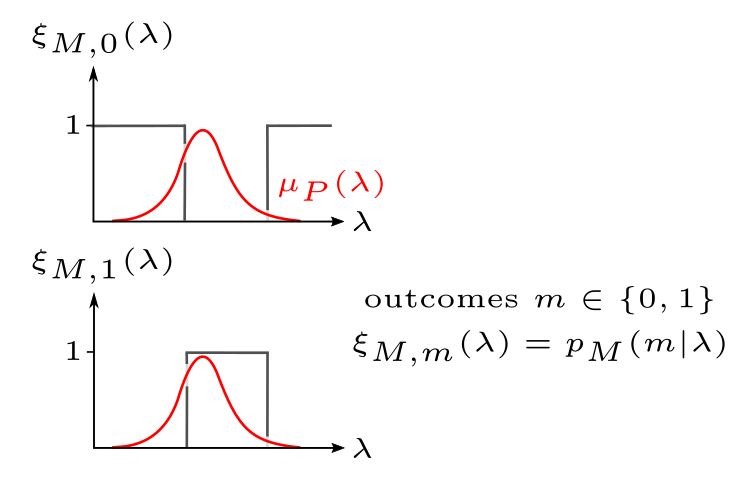
\includegraphics[width=0.7\textwidth]{images/hvm.png}
    \caption{Summary of the constituents characterizing a deterministic HVM for the case of a two-outcome measurement.\hfill\break A system's ontic state space $\Lambda$, here depicted as a one-dimensional axis, comprises all possible states of reality. A state preparation $P$ can be associated with a probability density function on $\Lambda$, modelling the uncertainty in the prepared ontic state. A deterministic HVM associates with any measurement $M$, here a two-outcome measurement with outcomes $m\in\{0,1\}$, a set of indicator functions $\{\xi_{M,m}\}_m$. The indicator function to measurement outcome $m$, $\xi_{M,m}:\Lambda\rightarrow\{0,1\}$, maps each ontic state to the probability of observing outcome $m$, conditioned on the system being in that ontic state.}
    \label{fig:hvm}
\end{figure}

\section{Measurements in quantum mechanics}
\label{sec:mnts}
Section \ref{sec:kscont} will define the notion of KS non-contextuality that is at the heart of the KS Theorem. It is an assumption about the type of HVM the theorem rules out and, in loose terms, pertains to the measurements within such a HVM. To set the stage for discussing KS non-contextuality, this section introduces two ways of representing (projective) measurements in QM. As will be proved in Section \ref{sec:kscont}, the two notions of measurements will give us two equivalent notions of KS non-contextuality, each of which will be particularly useful for certain purposes. Note that within the framework of KS contextuality we assume all quantum measurements to be projective. On the other hand, in quantum information theory a general quantum measurement is given by a set of positive semi-definite operators whose sum is the identity, a so-called positive operator valued measure (POVM) \cite{Nielsen2010}. A projective measurement, or projection-valued measure (PVM), is also a POVM, however the reverse generally does not hold. The two are related in the sense that every POVM can be seen as a PVM acting on an extended Hilbert space, followed by us discarding some degrees of freedom, a consequence of Naimark's dilation theorem \cite{Watrous2018}. Thus, assuming all quantum measurements to be projective is in principle consistent with the existence of POVMs. In Section \ref{sec:spekkcont}, we present a revision of the traditional notion of KS contextuality due to Spekkens. Spekkens contextuality is defined largely in terms of operational primitives and is able to accommodate more general POVM quantum measurements. As physical measurements are non-ideal, we must account for these in view of our goal to certify quantum properties of a single quantum device under operational assumptions.

The conventional way of representing projective measurements in QM is in terms of Hermitian operators, with every measurement being relatable to a set of pairwise commuting and thus simultaneously measurable operators that share a common eigenbasis. Measurement outcomes are tuples of simultaneous eigenvalues. The spectrum of a Hermitian operator A is denoted by $\sigma(A)$ and the set of all Hermitian operators on a Hilbert space $\mathcal{H}$ is denoted by $\operatorname{Herm}(\mathcal{H})$. 

\begin{definition}
\label{def:projmntsherm}
Let $\mathcal{H}$ be the system Hilbert space.\hfill\break A \emph{projective quantum measurement} $\mathcal{M}=(X_{1},X_{2},\dots)\subset\operatorname{Herm}(\mathcal{H})$ is an ordered set of pairwise commuting Hermitian operators.\hfill\break An \emph{outcome of a projective quantum measurement} $\mathcal{M}$ is a tuple\hfill\break 
$\left(x_{1},x_{2},\dots\right)\in\bigtimes_{X_{i}\in\mathcal{M}}\sigma(X_{i})$ of simultaneous eigenvalues to operators in $\mathcal{M}$, meaning that there exists a common eigenvector $\ket{\Psi} \in\mathcal{H}\backslash\{0\}$ with $X_{k}\ket{\Psi} =x_{k}\ket{\Psi}$  $\forall X_{k}\in\mathcal{M}$.
\end{definition}

An ordered set of commuting Hermitian operators like in \ref{def:projmntsherm} is also referred to as a ``measurement context". We say that $X_1$ is measured in the context $\mathcal{M}$. An example of a quantum measurement in this sense is given by “Pauli strings” on the composite Hilbert space $\mathbb{\mathbb{C}}^{2}\otimes\mathbb{C}^{2}$, for example
\begin{equation*}
\mathcal{M} =(\sigma_{x}^{1} \coloneqq \sigma_{x}\otimes
\mathbb{1},\thinspace\sigma_{x}^{2}\coloneqq\mathbb{1}\otimes\sigma_{x},\thinspace\sigma_{x}^{1}\sigma_{x}^{2}\coloneqq\sigma_{x}\otimes\sigma_{x})
\end{equation*} with outcomes
\begin{equation*}
\left\{ (1,1,1),(1,-1,-1),(-1,1,-1),(-1,-1,1)\right\}.
\end{equation*}
Each of the four outcome tuples corresponds to one of the four joint eigenstates that together span the four-dimensional Hilbert space. Additionally, each outcome tuple contains three values, corresponding to the three pairwise commuting Hermitian operators that constitute the measurement $\mathcal{M}$. We will revisit operators of this form in Section \ref{sec:4dim}, when discussing a simple, algebraic proof of the KS Theorem for four-dimensional Hilbert spaces.

Let us now apply the framework proposed in Section \ref{sec:hvm} to projective quantum measurements like in Defintion \ref{def:projmntsherm}. Let $A,B$ be two commuting Hermitian operators. If we assume the ontic state $\lambda\in\Lambda$ to be fixed, $\xi_{(A,B),(a,b)}(\lambda)$ describes a joint probability distribution $P_{\mathcal{A}\mathcal{B}}^{\lambda}(a,b)=\xi_{(A,B),(a,b)}(\lambda)$ for random variables $\mathcal{A},\mathcal{B}$, that hold eigenvalues of $A,B$, respectively.\hfill\break $P_{\mathcal{A}\mathcal{B}}^{\lambda}(a,b)$ gives the probability of obtaining outcome $(a,b)$ when performing the joint measurement $(A,B)$, conditioned on the system being in the ontic state $\lambda$. We can go from a joint probability distribution $P_{\mathcal{A}\mathcal{B}}^{\lambda}$ to the “marginal” distribution $P_{\mathcal{A}}^{\lambda}$ for random variable $\mathcal{A}$, by summing over all $b\in\sigma(B)$: $\sum_{b\in\sigma(B)}P_{\mathcal{A}\mathcal{B}}^{\lambda}(a,b)=P_{\mathcal{A}}^{\lambda}(a)$. We will revisit marginals of joint outcome probability distributions when defining the notion of KS non-contextuality in Section \ref{sec:kscont}.

An alternative way of representing measurements in QM is motivated by the spectral decomposition of Hermitian operators. It defines projective quantum measurements in terms of rays in a projective Hilbert space $\mathcal{P}(\mathcal{H})$. The projective Hilbert space $\mathcal{P}(\mathcal{H})$ of a complex Hilbert space $\mathcal{H}$ is defined as the set of equivalence classes $\{[\thinspace\ket{\Psi}\thinspace]\}_{\ket{\Psi} \in\mathcal{H}\backslash\{0\}}$ with respect to the equivalence relation $\ket{\Psi}\sim\ket{\Phi} \mathrel{\vcentcolon\Leftrightarrow}\exists\alpha\in\mathbb{C\backslash}\{0\}\vcentcolon\ket{\Psi} =\alpha\ket{\Phi}$. The equivalence classes of $\mathcal{P}(\mathcal{H})$ are called ``rays". Intuitively, one can think of $\mathcal{P}(H)$ as the ``unit sphere” of normalized vectors in $\mathcal{H}$, with every $\mathcal{H}\ni\ket{\Psi}\neq0$ being identified with its normalized counterpart. In this picture, a measurement can be specified by an orthonormal basis (ONB) $\{\ket{\Psi_{i}} \}_{i}$ of the Hilbert space, with measurement outcomes being represented by rays.

\begin{definition}
\label{def:projmntsbasis}
Let $\mathcal{H}$ be the system Hilbert space.\hfill\break
A \emph{projective quantum measurement with respect to a basis} $\mathcal{M}=\{\ket{\Psi_{i}} \}_{i}\subset\mathcal{\mathcal{P}}(\mathcal{H})$ is an ONB of $\mathcal{H}$. An \emph{outcome} of such a measurement $\mathcal{M}$ is a ray $\ket{\Psi_{k}} \in\mathcal{M}$.
\end{definition}

As will be discussed in the next section, an ONB is also referred to as a measurement context. A given ray can belong to different measurement contexts.

\section{Defining KS non-contextuality}
\label{sec:kscont}
We now turn to defining what it means for a HVM of QM to be KS non-contextual. There are two equivalent definitions of KS non-contextuality for deterministic HVM of QM, both commonly found in literature on the topic. As advertised in \ref{sec:mnts}, these stem from the two notions of measurements in QM. Key to both definitions of KS non-contextuality will be interpreting a measurement as ``revealing" a true property of the system. ``True” means that the system has this property, regardless of whether and how the property is measured. The definitions presented here are adapted from the lecture series \cite{Spekkens2012}.

Let us first consider measurements $\mathcal{M}$ being represented by Hermitian operators, as in Definition \ref{def:projmntsherm}. Given the ontic state of the system, a general deterministic HVM simultaneously fixes all possible measurement outcomes via the indicator functions $\xi_{\mathcal{M},k}(\lambda)$. A priori, for a given ontic state $\lambda\in\Lambda$, the value revealed upon measuring some $A\in\operatorname{Herm}(\mathcal{H})$ may depend on what other compatible operators are measured together with $A$. These constitute the ``measurement context”. For instance, assume $A,B$ and $A,C$ to be pairs of commuting operators in $\operatorname{Herm}(\mathcal{H})$. Further assume $B$ and $C$ to be non-commuting and thus not simultaneously measurable. We can measure $A$ in two different contexts, together with $B$ or together with $C$. For a given ontic state $\lambda$, these measurements may yield a different outcome for $A$. However, for a HVM to be consistent with the interpretation of measurements revealing ``true” properties of the system, the outcome of measuring an operator may not depend on the measurement context. The assumption of KS non-contextuality demands a functional relationship between the Hermitian operators and their ``true value”:

\begin{definition}
\label{def:kscontherm}
Let $\mathcal{H}$ be the system Hilbert space and represent measurements like in Definition \ref{def:projmntsherm}. A deterministic HVM is \emph{KS non-contextual} if it satisfies Conditions 1 and 2 for all ontic states $\lambda\in\Lambda$:
\begin{enumerate}
    \item (context independence)
    \begin{equation*}
    \forall A,B\in\operatorname{Herm}(\mathcal{H}), \thinspace[A,B]=0: \thinspace\xi_{A,a}(\lambda)=\sum_{b\in\sigma(B)}\xi_{(A,B),(a,b)}(\lambda)    
    \end{equation*}
    {\small\emph{Thus the outcome assignment $\nu_{\lambda}:\operatorname{Herm}(\mathcal{H})\rightarrow\mathbb{\mathbb{R}}$, defined via \begin{equation*}
    \nu_{\lambda}(A)=a\in\sigma(A)\iff\xi_{A,x}(\lambda)=\delta_{ax} 
    \end{equation*} is consistent with all measurement contexts.}}
    \item (commuting observables are assigned simultaneous eigenvalues)
    \begin{alignat*}{2}
    & \forall A,B\in\operatorname{Herm}(\mathcal{H}), \thinspace[A,B]= &&\; 0:\\&\nu_{\lambda}(A)=a,\thinspace \nu_{\lambda}(B)=b \implies && \exists\ket{\Psi} \in\mathcal{H}\backslash\{0\}\text{ with}\\& &&
    A\ket{\Psi} =a\ket{\Psi},\\ &
    && B\ket{\Psi} =b\ket{\Psi}
    \end{alignat*}
\end{enumerate}
\end{definition}

Condition 1 in Definiton \ref{def:kscontherm} requires that, for compatible operators, taking the marginal of the joint probability distribution yields the single operator probability distribution. This just means that $\nu_\lambda(A)$ assigns the correct outcome to measurement $A$ for the ontic state $\lambda$, as given by the deterministic HVM, no matter what other compatible measurements are performed jointly. It is crucial that this is required to hold at the ontic level: if we take the ensemble average, as outlined in Section \ref{sec:mnts}, this property would always hold in QM. The notion of KS non-contextuality in terms of Hermitian operators is summarized in Figure \ref{fig:trianglegraph}.

\begin{figure}
    \centering
    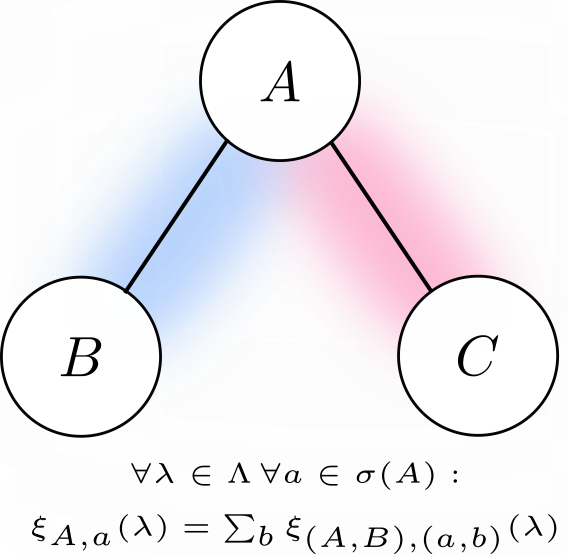
\includegraphics[width=0.4\textwidth]{images/trianglegraph.png}
    \caption{Summary of the notion of KS non-contextuality in terms of Hermitian operators. $A,B$ and $B,C$ are assumed to be commuting operators, whereas $B$ and $C$ do not commute. For every ontic state $\lambda\in\Lambda$, a deterministic non-contextual HVM assigns simultaneous eigenvalues $(a,b)$ to the commuting operators ${A,B}$. Context independence requires that taking the marginal of the joint statistics $\xi_{(A,B),(a,b)}$ must reduce to the single operator assignment $\xi_{A,a}$.}
    \label{fig:trianglegraph}
\end{figure}

An important consequence of Condition 2 in Definition \ref{def:kscontherm} is often coined “functional consistency” \cite{Peres2002}. We will only need and prove the property of “functional consistency” for functional relationships which are polynomial, however it could be extended to smooth functions with a converging (multivariate) Taylor expansion. Note that, strictly speaking, context independence implies Condition 2, as permissible outcomes of joint measurements are by definition simultaneous eigenvalues.

\begin{lemma}[functional consistency]\label{lem:funcconsist}\hfill\break Let $\nu_{\lambda}:\operatorname{Herm}(\mathcal{H})\rightarrow\mathbb{\mathbb{R}}$ be a KS non-contextual value assignment, according to Definition \ref{def:kscontherm}, and let $f:\mathbb{R}^{n}\rightarrow\mathbb{R},\thinspace(x_{1},x_{2},\dots,x_{n})\mapsto f(x_{1},x_{2},\dots,x_{n})$ be a polynomial function in $n$ real variables. Further assume that $f(X_{1},X_{2},\dots,X_{n})=0$ holds as an operator identity among the observables of a pairwise commuting set $\{X_{1},X_{2},\dots,X_{n}\}\subset\operatorname{Herm}(\mathcal{H})$. Here $f(X_{1},X_{2},\dots,X_{n})$ is the operator expression obtained by formally inserting operators $X_{i}$ into the real variables $x_{i}$. Then it must hold that $f(\nu_{\lambda}(X_{1}),\nu_{\lambda}(X_{2}),\dots,\nu_{\lambda}(X_{n}))=0$. 
\end{lemma}

\begin{proof}
By definition, the value assignment $\nu_{\lambda}$ assigns simultaneous eigenvalues to the set of pairwise commuting operators. This means that there exists a joint eigenvector $\mathcal{H}\ni\left|\Psi\right\rangle \neq0$ that corresponds to the eigenvalues assigned by $\nu_{\lambda}$. The operator expression $f(X_{1},X_{2},\dots,X_{n})$ is a sum containing terms of the form $c\prod_{i=1}^{n}X_{i}^{\alpha_{i}}$, with $c\in\mathbb{R}$, $\alpha_{i}\in\mathbb{N}_{0}$. Acting with $f(X_{1},X_{2},\dots,X_{n})$ on the joint eigenvector $\ket{\Psi}$ thus “evaluates” $f$ at $(\nu_{\lambda}(X_{1}),\nu_{\lambda}(X_{2}),\dots,\nu_{\lambda}(X_{n})):$\begin{equation*}
f(X_{1},X_{2},\dots,X_{n})\ket{\Psi} =f(\nu_{\lambda}(X_{1}),\nu_{\lambda}(X_{2}),\dots,\nu_{\lambda}(X_{n}))\ket{\Psi} =0.\end{equation*} This concludes the proof, as $\ket{\Psi}$  is non-zero.
\end{proof}

\begin{corollary}
\label{cor:funcconsist}
Let $X_1$, $X_2$ be arbitrary commuting observables and $\nu_{\lambda}:\operatorname{Herm}(\mathcal{H})\rightarrow\mathbb{R}$ a KS non-contextual value assignment. It holds that:
\begin{enumerate}
\item{$\nu_{\lambda}(X_1+X_2)=\nu_{\lambda}(X_1)+\nu_{\lambda}(X_2)$ \footnote{Compare this to the much stronger assumption made by Neumann in his faulty no-go theorem, namely that this relation must hold for arbitary observables. While this produces a contradiction already in two dimensional Hilbert spaces, the unfounded assumption has been mocked as silly by Mermin \cite{Mermin1993}.}}
\item{$\nu_{\lambda}(X_1X_2)=\nu_{\lambda}(X_1)\nu(X_2)$}
\end{enumerate}
\end{corollary}

\begin{proof}\hfill
\begin{enumerate}
\item{Define $X=X_1+X_2$, which commutes with both $X_1$ and $X_2$, and apply Lemma \ref{lem:funcconsist} to the operator identity $X-X_1-X_2=0$.}
\item{$X_1X_2$ is a Hermitian operator that commutes with both $X_1$ and $X_2$. Apply Lemma \ref{lem:funcconsist} to the operator identity $(X_1X_2)-(X_1)(X_2)=0$.}
\end{enumerate}
\end{proof}
Let us now turn to the definition of KS non-contextuality in terms of rays in a projective Hilbert space.

\begin{definition}
\label{def:kscontbasis}
Let $\mathcal{H}$ be the system Hilbert space and represent measurements as in Definition \ref{def:projmntsbasis}. A deterministic HVM is \emph{KS non-contextual} if for all ontic states $\lambda\in\Lambda$ there is a value assignment $\omega_{\lambda}:\mathcal{P}(\mathcal{H})\rightarrow\{0,1\}$ satisfying:
\begin{enumerate}
    \item (context independence)\hfill\break$\forall\ket{\Psi} \in\mathcal{P}(\mathcal{H})$, $\forall$ measurements $\mathcal{M}$ with $\ket{\Psi} \in\mathcal{M}\thinspace:\thinspace \omega_{\lambda}(\ket{\Psi} )=\xi_{\mathcal{M},\ket{\Psi} }(\lambda)$
    \item (exactly one outcome)\hfill\break $\forall$ measurements $\{\ket{\Psi_{i}} \}_{i}\subset\mathcal{P}(\mathcal{H})$ it holds that $\sum_{i}\omega_{\lambda}(\ket{\Psi_{i}})=1$
\end{enumerate}
\end{definition}

The interpretation is as follows: think of a measurement $\{\ket{\Psi_{i}} \}_{i}\subset\mathcal{P}(\mathcal{H})$ as a set of yes/no questions posed to the system. For each outcome $\ket{\Psi_{k}}$, a measurement ``asks” if this is a true property of the system, fixed by its ontic state, and subsequently ``reveals” the answer:

Given the ontic state of the system, a general deterministic HVM simultaneously fixes all possible measurement outcomes via the indicator functions $\xi_{\mathcal{M},k}(\lambda)$. This gives us an assignment similar to that above, with the crucial difference that the value assigned to an outcome $\ket{\Psi_{k}}$  may a priori depend on the measurement (ONB) it is regarded to be part of. This ONB is referred to as the ``measurement context”. For our HVM to be consistent with the interpretation of measurements revealing ``true” properties of the system, an outcome being true or false should not depend on what measurement it is a part of. The assumption of KS non-contextuality imposes that the value assigned to any ray be independent of the measurement context, meaning that a ray appearing in multiple measurements must receive the same valuation by the indicator functions, allowing for a functional dependence on only the ray itself. Lastly, Condition 2 ensures that exactly one measurement outcome corresponds to a true property of the system, which is revealed upon performing the measurement. The key points of Definition \ref{def:kscontbasis} are summarized in Figure \ref{fig:onb}, which depicts two measurement bases, assuming a three dimensional Hilbert space.

\begin{figure}
    \centering
    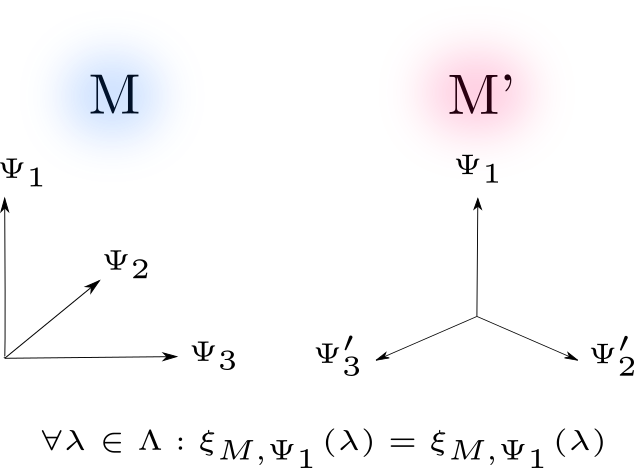
\includegraphics[width=0.5\textwidth]{images/onb.png}
    \caption{Summary of the key points of KS non-contextuality, in terms of vectors in a projective Hilbert space, depicted here to be three-dimensional. The two ONB, $\{\ket{\Psi_1}, \ket{\Psi_2}, \ket{\Psi_3}\}$ and $\{\ket{\Psi_1}, \ket{\Psi_2'}, \ket{\Psi_3'}\}$ are by a rotation in the plane. As $\ket{\Psi_1}$ appears in both measurements, a non-contextual HVM must assign the same conditional probability of observing the corresponding outcome for every ontic state $\lambda\in\Lambda$.}
    \label{fig:onb}
\end{figure}

As previously stated, both definitions of KS non-contextuality, Definitions \ref{def:kscontherm} and \ref{def:kscontbasis}, are equivalent in the following sense:

\begin{lemma}
\label{lem:equivkscont}
Let $\mathcal{H}$ be a Hilbert space. A non-contextual deterministic value assignment $\hfill\break\omega:\mathcal{P}(\mathcal{H})\rightarrow\{0,1\}$ according to Definition \ref{def:kscontbasis} induces a non-contextual deterministic value assignment $\nu:\operatorname{Herm}(\mathcal{H})\rightarrow\mathbb{\mathbb{R}}$ according to Definition \ref{def:kscontherm}, and vice versa.
\end{lemma}

Lemma \ref{lem:equivkscont} implies that proving the impossibility of a non-contextual deterministic value assignment $\omega:\mathcal{P}(\mathcal{H})\rightarrow\{0,1\}$ for Hilbert spaces of dimension $\geq3$, which we will demonstrate in the next section, entails the impossibility of a non-contextual deterministic HVM according to either definition, as such a HVM would come with a mapping $\nu$ and $\omega$ for every ontic state $\lambda$.

\begin{proof}\emph{(of Lemma \ref{lem:equivkscont})} We prove both implications separately.\begin{itemize}
\item $\nu\Rightarrow\omega$\thinspace: Define $\omega(\left|\Psi\right\rangle )\coloneqq\nu(\left|\Psi\right\rangle \left\langle \Psi\right|)$. Projectors $\left|\Psi\right\rangle \left\langle \Psi\right|$ have eigenvalues {0,1}, therefore $\omega$ maps to $\{0,1\}$. Since orthogonal projectors commute, by the property of ``functional consistency", in particular Corollary \ref{cor:funcconsist}, we get:
\begin{equation*}
    \{\left|\Psi_{i}\right\rangle \}_{i}\subset\mathcal{H} \text{ an ONB } \Rightarrow\sum_{i}\omega(\left|\Psi_{i}\right\rangle )=\sum_{i}\nu(\left|\Psi_{i}\right\rangle \left\langle \Psi_{i}\right|)=\nu(\sum_{i}\left|\Psi_{i}\right\rangle \left\langle \Psi_{i}\right|)=\nu(\mathbb{1}_{\mathcal{H}})=1.\end{equation*}

\item $\omega\Rightarrow\nu$: (Adapted from \cite{Pusey2019}) Define $\nu(A=\sum_{i,j}a_{i}|\Psi_{j}^{(i)}\rangle\langle\Psi_{j}^{(i)}|)\coloneqq\sum_{i,j}a_{i}\thinspace\omega(|\Psi_{j}^{(i)}\rangle)$, where we have used that every Hermitian operator can be spectrally decomposed. We take the eigenvalues $a_{i}$ to be distinct, $\{|\Psi_{j}^{(i)}\rangle\}_{j}$ being an ONB of the eigenspace corresponding to the eigenvalue $a_{i}$. The spectral decomposition of a Hermitian operator is not unique, as we may choose different ONB of the eigenspaces, nonetheless the above assignment is well-defined: Take
\begin{equation*}
    A=\sum_{i,j}a_{i}|\Psi_{j}^{(i)}\rangle\langle\Psi_{j}^{(i)}|=\sum_{i,j}a_{i}|\Phi_{j}^{(i)}\rangle\langle\Phi_{j}^{(i)}|
\end{equation*}
to be two spectral decompositions of $A$. Both $\{|\Psi_{j}^{(i)}\rangle\}_{j}$ and $\{|\Phi_{j}^{(i)}\rangle\}_{j}$ span the eigenspace corresponding to the eigenvalue $a_{i}$. We can extend both subsets to ONB of $\mathcal{H}$ by adding an orthonormal set $\{|\Theta_{k}\rangle\}_{k}$ to each. By the defining property of $\omega$ we get
\begin{equation*}
    \sum_{j}\omega(|\Psi_{j}^{(i)}\rangle)=\sum_{j}\omega(|\Phi_{j}^{(i)}\rangle)
\end{equation*} 
for all i, which means that $\nu$ is well-defined. Suppose $\{A,B,...\}\subset\operatorname{Herm}(\mathcal{H})$ is a set of mutually commuting Hermitian operators. There exists a shared ONB of eigenvectors $\{\left|\Psi_{i}\right\rangle \}_{i}$. Let 
\begin{align*}
    A & =\sum_{i}a_{i}\left|\Psi_{i}\right\rangle \left\langle \Psi_{i}\right| \text{ and } B =\sum_{i}b_{i}\left|\Psi_{i}\right\rangle \left\langle \Psi_{i}\right|
\end{align*}
be spectral decompositions of $A$ and $B$, where the eigenvalues $a_{i}$, $b_{i}$ can now be repeating. The assignment $\nu$ maps $A$ and $B$ to
\begin{align*}
    \nu(A) =\sum_{i}a_{i}\omega(\left|\Psi_{i}\right\rangle ) \text{ and } \nu(B)  =\sum_{i}b_{i}\omega(\left|\Psi_{i}\right\rangle ).
\end{align*}
Thus, commuting operators are mapped to simultaneous eigenvalues, and $\nu$ is a KS non-contextual value assignment like in Definition \ref{def:kscontherm}.
\end{itemize}
\end{proof}

\section{Formal statement and proof of the KS Theorem}
\label{sec:formalproof}

The KS Theorem was first proved by Kochen and Specker in 1968 \cite{Kochen1968}. Previously, Bell independently proved that a deterministic HVM of QM that induces a non-contextual value assignment like in Definition \ref{def:kscontbasis}, must be contextual \cite{Bell1966}. However his proof was deemed less convincing, as it used a continuum of vector directions, as opposed to an explicit finite set \cite{Mermin1993}.

We are now ready to reformulate the KS Theorem in precise mathematical terms (adapted from \cite{Pusey2019}):

\begin{theorem}[Kochen-Specker \cite{Kochen1968}]\hfill\break
\label{thm:ksthm}
For all projective Hilbert spaces $\mathcal{P}(\mathcal{H})$ of dimension $\geq3$, there exists a finite set $S\subset\mathcal{P}(\mathcal{H})$ of rays for which no valid value assignment $\omega:S\rightarrow\{0,1\}$ exists, satisfying the conditions for a KS non-contextual model, according to Definition \ref{def:kscontbasis}.
\end{theorem}

The existence of such a set $\mathcal{S}$ is in contradiction with any attempt of a KS non-contextual deterministic HVM of QM, as KS non-contextuality implies a valid value assignment for every possible ontic state of the system. Thus the KS Theorem effectively states the impossibility of a non-contextual deterministic HVM. 

As Pusey notes \cite{Pusey2019}, all assumptions (outcome determinism, context independence and Hilbert spaces of dimension $\ge3$) of the KS Theorem are necessary for the proof of impossibility. If we allow for context dependence, such a value assignment can be given for all sets $\mathcal{S}$, as we can assign appropriate values for each measurement contained in $\mathcal{S}$. Furthermore, relaxing the assumption of outcome determinism to an assignment of probabilities $\tilde{\omega}:\mathcal{S}\rightarrow\left[0,1\right]$ spoils the proof of impossibility, as a valid value assignment $\tilde{\omega}$ is given for instance by the Born rule: $\tilde{\omega}(\ket{\Psi_{i}} )\coloneqq\operatorname{tr}(\rho\ket{\Psi_{i}} \bra{\Psi_{i}})$ for some non-negative (Hermitian) operator $\rho$ with $\operatorname{tr}(\rho)=1$. Lastly, for Hilbert spaces of dimension 2, it is possible to give an explicit form of a non-contextual deterministic HVM \cite{Mermin1993}. The deeper reason for why our proof does not extend to the two-dimensional case is that it makes heavy use of overlapping ONB (measurement contexts) in the construction of $\mathcal{S}$, meaning different measurements that share at least one ray. These will be key in establishing a contradiction for dimensions $\geq3$. However, for two-dimensional Hilbert spaces, it is impossible to construct overlapping and distinct ONB, as a single ray fixes the ONB.

The proof of the KS Theorem is by induction with respect to to the dimension. The following Lemma (induction step), once proven, reduces the proof of the KS Theorem to the three-dimensional base case. We will prove the three-dimensional base case by giving an explicit set of directions belonging to overlapping orthogonal triads, for which a KS non-contextual value assignment can be shown to be impossible. This will be demonstrated by a chain of geometric arguments.

\begin{lemma}[\cite{Pusey2019}]\hfill\break
Assume that all projective Hilbert spaces of dimension d have a finite subset like in the KS Theorem. Let $\mathcal{P}(\mathcal{H})$ be a projective Hilbert space of dimension d+1. Then $\exists\thinspace\mathbb{\mathcal{S}\in\mathcal{P}}(\mathcal{H})$ with the same properties. 
\end{lemma}

\begin{proof}
We follow \cite{Pusey2019}. Let $\{\ket{0},\dots,\ket{d} \}$ be an ONB of $\mathcal{H}$ and let $\mathcal{H}_{0}$, $\mathcal{H}_{1}\subset\mathcal{H}$ be the d-dimensional subspaces orthogonal to $\ket{0}$, $\ket{1}$, respectively. There exist subets $\mathcal{S}_{0}$, $\mathcal{S}_{1}$ of $\mathcal{P}(\mathcal{H}_{0})$, $\mathcal{P}(\mathcal{H}_{1})$, for which there are no valid value assignments within the respective projective Hilbert space. Let $\mathcal{S}_{0}'$, $\mathcal{S}_{1}'$ denote the embeddings of $\mathcal{S}_{0}$, $\mathcal{S}_{1}$ into $\mathcal{H}$. We will show that $\mathcal{S}'\coloneqq\mathcal{S}_{0}'\cup\mathcal{S}_{1}'\cup\{\ket{0},\dots, \ket{d}\}$ then defines a subset of $\mathcal{P}(\mathcal{H})$ for which there is no valid value assignment. As $\{\ket{0},\dots,\ket{d} \}$ constitutes an ONB, a valid value assignment $\omega'$ has to map $\ket{0}$ or $\ket{1}$  (or both) to 0. Both $\omega'(\ket{0})=0$ and $\omega'(\ket{1})=0$ lead to a contradiction: For instance, say $\omega'(\ket{0})=0$. For any ONB $M\subset\mathcal{H}_{0}$ and its embedding $M'\subset\mathcal{H}$ we have
\begin{equation*}
\sum\limits _{\ket{\Psi_{i}}\in M'}\omega'(\left|\Psi_{i}\right\rangle )+\omega'(\ket{0} )=\sum\limits _{\ket{\Psi_{i}}\in M'}\omega'(\ket{\Psi_{i}})=1.     
\end{equation*}
Hence, $\omega:\mathcal{S}_{0}\mapsto\{0,1\}$, $\omega(\ket{\Psi} )\coloneqq\omega'(\ket{\Psi'})$ defines a valid value assignment, where $\ket{\Psi'} \in\mathcal{S}_{0}'$ is the embedding of $\ket{\Psi} \in\mathcal{S}_{0}$ into $\mathcal{H}$. This is a contradiction, as such an assignment does not exist for $\mathcal{S}_{0}$.
\end{proof}
What remains is a proof for the existence of a finite dimensional subset $\mathcal{S}$ that does not permit a valid KS non-contextual value assignment for the case of three dimensions. The following lemma allows us to consider only the three-dimensional complex projective space $\mathcal{P}(\mathbb{C}^{3})$ w.l.o.g.:

\begin{lemma}
Let $\mathcal{H}_{n}$ be a n-dimensional dimensional complex Hilbert space. A valid KS non-contextual value assignment $\omega:\mathcal{P}(\mathcal{H}_{n})\rightarrow\{0,1\}$ according to Definition \ref{def:kscontbasis} induces a valid value assignment $\tilde{\omega}:\mathcal{P}(\mathbb{C}^{n})\rightarrow\{0,1\}$.
\end{lemma}

\begin{proof}
Let $\{\left|\Psi_{i}\right\rangle \}_{i\in\{1,\dots,n\}}$ be an ONB of $\mathcal{H}_{n}$. We can construct the isomorphism $\mathcal{J}:\mathcal{\mathcal{H}}_{n}\rightarrow\mathbb{C}^{n}$, $\ket{\Psi_{k}} \mapsto e_{k}$ , where $\{e_{i}\}_{i\in\{1,\dots,n\}}$ is the standard basis of $\mathbb{C}^{n}$. This isomorphism preserves the inner product structure, as it maps an ONB of $\mathcal{H}_{n}$ to an ONB of $\mathbb{C}^{n}$. Thus, $\mathcal{J}$ preserves all orthogonality relations. A valid non-contextual value assignment according to Definition \ref{def:kscontbasis} then induces a valid non-contextual value assignment $\tilde{\omega}:\mathcal{P}(\mathbb{C}^{n})\rightarrow\{0,1\}$ via $\tilde{\omega}\coloneqq\omega\circ\mathcal{J}^{-1}$.
\end{proof}

Having reduced the proof of the three-dimensional base case to proving the impossibility of a valid non-contextual value assignment $\tilde{\omega}:\mathcal{P}(\mathbb{C}^{3})\rightarrow\{0,1\}$, we will now turn our attention to this task. Lemma \label{lem:3dbasecase} sticks to Peres' notation \cite{Peres1991} for saving space:

\begin{lemma}
\ref{lem:3dbasecase}
Let $\bar{1}$ denote -1 and 2 denote $\sqrt{2}$. For the following set of 33 vectors $\mathcal{S}\subset\mathbb{R}^{3}\subset\mathbb{C}^{3}$ (“Peres configuration” \footnote{For a nice visualization of the “Peres configuration”, see Conway and Kochen's paper “The Strong Free Will Theorem”, which also makes use of it \cite{Conway2011}.} \cite{Peres1991}) it is impossible to assign values $\{0,1\}$ to each vector such that for all orthogonal triads contained in $\mathcal{S}$ exactly one member receives the valuation 1:
\begin{equation*}
\begin{split}
\mathcal{S}= \{ & 100,010,001,110,101,011,1\bar{1}0,\bar{1}01,0\bar{1}1,1\bar{1}2,\bar{1}12, \\
& \bar{2}01,021,102,\bar{2}11,211,\bar{1}02,201,\bar{1}\bar{1}2,112,0\bar{2}1,012, \\
& 1\bar{2}1,121,0\bar{1}2,12\bar{1},\bar{1}21,21\bar{1},2\bar{1}1,\bar{2}10,1\bar{2}0,120,210\} 
\end{split}
\end{equation*}
Here, the tuple $\bar{2}01$ for instance corresponds to the vector 
$\begin{pmatrix}
\text{-}\sqrt{2}\\
0\\
1
\end{pmatrix}\in\mathbb{R}^{3}.$
\end{lemma}

We consider unnormalized vectors only for convenience as this does not affect orthogonality relations. 

The cubic symmetry of the set $\mathcal{S}$ greatly simplifies the proof. More precisely, the set $\mathcal{S}$ is invariant under interchange of the $x,y,z$ axes and under a reversal of the direction of each axis $x\mapsto\bar{x}$. It is the case that \begin{equation*}
\omega:\mathbb{\mathcal{S}\rightarrow}\{0,1\}\text{ a valid value assignment}\iff\omega\circ T\text{ a valid value assignment,}\end{equation*}
$T$ being one of the aforementioned symmetry transformations. This is straightforward to see, as the symmetry transformations of $\mathcal{S}$ are orthogonal transformations that leave orthogonality relations unchanged. The following concrete example shows how we can exploit the symmetry of $\mathcal{S}$ to make arbitrary assignments w.l.o.g.: Consider the orthogonal triad $\{001,100,010\}$. Assuming there exists a valid value assignment $\omega:\mathbb{\mathcal{S}\rightarrow}\{0,1\}$, then exactly one of the three vectors in the triad is assigned a 1. Due to the symmetry of the set $\mathcal{
S}$, there must be a valid value assignment $\omega'$ that assigns 001 the value 1. Analogous considerations apply to symmetry transformations $x\mapsto\bar{x}$. 

On a historical note, the original KS paper \cite{Kochen1968} gives an explicit set of 117 directions in $\mathbb{R}^{3}$ that lead to a contradiction. The current record holders are Kochen and Conway, with a set of 31 directions, however their set is not as highly symmetric as the Peres configuration, which complicates the proof \cite{Peres2002}.

\begin{proof} \emph{(of Lemma \ref{lem:3dbasecase})}\hfil\break
The proof of Lemma \ref{lem:3dbasecase} is given by the table in Figure \ref{fig:ksproof} and shows that any attempt to construct a valid KS non-contextual value assignment $\omega:\mathbb{\mathcal{S}\rightarrow}\{0,1\}$ inevitably leads to a contradiction. Finding such an assignment is equivalent to a colouring problem. Identifying 0 $\equiv$ ``green'', 1 $\equiv$ ``red'', a valid value assignment corresponds to a colouring of the rays in $\mathcal{S}$, in accordance with with the rule that each orthogonal triad in $\mathcal{S}$ must have exactly one element coloured red and two elements coloured green. Such a colouring of rays is shown to be impossible, making use of the fact that $\mathcal{S}$ contains rays that are part of multiple distinct orthogonal triads. Each line of the table introduces a new orthogonal triad that is coloured, either w.l.o.g.\ , making use of the symmetry of $\mathcal{S}$, or according to the values of previous triads. In each line, only the first ray of the triad is coloured green. The “Other rays” in each line are orthogonal to the single green ray in that line and are consequently coloured red. The stepwise colouring of rays leaves the set $\{100,021,0\text{\ensuremath{\bar{1}}2}\}$ coloured red. As these rays form an orthogonal triad, this proves that a valid colouring and thus a valid value assignment are impossible.
\end{proof}

\begin{figure}
\centering
\begin{subfigure}{\textwidth}
\centering
 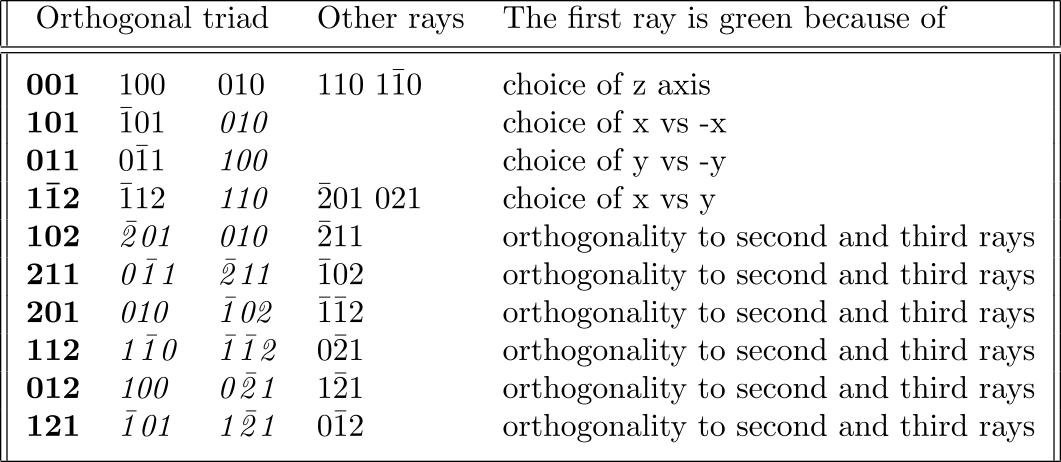
\includegraphics[width=\textwidth]{images/perestable.png}
 \caption{Table containing the proof of the three-dimensional base case of the KS Theorem, in terms of a colouring problem where each orthogonal triad must contain exactly one green and two red rays. Each line of the table introduces a new orthogonal triad that is coloured, either w.l.o.g.\ or according to the values of previous triads. In each line, only the first ray of the triad is coloured green. The ``Other rays'' in each line are orthogonal to the single green ray in that line and are consequently coloured red. The stepwise colouring of rays leaves the orthogonal triad \{100,021,0\text{$\bar{1}$2}\} coloured red, proving the impossiblity of a valid colouring. Table copied from \cite{Peres1991}.}
 \label{fig:table}
\end{subfigure}
\hfill\break
\begin{subfigure}{\textwidth}
\centering
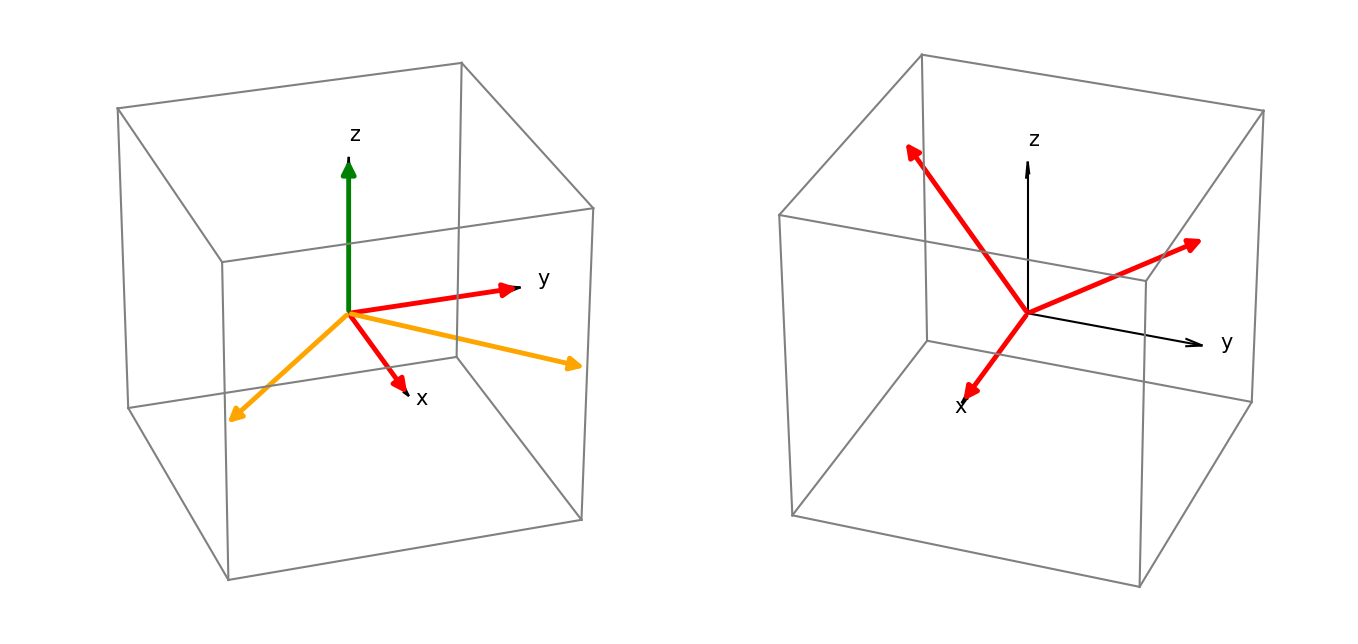
\includegraphics[width=\textwidth]{images/triads.png}
\caption{The left plot visualizes the first line of the proof-containing table, ``Other rays'' being coloured orange. The right plot visualizes the resulting contradiction, refer to the text.}
\label{fig:triads}
\end{subfigure}
\caption{Proof of the KS Theorem}
\label{fig:ksproof}
\end{figure}

\section{Algebraic proof in four dimensions}
\label{sec:4dim}
We now reap the fruits of our previous efforts that proved the equivalence of KS non-contextual value assignments to rays and such assignments to Hermitian operators. This allows us to give a far simpler and purely algebraic proof of the KS Theorem in four dimensions, which uses KS non-contextuality in terms of Hermitian operators. For the same reasons as in three dimensions, we can w.l.o.g.\ assume $\mathcal{H=\mathbb{C}}^{4}\cong\mathbb{C}^{2}\otimes\mathbb{C}^{2}$ \footnote{This is not to say that we are now considering two remote systems, but only provides a convenient way to define the set of operators used in the proof.}. Consider the set of operators depicted in Figure \ref{fig:4dim}. They form the so-called “Mermin Square” \cite{Mermin1993} and can be written in terms of Pauli operators. The operators are arranged such that the operators in each of the three rows, columns are mutually commuting. Additionally, the product of the three observables in the rightmost column is $-\mathbb{1}_{\mathbb{C}^{2}\otimes\mathbb{C}^{2}}$. The product of the three observables in all other columns and all rows is $+\mathbb{1}_{\mathbb{C}^{2}\otimes\mathbb{C}^{2}}$. By Corollary \ref{cor:funcconsist}, a KS non-contextual value assignment assigns values to the operators such that the product of values within one row, column is $\pm1$, in accordance with the corresponding operator identities. It follows that, by the row identities, the product of all nine values is $+1$, whereas the column identities result in a value of $-1$, a contradiction.

\begin{figure}
    \centering
    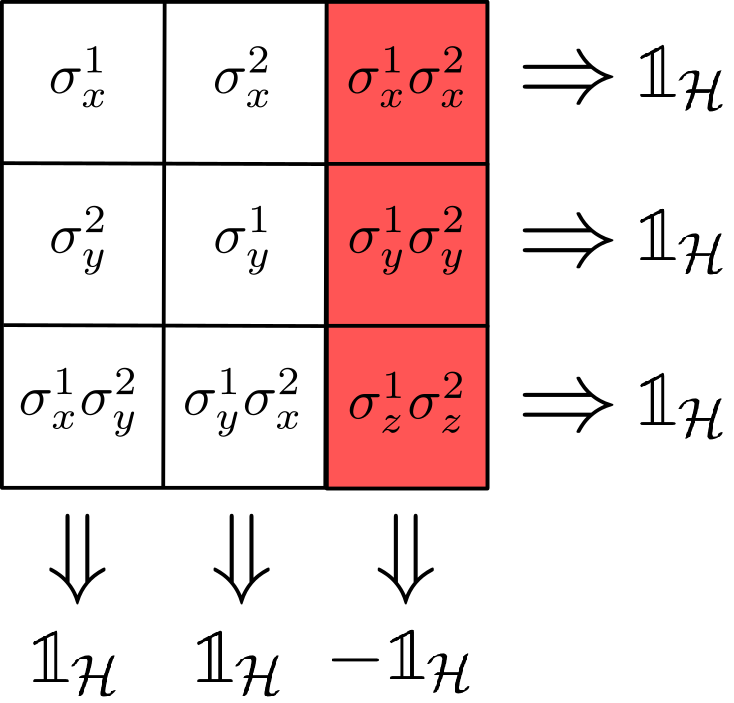
\includegraphics[width=0.6\textwidth]{images/4dim.png}
    \caption{``Mermin Square'': Operators on $\mathbb{C}^{2}\otimes\mathbb{C}^{2}$ that allow for a proof of the KS Theorem in four dimensions. Tensor products between Pauli operators are omitted for readability. Within each row and each column, the operators commute. A non-contextual value assignment to these operators is contradictory, in the sense that the product of all nine values assigned to the operators would not be well-defined. For each row, the product of the three operators in that rows is $\mathbb{1}_\mathcal{H}$. The same holds for the columns, with the notable exception that the product of the three operators in the rightmost column is $-\mathbb{1}_\mathcal{H}$. These identities on an operator level are key in establishing a contradiction. Figure adapted from \cite{Mermin1993}.}
    \label{fig:4dim}
\end{figure}

\section[Local causality and Bell's Theorem\\ Locality as an instance of KS]{Local causality and Bell's Theorem\\ \large{Locality as an instance of contextuality}}

\label{sec:bell}
The following is meant to discuss the relationship between the KS Theorem and Bell's Theorem, in particular the connection between KS non-contextuality and Bell's notion of local causality. 

Consider the well-known CHSH (thought-)experiment \cite{Clauser1969,Colbeck2019,Spekkens2012} that proves QM to be incompatible with a local HVM description. In particular, quantum theory predicts violations of the CHSH Bell inequality, which must be satisfied for all local HVM.

A source S emits pairs of entangled particles in the state $\left|\Psi\right\rangle =\frac{1}{\sqrt{2}}(\ket{\uparrow\uparrow} +\ket{\downarrow\downarrow})$ (EPR pairs) that split up and travel to two remote labs. In each of the labs, an experimenter can choose between two incompatible two-outcome measurements $A_{1}$, $A_{2}$ and $B_{1}$, $B_{2}$, respectively. One can for instance think of these as measuring different spin components of the particle. We will label the outcomes with $\pm1$. The setting of the CHSH experiment is shown in Figure \ref{fig:bell}. Let $X$, $Y$ be random variables that describe the measurement outcomes of $A_i$, $B_i$, respectively. For uniformly chosen detector settings, we wish to measure the probability
\begin{equation*}
\begin{split}
p(\text{{success}}) =\thinspace & p(X=Y,A_1,B_1)+p(X=Y,A_2,B_1) \\
& p(X=Y,A_2,B_2)+p(X\neq Y,A_1,B_2),
\end{split}
\end{equation*}
as is illustrated in Figure \ref{fig:chsh}.
All correlations compatible with a general HVM description must be of the form
\begin{equation*}
p(X=x,Y=y,A_i,B_j)=\int_{\Lambda}d\lambda\thinspace\mu(\lambda)p(X=x,Y=y\vert A_i,B_j,\lambda)p(A_i,B_j\vert \lambda),
\end{equation*}
where $\mu$ is some probability density function on the ontic state space $\lambda$.
Driven by special relativity, we further assume local causality to be a property of all valid classical descriptions: Rewriting $p(X=x,Y=y \vert A_i,B_j,\lambda)$ as $p(X=x\vert A_i, B_j, Y=y, \lambda)p(Y=y\vert A_i,B_j,\lambda)$, local causality is the assumption that, given a complete specification of the ontic state $\lambda$, the outcome of a measurement is independent of what other measurements are performed in a space-like separated region of space-time, as well as their outcomes:
\begin{align*}
    p(X=x\vert A_i,B_j,Y,\lambda) & =p(X=x\vert A_i,\lambda) \\
    p(Y=y\vert A_i,B_j,\lambda) & =p(Y=y\vert B_j,\lambda)
\end{align*}
For any ontological model of reality, local causality provides the best and most natural explanation for the fact that such superluminal influences have never been observed in experiments. Analogously, KS non-contextuality provides the most natural explanation for why, within the framework of QM, compatible observables do not disturb each other's outcome statistics. We will revisit this point in Section \ref{sec:spekkcont}, where we introduce a revised notion of contextuality due to Spekkens.
All correlations compatible with a local HVM description, i.e.\ an ontological model obeying local causality, must be of the form
\begin{equation*}
p(X=x,Y=y\vert A_i,B_j)=\int_{\Lambda}d\lambda\thinspace\mu(\lambda)p_{A}(X=x\vert A_i, \lambda)p_{B}(Y=y\vert B_j, \lambda).
\end{equation*}
The assumption of local causality for the space-like separated regions A and B manifests itself in the local response functions $p_A$ and $p_B$. W.l.o.g.\ , we can assume $p_A$ and $p_B$ to be deterministic response functions, as we may shift all classical randomness into the ontic states and the distribution $\mu$ over these. This is sometimes referred to as Fine's Theorem \cite{Fine1982}. Importantly, Fine's Theorem does not hold for general contextuality scenarios without space-like separated subsystems, as for two compatible local operators $A$, $A'$, the set of simultaneous eigenvalues is in general not given by the Cartesian product $\sigma(A)\times\sigma(A')$. We will discuss the complications that arise without space-like separated subsystems in Section \ref{sec:complicationscont}.

Assuming that the experimenters can choose the detector settings freely (no super-determinism), the choice of measurement should not be correlated with the ontic state $\lambda$ emitted by the source. Therefore, $p(A_i,B_j\vert \lambda)=p(A_i,B_j)$. All in all, for the CHSH experiment\footnote{This can of course be extended to more general correlation experiments in a Bell-like setting.} to have a valid classical \textbf{HVM description} obeying \textbf{local causality} and the assumption of \textbf{freely random detector settings}, chosen according to a \textbf{uniform distribution}, all correlations must be of the form:
\begin{equation}
\label{eqn:lhvm}
p(X=x,Y=y,A_i,B_j)=\frac{1}{4}\int_{\Lambda}d\lambda\thinspace\mu(\lambda)p_{A}(X=x\vert A_i, \lambda)p_{B}(Y=y\vert B_j, \lambda),
\end{equation}
where $p_A$ and $p_B$ are deterministic probability assignments.

Given the general expression for correlations, as prescribed by a local HVM description \ref{eqn:lhvm}, it immediately follows that $p(\text{{success}})$ is upper-bounded by $\frac{3}{4}$ for any such HVM description. This can be verified in the same manner as in Section \ref{sec:threeboxes}, where we showed deterministic and non-contextual HVM descriptions to be incompatible with Specker's three boxes: Examining Figure \ref{fig:chsh}, we realize that there is no deterministic assignment of measurement outcomes $\pm 1$ to the four measurement operators, such that all ``winning" correlations are satisfied. In fact, for any such assignment, at most three of the four ``winning" correlations are satisfied. The local response functions in Equation \ref{eqn:lhvm} induce such a deterministic assignment. Therefore, for every ontic state $\lambda$, $p(\text{success})$ is upper-bounded by $\frac{3}{4}$. The ensemble average over all ontic states $\lambda\in\Lambda$ is thus upper-bounded by the same quantity.
Consequently, $p(\text{{success}})\leq\frac{3}{4}$ is a Bell inequality: the so-called \textbf{CHSH Bell-inequality} \cite{Clauser1969,Colbeck2019,Spekkens2012}:
\begin{equation}
    \label{eqn:chshineq}
    p(\text{success}) = p(X=Y,A_1,B_1)+p(X=Y,A_2,B_1)+p(X=Y,A_2,B_2)+p(X\neq Y,A_1,B_2)\leq \frac{3}{4}
\end{equation}

In QM, outcome probabilities are computed according to the Born rule. Assuming projective measurements on a pure quantum state, permissible quantum correlations for Bell-type experiments are of the form
\begin{equation*}
p(X=x,Y=y\vert A_i, B_j)=\expval{\Pi_{A_i}^x\otimes\Pi_{B_j}^y}{\Psi},
\end{equation*}
where $\ket{\Psi}\in\mathcal{H}$ is a normalized, bipartite Hilbert state vector and $\Pi_{A_i}^x$ is the projection operator corresponding to the outcome $x$ of the measurement $A_i$ on the subsystem A.

What is remarkable about the CHSH scenario is the fact that one can give explicit projective measurements $A_{1}$, $A_{2}$, $B_{1}$, $B_{2}$, as well as the maximally entangled pure state $\ket{\Psi} =\frac{1}{\sqrt{2}}(\ket{\uparrow\uparrow} +\ket{\downarrow\downarrow})$, for which quantum theory predicts $p(\text{{success}})=\cos^{2}(\frac{\pi}{8})>\frac{3}{4}$: a violation of the CHSH Bell inequality. A set of Hermitian operators with this property is 
\begin{equation}
\label{eqn:chshmnts}
\begin{split}
A_{1} & =\ket{0}\bra{0}-\ket{\pi}\bra{\pi},\\
A_{2} & =|\frac{\pi}{2}\rangle\langle\frac{\pi}{2}|-|\frac{3\pi}{2}\rangle\langle\frac{3\pi}{2}|,\\
B_{1} & =|\frac{\pi}{4}\rangle\langle\frac{\pi}{4}|-|\frac{5\pi}{4}\rangle\langle\frac{5\pi}{4}|,\\
B_{2} & =|\frac{3\pi}{4}\rangle\langle\frac{3\pi}{4}|-|\frac{7\pi}{4}\rangle\langle\frac{7\pi}{4}|,
\end{split}
\end{equation}
with $\ket{\theta} \coloneqq\cos(\frac{\theta}{2})\ket{\uparrow} +\sin(\frac{\theta}{2})\ket{\downarrow}$ \cite{Colbeck2019}. Recall that we label the two distinct measurement outcomes with the eigenvalues $\pm 1$. Each local measurement projects the state of the particle on which it acts onto one of two antipodal surface points in the xz-plane of the single qubit Bloch sphere. As the two particles are entangled, in particular maximally correlated, measuring one particle will ``steer" the state of the other particle\footnote{This does not violate the no-signalling principle, as can be seen by computing the reduced density operator of system B: it describes a maximally mixed state.}. Thus, the probability of the measurements $(A_1,B_2)$ yielding anti-correlated outcomes is given by $\frac{1}{2}\abs{\bra{0}\ket{\frac{7\pi}{4}}}^2+\frac{1}{2}\abs{\bra{\pi}\ket{\frac{3\pi}{4}}}^2=\cos^2(\frac{\pi}{8})$. In fact, for each of the four possible measurement settings, the probability of the measurement outcomes satisfying the correlations in Figure \ref{fig:chsh} is $\cos^2(\frac{\pi}{8})$. To see this, recall that we may associate with each measurement outcome a point on the Bloch sphere, and by extension with every measurement operator an axis connecting two antipodal points on the Bloch sphere, as shown in Figure \ref{fig:chshmnts}. These axes are rotated by an angle of $\frac{\pi}{4}$ (in real space) relative to one another and lie within the xz-plane. For arbitrary $A_i$ and $B_j$, the measurement operators are chosen in such a way that the overlap of the Bloch states corresponding to measurement outcomes that obey the correlations in Figure \ref{fig:chsh} is $\cos(\frac{\pi}{8})$.

\begin{figure}
\centering
\begin{subfigure}{\textwidth}
\centering
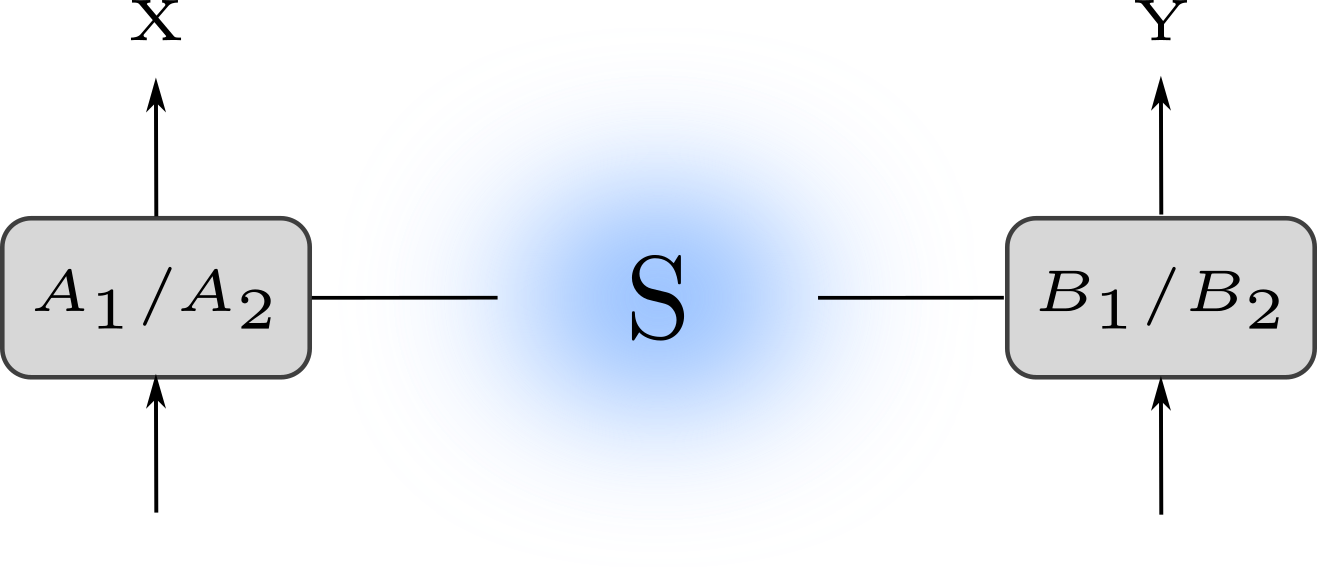
\includegraphics[width=0.8\textwidth]{images/bell.png}
\caption{CHSH setup leading to violations of the CHSH inequality. A source $S$ emits entangled EPR pairs. Constituent particles are measured in space-like separated regions, with experimenters being able to choose between two incompatible measurements $A_1$, $A_2$ or $B_1$, $B_2$. The random variables X, Y hold the measurement outcome for operators $A_1, A_2$ or $B_1, B_2$, respectively.}
\label{fig:bell}
\end{subfigure}
\vspace{2ex}
\begin{subfigure}{\textwidth}
\centering
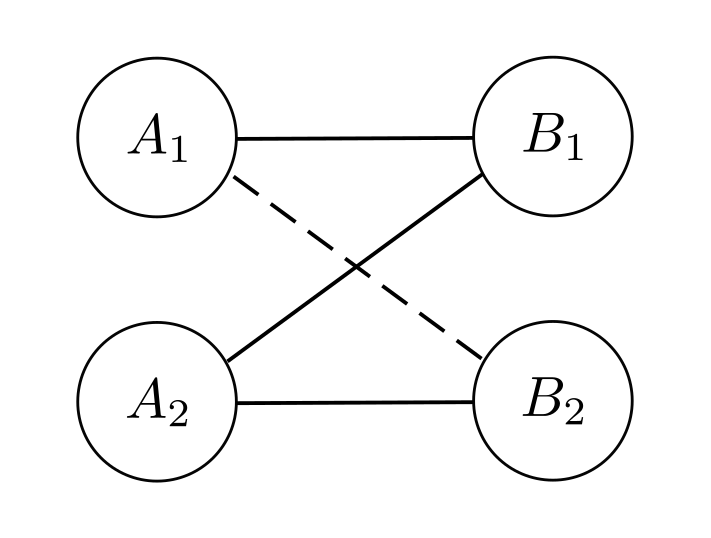
\includegraphics[width=0.6\textwidth]{images/chsh.png}
\caption{CHSH correlations for space-like separated operators $A_1$, $A_2$ and $B_1$, $B_2$. Lines indicate joint measurability. A solid line further indicates correlated outcomes, whereas a dashed line indicates anti-correlated outcomes. Let $X$, $Y$ be random variables that describe the measurement outcomes of $A_i$, $B_i$, respectively. Thus, we are interested in the probability that $X=Y$ for all choices of measurements but $(A_1,B_2)$ and $X\neq Y$ for the measurements $(A_1,B_2)$. Adapted from \cite{Spekkens2012}}
\label{fig:chsh}
\end{subfigure}
\caption{CHSH Bell test}
\label{fig:chshbelltest}
\end{figure}

\begin{figure}
    \centering
    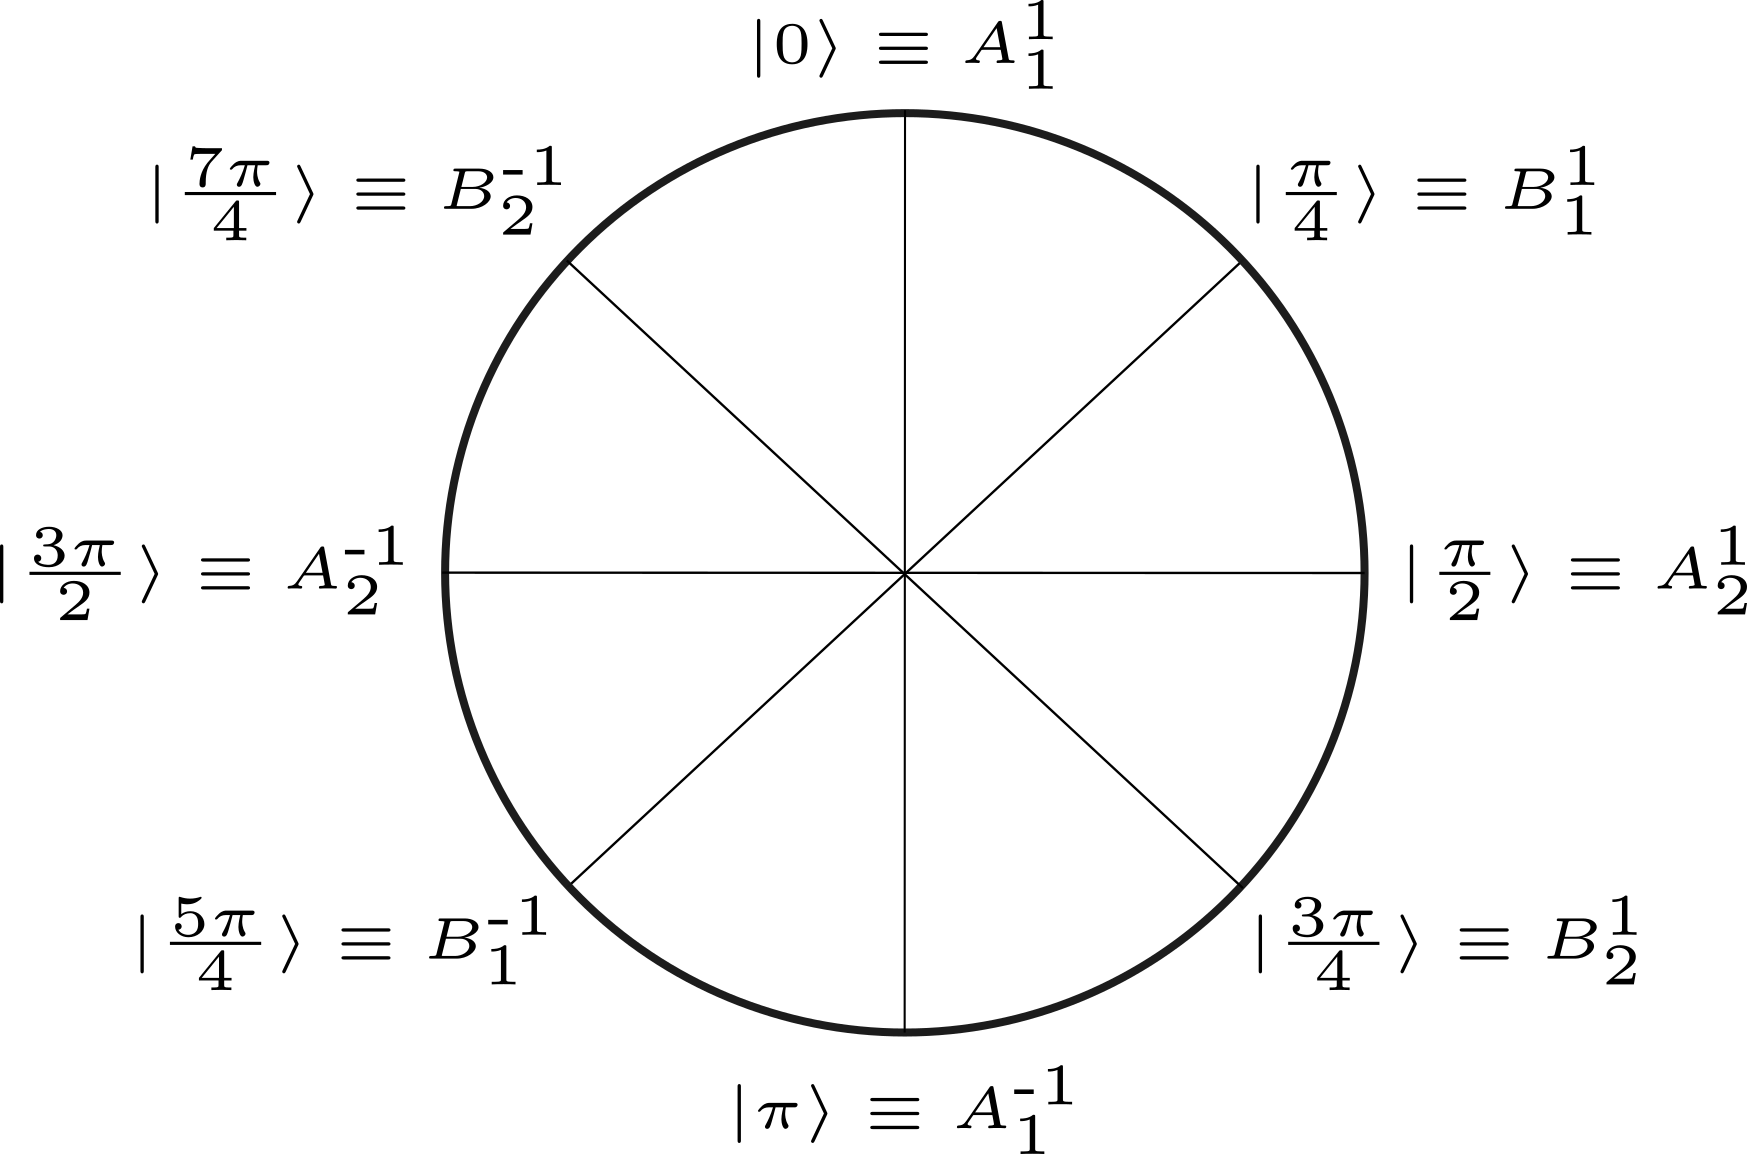
\includegraphics[width=0.7\textwidth]{images/chshmnts.png}
    \caption{The two outcomes of each of the four projective CHSH measurements $A_1$, $A_2$, $B_1$, and $B_2$ correspond to two antipodal surface points in the xz-plane of the Bloch sphere. For example, the projector associated with the outcome 1 of the measurement $A_1$ projects onto the state $\ket{0}$. The overlap between two states that are related via a rotation of $\frac{\pi}{4}$ in real space have an overlap of $\cos(\frac{\pi}{8})$.}
    \label{fig:chshmnts}
\end{figure}

In view of Section \ref{sec:self-testing}, important properties of the CHSH Bell test are:
\begin{itemize}
    \item The choice of quantum state and measurements above leads to a maximal violation of the CHSH inequality, as allowed by QM. We will show this in Section $\ref{sec:csw}$. The quantum supremum $B_\mathcal{Q}$ of a Bell inequality's left hand side is called its Tsirelson bound. The Tsirelson bound of the CHSH Bell inequality is $\frac{1}{2}(1+\frac{1}{\sqrt{2}})$.
    \item Assuming projective measurements, all quantum experiments $\expval{\Pi_{A_i}^x\otimes\Pi_{B_j}^y}{\Psi}$ producing a maximal violation of the CHSH Bell inequalitiy are essentially equivalent and related by some trivial operations. This property gives rise to the notion of self-testing and will be discussed in more detail in Section \ref{sec:self-testing}.
\end{itemize}

A generic Bell inequality in the bipartite scenario is of the form
\begin{equation}
\sum_i w_i p(\epsilon_i)\leq B_\mathcal{L}\;,
\label{eqn:bellineq}
\end{equation}
where $w_i>0$ and $\epsilon_i$ denotes the $i$-th measurement event. For now, assuming bipartite Bell tests, a measurement event can be thought of as just an initial preparation $P$ of the system (for instance in an EPR state), followed by both parties performing some local measurement $a$,$b$, and obtaining outcomes $x$,$y$: $a,b \vert x,y$. We have used the same notation as in \cite{Cabello2014} and will revisit their proposed graph-theoretic framework in more detail in Section \ref{sec:csw}, in order to identify the maximal quantum violation of a general KS non-contextuality inequality. Note that all linear combinations of probabilities pertaining to our correlation experiment can be expressed as a positive linear combination with $w_i>0$, like in \ref{eqn:bellineq}. For any negative $w_i$ we may rewrite 
\begin{equation*}
w_i p(e_i)=w_i p(x_i,y_i\vert a_i,b_i)=w_i-w_i\sum\limits_{(x_i',y_i')\neq(x_i,y_i)} p(x_i',y_i' \vert a,b)\;,
\end{equation*} obtaining a positive linear combination of probabilites. 

The statistics of a Bell-type correlation experiment are fully characterized by the set $\{p(x,y\vert a,b)\}_{x,y,a,b}$. For the CHSH experiment, this set contains $2^4=16$ values between 0 and 1, which obey some normalization conditions and can be represented by a vector in $\mathbb{R}^{16}$. Identifying permissible correlations as a subset of $[0,1]^{16}$, in the case of CHSH, one can characterize the geometry of correlations that are compatible with say local causality, quantum theory, or the no-signalling principle. Each set of permissible correlations is clearly convex: While one can check that convex combination preserves the relevant constraints, there is an intuitive argument as to why this must be the case: Assume that we have two experimental procedure, each producing ``allowed" statistics. As we only impose constraints on what correlations we consider to be ``allowed", the actual existence of such procedures cannot be discarded. We now consider the following new experimental procedure: we generate a random bit and then perform the ``old" experimental procedure corresponding to the value of the generated bit. By changing the bias of our ``coin", we can produce all statistics that are convex combinations of the initial, permissible statistics.

As discussed, all correlations $p(x,y\vert a,b)$ compatible with an ontological model obeying local causality are convex combinations of local, deterministic probability assignments $p_A(x \vert a,\lambda)p_B(y \vert b,\lambda)$. There are $2^4=16$ distinct such assignments. Thus, the set of local correlations 
\begin{equation*}
\mathcal{L} =\{\{p(x,y\vert a,b)\}_{x,y,a,b}\equiv \vec{v}\in\mathbb{R}^{16}: \vec{v}\; \text{compatible with local causality}\}
\end{equation*}
is a polytope in $\mathbb{R}^{16}$ with 16 extremal vertices. A Bell inequality \ref{eqn:bellineq} defines a separative hyperplane that splits $[0,1]^{16}$ in two, such that the closed half-space contains $\mathcal{L}$. The Bell hyperplane could for instance be a facet of the local polytope, as shown in \ref{fig:correlations}. A facet of $\mathcal{L}$ is one of its delimiting hyperplanes. Correlations that maximally violate the CHSH Bell inequality have a maximal distance to the Bell hyperplane. Bell's Theorem tells us that the set of quantum correlations $\mathcal{Q}$ is strictly larger than $\mathcal{L}$. The set $\mathcal{Q}$ cannot be characterized in terms of a finite number of delimiting hyperplanes (linear inequalities) \cite{Brunner2014}. 

The no-signalling principle is built into the tensor product representation of traditional QM. As such, the set $\mathcal{Q}$ is contained in the set $\mathcal{NS}$, which contains all correlations that obey no-signalling. Like $\mathcal{L}$, $\mathcal{NS}$ is a polytope: $\mathcal{NS}$ is the intersection of $[0,1]^{16}$, the hyperplanes corresponding to normalization constraints $\sum_{x,y} p(x,y\vert a,b)=1$, and those defined by the no-signalling conditions
\begin{align*}
\sum_y p(x,y\vert a,b) & = \sum_y p(x,y\vert a,b') \; \text{and} \\
\sum_x p(x,y\vert a,b) & = \sum_x p(x,y\vert a',b)\;.
\end{align*}
The set $\mathcal{NS}$ is strictly bigger than $\mathcal{Q}$, as there exist correlations, such as the ``PR-box", that satisfy the no-signalling principle and win the ``CHSH game" with certainty \cite{Brunner2014}.

Analogous to Bell inequalities, KS non-contextuality inequalities define hyperplanes that splits the convex set of all permissible correlations in two, such that the closed half-space contains all correlations compatible with a KS non-contextual HVM description.

\begin{figure}
    \centering
    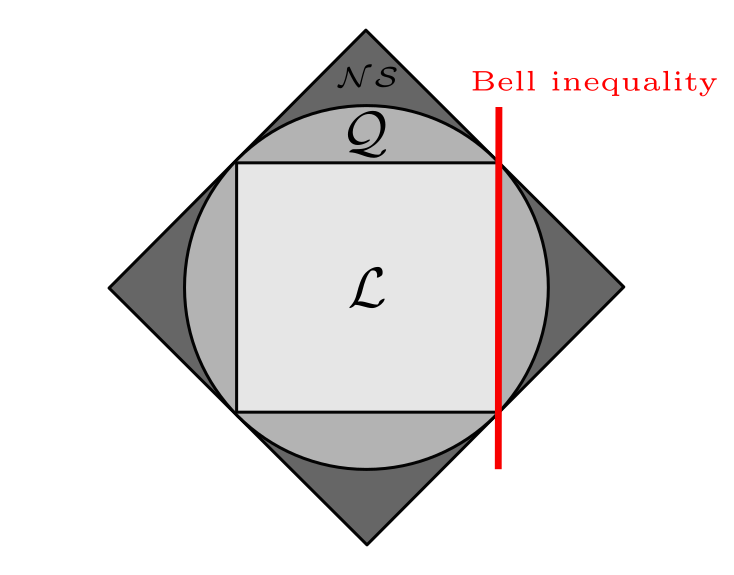
\includegraphics[width=0.7\textwidth]{images/correlations.png}
    \caption{Schematic drawing depicting the geometry of the convex sets $\mathcal{L}$, $\mathcal{Q}$, and $\mathcal{NS}$, containing all local, quantum, and no-signalling correlations, respectively. The sets $\mathcal{L}$, $\mathcal{NS}$ are polytopes and can be characterized by a finite number of facet hyperplanes, whereas the set $\mathcal{Q}$ is more complicated. A Bell inequality, like the CHSH inequality, defines a separative hyperplane such that all local correlations $\mathcal{L}$ lie to one ``side" of this hyperplane.}
    \label{fig:correlations}
\end{figure}

We have captured the essence of Bell's Theorem, cast in a quantum framework, proving that the predictions of QM are incompatible with a local HVM description. Let us now study the relationship between KS non-contextuality and Bell's notion of local causality, or equivalently local determinism (recall Fine's Theorem \cite{Fine1982}). 

The assumption of local determinism is an assumption of context independence for remote measurement contexts, like for Bell-type setting \cite{Spekkens2012}. Both boil down to measurement outcomes being independent of which remote measurement is simultaneously performed (and its outcome). It is important to keep in mind however that KS non-contextuality is a more general assumption, as compatible measurements are not required to be remote.
As Bell's Theorem implies the impossibility of a local HVM of QM, it in particular also proves the impossibility of a KS non-contextual deterministic HVM of QM. This, together with the fact that locality is accepted as a fundamental pillar of modern physics, is why Bell's Theorem is considered to be stronger than the KS Theorem. 

Informally speaking, Bell's Theorem, as presented above, is proof of a KS Theorem in four dimensions, with the nice property that KS non-contextuality is only assumed when it can be justified by locality. A caveat that stems from only assuming KS non-contextuality for remote measurement contexts is that the CHSH proof assumes an entangled state preparation $\ket{\Psi}$. In contrast, the KS Theorem, as formally stated in Theorem \ref{thm:ksthm}, is entirely measurement-dependent. Theorem \ref{thm:ksthm} states that any attempt to assign outcomes to measurements in a KS non-contextual manner is inherently contradictory, no matter the state preparation. In Section \ref{sec:4dim} we examined a KS proof in four dimensions that made use of the full extent of KS non-contextuality. Unsurprisingly, “watering down” the assumption of KS non-contextuality, like in the CHSH proof, requires us to make an additional assumption in order to arrive at a contradiction. For the CHSH proof this assumption is that of a fixed, entangled quantum state. 

Mermin gives a GHZ-like proof of an eight-dimensional KS Theorem \cite{Mermin1993}, which can be recast into a proof of Bell's Theorem, further highlighting the deep connection between both theorems. Again, the information “lost” in assuming KS non-contextuality only when justified by locality is compensated for by a fixed quantum state. Thus, the fact that the KS Theorem is only measurement-dependent and in particular makes no reference to the system preparation is a consequence of the stronger assumption of KS non-contextuality imposed by the KS Theorem.

On a final note, it is worth pointing out that the statement of the KS Theorem is of a fundamentally different nature than that of Bell's Theorem. In particular, it does not propose inequality constraints on correlations that, when found to be violated, would imply the impossibility of a particular classical description. The KS Theorem goes further than that and deduces the impossibility of such an attempt altogether, only by geometric considerations that lead to a contradiction. Nevertheless, this strength is also a key weakness of the theorem. A Bell inequality is operationally testable and does not make reference to the formalism of QM. The general form of correlations compatible with a local HVM description \ref{eqn:lhvm} makes sense, independent of QM. Therefore, the CHSH Bell inequality also holds for theories beyond QM. An experimental observation of a Bell inequality violation implies that there can be no operational theory of reality (compatible with experimental observations) that admits of a locally causal hidden variable theory, quantum theory only being one possible candidate. Any such theory would be in conflict with the experimental data which violates Bell inequalities. By comparison, the KS Theorem is formulated within the framework of QM, for instance making explicit reference to the system's Hilbert space. Therefore, the scope of the KS Theorem is limited to quantum theory. 

In Section \ref{sec:spekkcont} we revise the traditional notion of KS non-contextuality. Spekkens proposes a largely operational notion of non-contextuality that addresses these shortcomings \cite{Spekkens2005}. However, for the purposes of self-testing, which assumes the validity of QM, the main advantage of Spekkens contextuality will be that it allows for a consistent treatment of unsharp POVM quantum measurements.

\section[State-dependent KS contextuality\\ The KCBS inequality and odd n-cycle scenarios]{State-dependent KS contextuality \\ \large{The KCBS inequality and odd n-cycle scenarios}}
\label{sec:kcbs}
In Section \ref{sec:formalproof} we found that for every projective Hilbert space of dimension $\geq$ 3 there exists a finite set of rays for which there exists no KS non-contextual value assignment according to Definition \ref{def:kscontbasis}. Identifying these rays with projective measurements of rank one gives us a set of projective measurements for which there exists no KS non-contextual value assignment according to Definition \ref{def:kscontherm}. We call such sets of projective measurements (or rays in a projective Hilbert space) KS uncolourable, owing to the fact that one can reduce the problem of finding a valid KS non-contextual value assignment to a colouring problem, as was done in Section \ref{sec:formalproof}. 
\begin{definition}
A set of projective measurements (rays in a projective Hilbert space) is called \emph{KS colourable} if there exists a KS non-contextual assignment of measurement outcomes (values 0,1) to the measurements (rays) in the set. If there exists no such value assignment, the set is called \emph{KS uncolourable} 
\end{definition}
KS uncolourable sets embody the ``strongest" proofs that QM is incompatible with a KS non-contextual HVM description, in the sense that the structure in the set of measurements alone is enough to arrive at a logical contradiction.
Nevertheless, as alluded to in Section \ref{sec:bell}, also KS colourable sets of projective measurements may exhibit KS contextuality. This manifests itself in QM predicting violations of KS non-contextuality inequalities for some KS colourable sets. A KS non-contextuality inequality is, analogously to a Bell inequality, a linear inequality constraint on the convex set of correlations that is satisfied for all correlations compatible with a KS non-contextual HVM description. We will discuss the simplest KS non-contextuality inequality, the KCBS inequality, as well as an infinite class of generalizations thereof. These KS non-contextuality inequalities allow for self-testing, as will be the subject of Section \ref{sec:contselftesting}. Before that, note that we have already come across one example of a KS non-contextuality inequality, the CHSH inequality, albeit in the context of Bell nonlocality. The set of CHSH measurements given in Section \ref{sec:bell} that produce a maximal violation of the CHSH inequality when acting on an EPR pair is a KS colourable set of projective measurements. QM predicts state-dependent Bell non-locality, as witnessed by violations of the CHSH inequality. For reasons highlighted in Section \ref{sec:bell}, the CHSH inequality is also a KS non-contextuality inequality and the non-local correlations of the CHSH experiment exhibit state-dependent KS contextuality. Programming the source to emit separable bipartite states, as opposed to EPR pairs, will yield KS non-contextual correlations.

Note that there even exist KS colourable sets of measurements that produce state-independent KS contextuality, in the sense that QM predicts the violation of a KS non-contextuality inequality for all possible quantum state preparations. An example of such a set is one proposed by Yu and Oh \cite{Yu2012}, simply called the Yu-Oh set. It is a set of 13 rank one projectors that act on a three-dimensional Hilbert space. In fact, if one identifies the rank one projectors with rays in a projective Hilbert space, the 13 Yu-Oh rays are a subset of the 33 rays of the Peres configuration that we used in proving the KS Theorem in Section \ref{sec:formalproof}. The Yu-Oh set is the minimal set of rays revealing state-independent KS contextuality, as proved in \cite{Cabello2016a}.

The perhaps simplest example of a quantum experiment leading to (state-dependent) KS contextuality for a single quantum system is the KCBS scenario \cite{Klyachko2008}. We will present the corresponding KCBS KS non-contextuality inequality, which will become relevant when we later discuss self-testing of quantum systems in Sections \ref{sec:self-testing} and \ref{sec:contselftesting}. 

For the KCBS KS contextuality scenario we assume five dichotomic projective measurements with outcomes 0 and 1. Additionally, the five measurements should obey cyclic compatibility, as shown in Figure \ref{fig:kcbscompat}. We freely choose a pair of compatible measurements (measurement context) at random, each with equal probability, and determine the value of the following linear sum of probabilities:
\begin{equation*}
    \sum_{i=1}^5 p(0,1\vert i, i+1)\leq 2,
\end{equation*}
where compatibility with a KS non-contextual HVM imposes an upper bound of 2 for this expression: For any HVM description of the KCBS experiment, $\sum_{i=1}^5 p(0,1\vert i,i+1)$ can be rewritten as $\int_{\Lambda}d\lambda\thinspace\mu(\lambda\vert i,i+1)\sum_{i=1}^5 p(0,1\vert i, i+1, \lambda)$, where $\mu$ is some probability density function over the ontic state space $\Lambda$. Furthermore $\mu(\lambda\vert i,i+1)=\mu(\lambda)$ as we assume the choice of measurement context to be uncorrelated with the system. Analogously to Specker's three boxes or the CHSH experiment, one can easily verify that for a KS non-contextual HVM description this quantity has a non-trivial upper bound. 

\begin{figure}
    \centering
    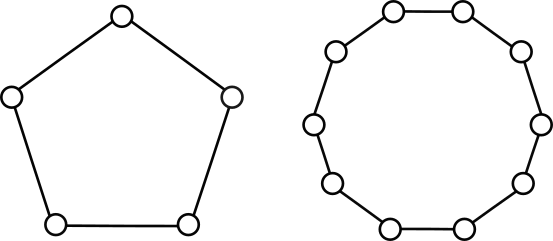
\includegraphics[width=0.7\textwidth]{images/kcbscompat.png}
    \caption{Graph showing the compatibility relations for the KCBS (left) and a higher order odd $n$-cycle scenario (right). Each vertex corresponds to one projective measurement, adjacent measurements are compatible.}
    \label{fig:kcbscompat}
\end{figure}

We now present a quantum experiment involving a KS colourable set of five projective measurements on a qutrit for which QM predicts a (maximal) violation of the KCBS KS non-contextuality inequality. The five projective measurements of this reference experiment correspond to five rank one projectors that project onto five pure qutrit states. The components of these five qutrit states with respect to the standard qutrit basis $\{\ket{0}, \ket{1}, \ket{2}\}$ are real, allowing us to represent them as vectors in $\mathbb{R}^3$, see Figure \ref{fig:kcbsref}. The angle between each of the five vectors and the $\vert 0\rangle$ qutrit axis is $\cos^2(\theta)=\frac{1}{\sqrt{5}}$. The following is an explicit expression for five suitable qutrit states that also satisfy cyclic compatibility:
\begin{align*}
    \ket{u_j} = \left(\cos(\theta),\thinspace\sin(\theta)\sin(j\phi),\thinspace\sin(\theta)\cos(j\phi)\right)^T,
\end{align*}
for $\displaystyle j=1\dots 5$ with $\displaystyle\phi=\frac{4\pi}{5}$.

For these five projective measurements acting on the $\vert 0\rangle$ qutrit state, QM predicts \begin{equation*}
\sum_{i=1}^5p(0,1\vert i, i+1)=\frac{5}{\sqrt{5}}=\sqrt{5}>2.    
\end{equation*}
Not only does the reference quantum experiment $\ket{0}$, $\{\ket{u_i}\}_{i=1}^5$ produce correlations that violate the KCBS non-contextuality inequality, but this violation is also maximal, as we will see in Section \ref{sec:csw}.

\begin{figure}
    \centering
    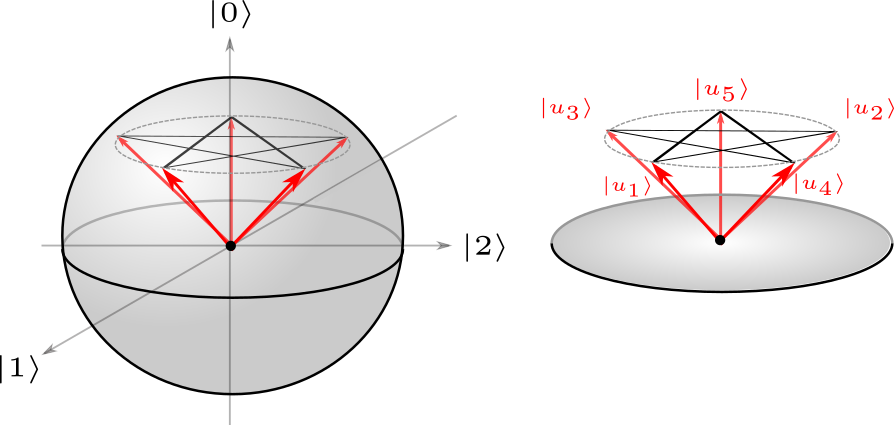
\includegraphics[width=\textwidth]{images/kcbsref.png}
    \caption{Reference KCBS experiment on a qutrit leading to a maximal violation of the KCBS KS non-contextuality inequality. An experimenter can freely choose between five rank one projective measurements $\ket{u_i}$ that satisfy cyclic compatibility: $\bra{u_i}\ket{ u_{i\oplus1}} = 0$. The qutrit is initially prepared in the state $\ket{0\rangle}$ and then measured in one of five measurement contexts (i,i$\oplus$1). After the measurement the qutrit state is ``reset".}
    \label{fig:kcbsref}
\end{figure}

One can generalize the KCBS KS non-contextuality inequality to greater cycle lengths $n$. For the odd integers $n\geq 5$, where $n$ parametrizes the number of dichotomic projective measurements obeying cyclic compatibility, one finds a class of KS non-contextuality inequalities \cite{Bharti2019}
\begin{equation}
    \label{eqn:oddncycleclass}
    \sum_{i=1}^n p(0,1\vert i,i+1) \leq \frac{n-1}{2}.
\end{equation}
The quantum supremum for a given cycle length $n$ is given by 
\begin{equation}
\label{eqn:ncyclequsup}
B_q^{(n)}=\frac{n\cos(\frac{\pi}{n})}{1+\cos(\frac{\pi}{n})}
\end{equation} and can be achieved by measuring the $\ket{0}$ qutrit state with the rank one projective measurements
\begin{equation}
\label{eqn:ncycleideal}
\vert u_j^{(n)}\rangle = \left(\cos(\theta_n),\thinspace\sin(\theta_n)\sin(j\phi_n),\thinspace\sin(\theta_n)\cos(j\phi_n)\right)^T,
\end{equation}
for $j=1\dots n$, $\displaystyle\cos^2(\theta_n)=\frac{\cos(\frac{\pi}{n})}{1+\cos(\frac{\pi}{n})}$, and $\displaystyle\phi=\frac{(n-1)}{n}\pi$.

In Section \ref{sec:csw}, we adopt the graph-theoretic framework proposed in \cite{Cabello2014} to classify correlations of an arbitrary experiment. It turns out that for a general linear combination of probabilities one can relate the KS non-contextual and quantum suprema to certain graph invariants. Computing these graph invariants corresponds to solving a mathematical optimization problem. In view of self-testing, this will enable us to identify extremal correlations and study whether these can only be realized in an essentially unique manner.
\chapter{CSW graph-theoretic approach to quantum correlations}
\lhead{\emph{CSW graph-theoretic approach to quantum correlations}}
\label{sec:csw}

In \cite{Cabello2014}, the authors propose a graph-theoretic approach to classifying the statistics of an arbitrary correlation experiment that aims to determine the value of some linear combination of probabilities. In particular, \cite{Cabello2014} identifies a hierarchical structure that classifies correlations as classical (KS non-contextual), quantum, or more generally obeying the exclusivity principle \footnote{The exclusivity applies to pairwise exclusive events and bars their added probabilities from exceeding 1. We will come back to it shortly.}. This hierarchical structure is established by associating with a correlation experiment its corresponding ``exclusivity graph". The exclusivity structure obeyed by the experiment imposes non-trivial constraints on the set of permissible correlations compatible with KS non-contextuality, QM, or the exclusivity principle. In particular, upper bounds of the relevant linear combination of probabilities, within these three classes of theories, can be related to graph invariants of the experiment's exclusivity graph.

\section{Generic correlation experiments in the CSW framework}
\label{sec:correxp}
The CSW framework takes an operationalist approach to correlation experiments, in the sense that any such experiment is described in terms of a sequence of (reproducible) experimental procedures. For example, one such experimental procedure may be to prepare the system in a certain way. If they provide the experimenter with an output (apart from the transformed system), such experimental procedures can be considered \emph{tests}. For a preparation $P$, and test $M$ with outcomes $\{k_i\}_i$, an operational theory specifies the probabilities $p(k_i\vert M,P)$. 

There may be multiple equivalent ways of preparing a system, in the sense that we can never tell the preparation procedures apart by experiment, as they yield identical probability distributions for all tests. The equivalence class of operationally indistinguishable preparation procedures $P$ defines a state. In the same manner, the equivalence class of operationally indistinguishable tests $M$ defines an observable\footnote{This identification of operationally equivalent tests and preparations parallels the operational equivalence classes we will introduce in Section \ref{sec:spekkcont}, when introducing the notion of  Spekkens contextuality.}.

We now define what it means for two observables to be compatible, or jointly measurable. While in QM two projective measurements are compatible if and only if the corresponding Hermitian operators commute, we want to define compatibility in operational terms, in order for the definition to be applicable to arbitrary operational theories.

\begin{definition}
\label{def:compat}
Two observables $M_{1}$, $M_{2}$ with outcome sets $\{k_i\}_i$ and $\{k'_i\}_{i}$, respectively, are \emph{jointly measurable} if there exists an observable $M_{12}$ with outcome set $\{k_i,k'_j\}_{i,j}$ such that:
\begin{enumerate}
\item $\forall$ preparations $P$, $\forall$ outcomes $k\in\{k_i\}_i$:\hfill\break $p(k\vert M_1,P)=\sum_{k'}p(k,k'\vert M_{12},P)$
\item $\forall$ preparations $P$, $\forall$ outcomes $k'\in\{k'_j\}_j$:\hfill\break $p(k'\vert M_2,P)=\sum_{k}p(k,k'\vert M_{12},P)$
\end{enumerate}
\end{definition}

\noindent One may think of $M_{12}$ as measuring both $M_{1}$ and $M_{2}$ simultaneously, placing the outcome of $M_{1}$ into its first and the outcome of $M_{2}$ into its second output register. By discarding one of the outcomes, we reduce $M_{12}$ to the corresponding single-outcome measurement. At the level of probability distributions, discarding one of the outcomes corresponds to a summation over all possible outcomes held by the discarded register. For QM as operational theory and projective measurements, this definition is equivalent to operator commutativity. For general quantum measurements, Definition \ref{def:compat} implies that the POVM $M_1$ and $M_2$ are obtained by coarse graining the POVM $M_{12}$ that jointly realizes both.

An \emph{event} is characterized by a list of compatible tests $(M_1, M_2, \dots, M_n)$ that yield some outcomes $(X_1, X_2, \dots, X_n)$. Let $X_1,X_2,\dots, X_n\thinspace\vert\thinspace M_1,M_2,\dots, M_n$ denote such event. Some events may be operationally equivalent, in the sense that they have the identical probability of occuring, for all initial preparations of the system. Analogous to our treatment of preparations and tests, operationally equivalent test-outcome tuples define the same event. Within QM, a state would be defined by a density operator, whereas equivalent events correspond to the same positive semi-definite operator or projector.

A correlation experiment, like the KCBS or CHSH experiment, consists of one or multiple experimenters performing subsets of compatible tests on an intial preparation $P$ of the system. For instance, in the KCBS experiment, an experimenter chooses between five measurement contexts $(i,i\oplus 1)$. We assume that an experimenter can freely choose between measurement contexts, i.e.\ subsets of compatible tests, meaning that this choice is not correlated with say the system being measured. By recording which of all could-be events occurs for many repetitions of this procedure, the experimenter(s) can determine the value of some relevant linear combination $\sum_i w_i p(\epsilon_i\vert P)$, where $w_i>0$, and $\epsilon_i$ denotes a possible event i.e.\ a set of compatible tests that yield some outcomes. Sometimes we will omit the initial preparation $P$ in our formulas. Let us now discuss what conditions and assumptions allow us to impose non-trivial constraints on correlations.

We define two events to be exclusive if they specify different outcomes for identical tests.
\begin{definition}[\cite{Amaral2018}]
\label{def:exclevents}
For outcome-repeatable tests, two events
\begin{equation*}
X_1,X_2,\dots, X_n\thinspace\vert\thinspace M_1,M_2,\dots, M_n\;\text{ and }\; X'_1,X'_2,\dots, X'_m\thinspace\vert\thinspace M'_1,M'_2,\dots, M'_m  
\end{equation*} are \emph{exclusive} if for some $i$ and $j$
\begin{equation*}
    M_i = M'_j \text{ and } X_i \neq X'_j.
\end{equation*}
\end{definition}

An important assumption that underlies the CSW framework is that all measurements are assumed to be outcome-repeatable, meaning that performing two identical tests in a consecutive manner always yields identical outcomes. As such, we can, by performing a subsequent measurement $M_i$, perfectly distinguish between two exclusive events. The assumption of outcome repeatability compells us to restrict quantum measurements to PVM, as this is not a general feature of unsharp quantum measurements. Dropping the assumption of outcome repeatability and thereby accounting for general POVM quantum measurements will not provide us with any non-trivial constraints distinguishing the set of quantum correlations from the the set of general probabilistic assignments, at least not within the CSW framework. The reason for this that the exclusivity principle, which we invoke in Section \ref{sec:cswhierarch} to obtain constraints on correlations, is in general not true for theories within which pairwise compatibility does not imply joint compatibility (Specker's ``fundamental theorem'', see Section \ref{sec:threeboxes}). There exist POVM that are pairwise compatible, but fail to satisfy joint compatibility \cite{Heunen2014}. Section \ref{sec:cswunsharp} will discuss in more detail how the CSW framework falls apart when allowing for general unsharp measurements.

For a correlation experiment with two exclusive could-be measurements events $\epsilon_1$ and $\epsilon_2$, the sum of their probabilities cannot exceed 1, for all initial preparations $P$: Take $M$ to be the test that perfectly distinguishes between $\epsilon_1$ and $\epsilon_2$, like in Definition \ref{def:exclevents}, with $\epsilon_1$ specifying the outcome $X_1$ and $\epsilon_2$ the outcome $X_2$. Imagine performing the test $M$ after one input-output round of the correlation experiment: 
\begin{align*}
1 & \geq p(\{X_1,X_2\}\vert M) \\
& \geq p(\{X_1,X_2\}\vert M, \epsilon_1)\thinspace p(\epsilon_1) + p(\{X_1,X_2\}\vert M, \epsilon_2)\thinspace p(\epsilon_2)\\
& = p(\epsilon_1)+p(\epsilon_2).
\end{align*}
The exclusivity principle extends this property to sets of pairwise exclusive events:

\begin{principle}[Exclusivity principle]\hfill\break
For a set of pairwise exclusive measurement events of a correlation experiment $\{\epsilon_i\}_i$
\begin{equation*}
    \sum_i p(\epsilon_i)\leq 1,
\end{equation*}
for all initial preparations.
\end{principle}

We denote the set of correlations that are compatible with the exclusivity principle by $E_1$.

Not all valid assignments of probabilities to events of a correlation experiment, i.e.\ probabilistic models of a correlation experiment, are compatible with the exclusivity principle. For example, consider Specker's three boxes, as introduced in Section \ref{sec:threeboxes}. The relevant linear combination of probabilities that this correlation experiment tests is
\begin{equation*}
S = \frac{1}{3}\sum_{i=1}^3\thinspace p(0,1 \thinspace\vert\thinspace i,i\oplus 1) +  \frac{1}{3}\sum_{i=1}^3\thinspace p(1,0\thinspace\vert\thinspace i\oplus 1,i).
\end{equation*}
For both sums, the events that appear are pairwise exclusive. Therefore, within theories obeying the exclusivity principle, $S$ is upper-bounded by $\frac{2}{3}$. However, by assigning the probability $\frac{1}{2}$ to each event appearing in $S$ we obtain a probability assignment that is compatible with pairwise exclusivity, but incompatible with the exclusivity principle. Furthermore, this assignment of probabilities is consistent with perfectly anti-correlated outcomes for all measurement contexts, as was considered in Section \ref{sec:threeboxes}.
While the exclusivity principle must not be true for arbitrary theories, it does apply to QM, if all measurements are projective, and by extension to KS non-contextual correlations. This can be seen by noting that exclusive events must be assigned orthogonal projectors and noting that for a set of orthogonal projectors $\{\Pi_i\}_i$, $(\thinspace\mathbb{1}-\sum_i \Pi_i\thinspace)$ is a positive semi-definite operator.
Therefore, in Section \ref{sec:cswhierarch}, we may use the exclusivity principle to impose constraints on the set of quantum (and KS non-contextual) correlations.

If we extend quantum measurements to general POVM, the exclusivity principle must no longer hold, as we just demonstrated for correlation experiments like Specker's three boxes (assign the positive operator $\frac{\mathbb{1}}{2}$ to all measurement events).

\section{The exclusivity graph of a correlation experiment}
The exclusivity graph of a correlation experiment is a convenient representation of the exclusivity structure obeyed by events that imposes constraints on what correlations are permissible within different classes of theories. 
The exclusivity graph of a correlation experiment $S=\sum_i w_i p(\epsilon_i)$ has a vertex for each measurement event $\epsilon_i$ appearing in $S$.  Furthermore, exclusive measurement events are represented as adjancent vertices, as shown in Figure \ref{fig:kcbsexclusivity} for the KCBS correlation experiment, or in Figure \ref{fig:3boxesexcl} for Specker's three boxes.


\begin{figure}
\centering
\begin{subfigure}{\textwidth}
    \centering
    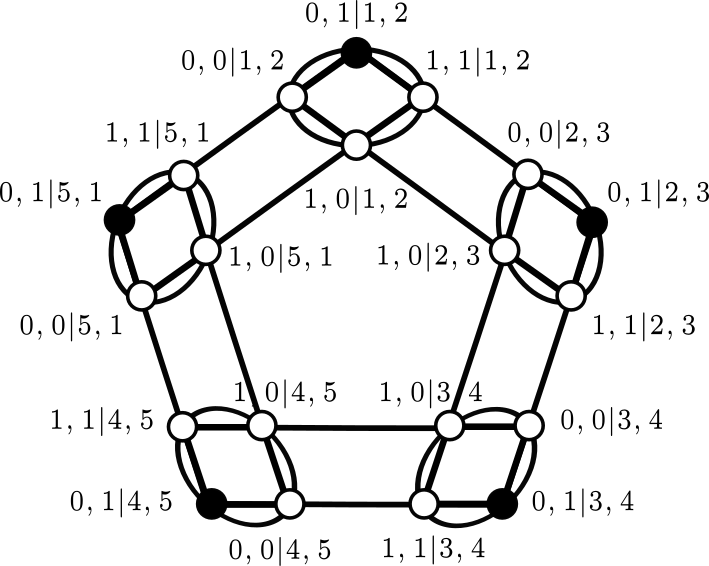
\includegraphics[width=0.6\textwidth]{images/kcbsexclusivity1.png}
    \caption{Graph depicting all events of the KCBS correlation experiment and the underlying exclusivity structure. An event is defined in terms of a measurement context and outcome tuple, and is represented by a vertex of the graph. Adjacent vertices correspond to ``mutually exclusive" events. Figure copied from \cite{Cabello2014}.}
\end{subfigure}
\break\vspace{5ex}
\begin{subfigure}{\textwidth}
    \centering 
    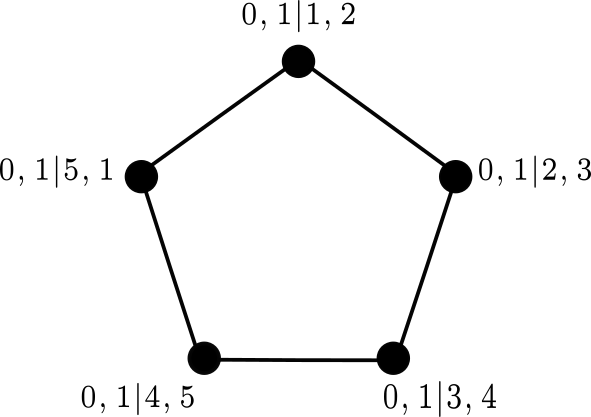
\includegraphics[width=0.6\textwidth]{images/kcbsexclusivity2.png}
    \caption{Simplified exclusivity graph for the KCBS correlation experiment. Contains only those vertices in (a) whose probabilities appear in the KCBS KS non-contextuality inequality. Figure copied from \cite{Cabello2014}.}
\end{subfigure}

\caption{KCBS exclusivity graph}
\label{fig:kcbsexclusivity}
\end{figure}


\begin{figure}
    \centering
    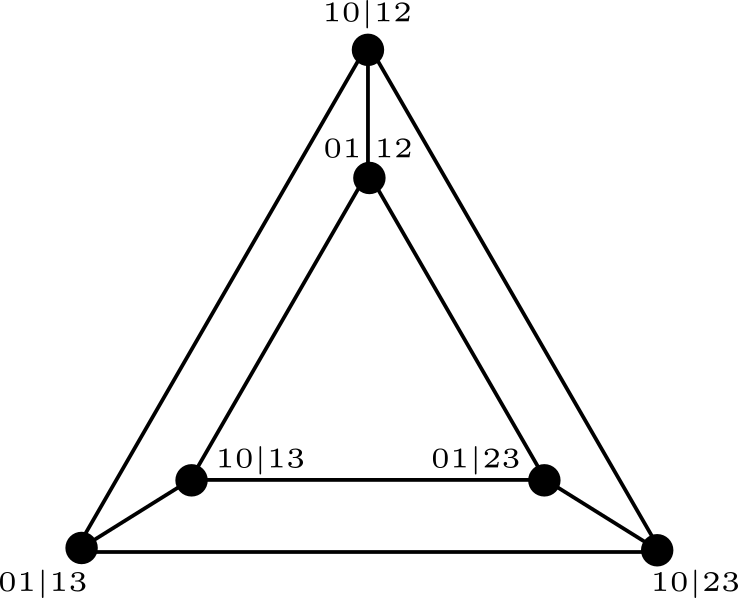
\includegraphics[width=0.5\textwidth]{images/3boxesecl.png}
    \caption{Exclusivity graph for Specker's three boxes correlations experiment, see Section \ref{sec:threeboxes}. The outcome 0 corresponds to the opened box being empty, whereas the outcome 1 corresponds to the opened box containing a gem.}
    \label{fig:3boxesexcl}
\end{figure}

\section{Hierarchical structure of correlations}
\label{sec:cswhierarch}
We will now relate upper bounds for the quantity $S$, for correlations that are compatible with KS non-contextuality, QM, or the exclusivity principle, to graph invariants of the experiment's exclusivity graph. All three graph invariants can be computed by solving a corresponding mathematical optimization problems. The proofs we present are adapted from \cite{Cabello2014}:

\begin{itemize}
    \item \textbf{KS non-contextual correlations:}
    The CSW approach decouples KS non-contextuality from the operational theory that is QM and extends it to arbitrary operational theories. For a given exclusivity graph, classical i.e.\ KS non-contextual correlations are those that can be written as a convex combination of deterministic assignments $\nu: V\mapsto\{0,1\}$ that obey the exclusivity principle, where $V$ is the vertex set of the correlation experiment. Let us verify that this extension to arbitrary operational theories is compatible with KS non-contextuality as defined in Definition \ref{def:kscontherm}: Assuming QM and projective measurements, each event defines a (distinct) projector, as we identify operationally equivalent events. Furthermore, pairwise exclusive events correspond to pairwise orthogonal projectors and can be regarded as part of the same resolution of the identity. The correlation experiment is consistent with a KS non-contextual description according to Definition \ref{def:kscontherm} if and only if all correlations are compatible with an assignment $\nu$ like above, up to convex combination. Therefore, for the case of QM as operational theory and perfectly sharp measurements, the generalized notion of classicality in \cite{Cabello2014} reduces to KS non-contextuality like in Definition \ref{def:kscontherm}.
    
    As will be discussed in Section \ref{sec:odum}, lifting the notion of KS non-contextuality as relevant criterion for non-classicality to arbitrary operational theories, and assigning outcomes in a deterministic fashion to potentially unsharp measurements, gives rise to a number of inconsistencies. Therefore, this ``incremental" \cite{Pusey2019} approach towards an operational notion of non-contextuality seems to be flawed. An alternative will be presented in Section \ref{sec:spekkensopappr}.
    
    We now wish to determine the maximal value of $S$ that is compatible with a classical description like above. For a set of pairwise adjacent vertices, the sum of the probabilities assigned to these cannot exceed 1. Only two independent vertices, meaning two vertices that are non-adjacent can both receive the valuation 1. It follows that the maximal value of $S$ is \begin{equation*}
    S_{nc}=\max\limits_{U}\;\sum_{i\in U} w_i,
    \end{equation*}
    where the expression is maximized over all independent sets of the exclusivity graph. This is the independence number of the (weighted) exclusivity graph. Section \ref{sec:kcbs} presents concrete values for the odd $n$-cycle scenarios, see Equation \ref{eqn:oddncycleclass}.
    
    \item \textbf{Quantum correlations:}
    The set of quantum correlations, restricting to projective measurements, is of the form\footnote{We can w.l.o.g.\ assume a pure quantum state. For mixed states $\ket{\rho_A}$, consider the purification $\Psi_{AE}$ and projectors $(\thinspace\Pi_i\otimes\mathbb{1}_E\thinspace)$.} \begin{equation*}
    p(\epsilon_i)=\expval{\Pi_i}{\Psi},
    \end{equation*}
    for some quantum state $\ket{\Psi}$ and $\Pi_{i}$ the projector corresponding to the event $\epsilon_i$. Adjacent events must be represented by orthogonal projectors:
    \begin{equation*}
        \Pi_{i}\Pi_{j} = 0 \text{ for } \epsilon_i, \epsilon_j \text{ adjancent}.
    \end{equation*}
    For an arbitrary quantum realization $\vert \Psi\rangle$, $\{\Pi_{i}\}_i$, define the vectors
    \[\ket{u_0} \coloneqq \ket{\Psi}\text{ and }\ket{u_i} \coloneqq \frac{\Pi_{i} \ket{u_0}}{\sqrt{\expval{\Pi_i}{u_0}}} \]
    
        
    The $(n+1)\times(n+1)$ Gram matrix\footnote{The Gram matrix $X$ of a set of vectors $v_1,\dots, v_n$ in an inner product space $(V,\langle \cdot, \cdot\rangle)$ is the $n\times n$ matrix with entries $X_{ij}=\bra{ v_i}\ket{ v_j}$. The Gram matrix of a set of vectors is positive semi-definite and all positive semi-definite matrices are the Gram matrix for some non-unique list of vectors. For a $n\times n$ positive semi-definite matrix $X$, we can always find a suitable list of vectors in $(\mathbb{C}^n, \langle \cdot, \cdot\rangle_{\text{std}})$, where $\langle \cdot, \cdot\rangle_{\text{std}}$ is the standard inner product, by computing the Cholesky decomposition of $X$. Acting with an arbitrary isometry $V:\mathbb{C}^n\rightarrow\mathbb{C}^d$, $d\geq n$, yields a Gram decomposition in $(\mathbb{C}^d,\langle \cdot, \cdot\rangle_{\text{std}})$.} $X$ of the vectors $\{\bra{u_i}\ket{u_0} \ket{u_i}\}_{i=0}^n$ obeys the following constraints:
    \begin{align*}
        X_{00} &= 1\,,\\
        X_{0i} &= X_{ii}\,,\\
        \text{and } X_{ij} &= 0 \text{ for $\epsilon_i$, $\epsilon_j$ adjacent} \\  
    \end{align*}
    Additionally, $\sum_i w_i X_{ii} = \sum_i w_i \abs{\expval{\Pi_i}{\Psi}}^2$, the value of the linear combination $S$ for the quantum model $\ket{\Psi}$, $\{\Pi_i\}_i$. As we can construct a Gram matrix that satisfies these constraints and which is related to $S$ like above for all quantum experiments , the maximum value of $S$, for a given exclusivity graph, that is compatible with QM is upper-bounded by the so-called Lovász semi-definite program (SDP) \cite{Bharti2019}
    \begin{alignat}{2}
    \label{eqn:lovaszsdp}
    \operatorname{max}\sum_{i=1}^n\; & w_i X_{ii} \nonumber\\
    \text{subject to } X_{ii} &=X_{01}\;,\hspace{1ex} && 1\leq i\leq n \\
    X_{ij} & = 0 \;, && \text{for } \epsilon_i,\; \epsilon_j \text{ adjacent} \nonumber\\
    X_{00} & = 1 \;,\; && X\in\mathcal{S}_{+}^{\thinspace n+1},\nonumber
    \end{alignat}
    where $\mathcal{S}_{+}^{1+n}$ is the set of positive semi-definite $(n+1)\times(n+1)$ matrices.
    
    One might naively think that the Lovász bound is tight: For an optimal solution of the Lovàsz SDP \ref{eqn:lovaszsdp}, $X^*$, with Gram decompostion $\{\ket{u_i}\}_{i=0}^n$, $S=\sum_{i=1}^n w_i X^*_{ii}$ can be realized by the quantum experiment which consists of an experimenter performing the rank-one projective measurements $\ket{\Tilde{u_i}} \bra{\Tilde{u_i}}$ on the state $\ket{\Tilde{u_0}}$, where the vectors $\{\ket{\Tilde{u}_i}\}_{i=0}^n$ are obtained by normalization:
    \begin{align*}
    p(\epsilon_i) =\operatorname{tr}(\ket{\Tilde{u}_i}\bra{\Tilde{u}_i} \ket{\Tilde{u}_0}\bra{\Tilde{u}_0}) = \abs{ \bra{\Tilde{u}_0} \ket{\Tilde{u}_i}} ^2 = \frac{\abs{ \bra{u_0} \ket{u_i}} ^2}{\bra{u_0}\ket{u_0}\bra{u_i}\ket{u_i}} = \abs{\bra{u_i}\ket{u_i}}=X_{ii},
    \end{align*}
    where $\epsilon_i\equiv 1 \thinspace\vert\thinspace \ket{\Tilde{u}_i}\bra{\Tilde{u}_i}$ and the last equality follows from the constraints a feasible solution of the Lovász SDP \ref{eqn:lovaszsdp} must satisfy.
    However, the Lovász bound on quantum correlations arising from projective measurements is in general not tight. For Bell scenarios with multiple space-like separated subsystems, the concrete physical setting of the correlation experiment imposes additional constraints on what projectors $\{\Pi_i\}_i$ are physical. In particular these have to respect locality $\Pi_i = \Pi_A^{(i)}\otimes\Pi_B^{(i)}$.
    For contextuality scenarios the Lovász bound is generally tight, as is the case for the class of odd $n$-cycle scenarios presented in Section \ref{sec:kcbs}.
    
    \item \textbf{Correlations in $E_1$:}
    The fractional packing number of the weighted exclusivity graph is defined as 
    \begin{equation*}
    \max\limits_{\{p_i\}_i}\thinspace \sum_{i\in V}w_i\thinspace p_i,    
    \end{equation*}
    where the expression is maximized over all $\{p_i\}_i$ with $p_i\geq0$ and $\sum_{i\in C} p_i\leq 1$, for all subsets $C$ of pairwise exclusive events (cliques) of the exclusivity graph. This is just the the maximum value of $S$ for correlations in $E_1$. For the KCBS inequality $E_1$ correlations can achieve 
    $\sum_{i=1}^5 p(0,1\vert i, i+1) = \frac{5}{2}.$

    
\end{itemize}

\section{What about unsharp measurements?}
\label{sec:cswunsharp}
The CSW framework falls apart when we allow for outcome unsharp measurements. In particular, as we will see in the next section, the Lovász number \ref{eqn:lovaszsdp} no longer bounds general quantum behaviours, and even trivial POVM $\{a\mathbb{1}\}_{a}$ can realize the most general probabilistic models \cite{Kunjwal2019}. In particular, they can produce violations of KS non-contextuality inequalities that exceed those achieved by just projective measurements. One arrives at the pathological conclusion that, within the CSW framework, if we do not restrict the set of measurements, all correlations are quantum (compatible with QM), yet all correlations can be produced by trivial POVM, which are intuitively classical\footnote{A trivial POVM generates a random output, totally independent of the measured system's state. One can therefore implement an operationally equivalent measurment by discarding the system and flipping some potentially biased coins.}. Thus, the hierarchical structure of correlations established in Section \ref{sec:cswhierarch} breaks down for this case. Futhermore, extending our classicality criterion, namely KS non-contextuality, to unsharp measurements is conceptually problematic and raises numerous inconsistencies, as will be discussed in Section \ref{sec:odum}.

\section{Complications that arise without space-like separation}
\label{sec:complicationscont}
Let us now comprehend in what sense trivial POVM are able to realize arbitrary probabilistic models, in particular violate KS non-contextuality inequalities, and how come one doesn't encounter the same complications for Bell-type scenarios. 

To work with a concrete example, consider the KCBS correlation experiment with exclusivity graph Figure \ref{fig:kcbsexclusivity}. We present an argument that parallels the one presented in \cite{Kunjwal2019}.
Let $(i,i\oplus1)$ denote two compatible dichotomic measurements an experimenter can perform, which we will assume to be compatible POVM. Importantly, there generally exist many joint POVM $\{M_{00}^{i,i\oplus1},M_{01}^{i,i\oplus1}, M_{10}^{i,i\oplus1},M_{11}^{i,i\oplus1}\}$, satisfying Definition \ref{def:compat}, and we cannot rule out any of these without making additional assumptions. For Bell-type correlation experiments, we can impose additional constraints due to locality, namely that compatible measurements act on local Hilbert spaces, and in particular that compatible POVM are commuting. In contrast to projective measurements, commutativity is sufficient but not necessary for two POVM to be compatible: If and only if all elements from both POVM commute, their joint POVM is uniquely determined as
\begin{equation*}
    M_{ab}=M_{a}^i M_{b}^{i\oplus1},
\end{equation*}
where $i\equiv\{M_{a}^i\}_a$ and $i\oplus1\equiv\{M_{b}^{i\oplus1}\}_b$ \cite{Kunjwal2019}.

Let us compare the possible correlations that may arise from commuting POVM to those that can arise from non-commuting, compatible POVM:

\begin{itemize}
    \item \textbf{commuting POVM (Bell-type scenarios):}
    Due to commutativity, the probability of an event $x,y\thinspace\vert\thinspace i,i\oplus 1$ can be calculated like
    \begin{equation*}
        p(x,y\thinspace\vert\thinspace i,i\oplus 1) = \operatorname{tr}(\rho\thinspace M_x^i\thinspace M_y^{i\oplus 1}).
    \end{equation*}
    For Bell tests with remote measurement contexts, the joint measurement is given by a tensor product.
    
    If we consider all POVM $i$ to be trivial, $i\equiv\{a^i_0\thinspace\mathbb{1}\thinspace,\thinspace a^i_1\thinspace\mathbb{1}\}$, then we find a joint probability distribution for all measurements $i$ that is compatible with all measureable marginal correlations for the five measurement contexts,
    \begin{equation*}
        p(x,y,z,v,w)=a^1_{x}\;a^2_{y}\;a^3_{z}\;a^4_{v}\;a^5_{w}\;,
    \end{equation*}
    where $x,\dots,w$ denote the outcomes of the five measurements $i$. Finding such a global probability distribution implies that all correlations produced by the experiment are KS non-contextual, and in particular do not violate a KS non-contextuality inequality. To see this, assume an ontic state space that contains one ontic state for each outcome tuple $(x,y,z,v,w)$ and fixes the outcomes of the measurements $i$ accordingly. The preparation that assigns the probability $p(x,y,z,v,w)$ to the ontic state corresponding to that outcome tuple reproduces all correlations of the experiment. The ontological model is KS non-contextual, as it is deterministic and assigns outcomes to the individual operators, independent of the context they are measured in. For Bell scenarios with space-like separated parties, all compatible POVM are commuting, and trivial POVM cannot violate Bell inequalities. As alluded to in Section \ref{sec:bell}, we cannot carry out the same procedure for general contextuality scenarios, as the set of simultaneous eigenvalues for two compatible operators $A$, $B$ is in general not given by the Cartesian product of individual eigenvalues $\sigma(A)\times\sigma(B)$.
    \item \textbf{non-commuting POVM (KS-type scenarios):}
    General compatibile POVM, these can be realized jointly in many different ways. A joint realization satisfying Definition \ref{def:compat} is of the form \begin{equation*}
    \{M_{00}^{i,i\oplus1}, M_{01}^{i,i\oplus1},  M_{10}^{i,i\oplus1}, M_{11}^{i,i\oplus1}\}.
    \end{equation*}
    For a single system, $\{M_{xy}^{i,i\oplus 1}\}_{xy}$ must no longer be the product of the individual POVM. As Kunjwal points out \cite{Kunjwal2019}, there is one undetermined degree of freedom, i.e.\ one positive semi-definite operator, say $M_{01}^{i,i\oplus 1}$, of the joint POVM not fixed by the marginal POVM $\{M_a^i\}_a$ and $\{M_b^{i\oplus 1}\}_b$:
    \begin{align*}
        M_{00}^{i,i\oplus 1}&=M_0^i-M_{01}^{i,i\oplus 1} \\[0.3em]
        M_{11}^{i,i\oplus 1}&=M_1^{i\oplus 1}-M_{01}^{i,i\oplus 1} \\[0.3em] M_{10}^{i,i\oplus 1}&=\mathbb{1}-M_{01}^{i,i\oplus 1}-M_{00}^{i,i\oplus 1}-M_{11}^{i,i\oplus 1} \\[0.3em]
        &=\mathbb{1}-M_0^i-M_1^{i\oplus 1}+M_{01}^{i,i\oplus 1}
    \end{align*}

Let us assume $\{M_a^i\}_a=\{\frac{\mathbb{1}}{2}, \frac{\mathbb{1}}{2}\}$ and $\{M_b^{i\oplus 1}\}_b=\{\frac{\mathbb{1}}{2}, \frac{\mathbb{1}}{2}\}$ to be trivial and acting on a qubit system. A possible joint POVM is
\begin{align*}
    M_{00}^{i,i\oplus 1}  = 0\;,\;
    M_{01}^{i,i\oplus 1}  = \frac{\mathbb{1}}{2}\;,\;
    M_{10}^{i,i\oplus 1}  = \frac{\mathbb{1}}{2}\;,\;
    M_{11}^{i,i\oplus 1}  = 0 \;,
\end{align*}
which is itself trivial. Furthermore, it produces correlations that exceed the Lovász bound of the KCBS correlations experiment. This shows that, taking KS non-contextuality as the revelant criterion of non-classicality and extending it to unsharp measurements, an intuitively classical procedure can produce correlations that are highly non-classical, even post-quantum, according to the hierarchical structure established in \cite{Cabello2014}. This example can be generalized, by making use of the one undetermined positive semi-definite operator, to show that trivial POVM can actually realize arbitrary probabilistic assignments.

The above discussion is consistent with the observation that the notion of local causality is formulated entirely theory independent and makes no mention of the sharpness of measurements. Indeed, within QM, Bell inequalities apply to general quantum measurements just as they apply to projective quantum measurements, for reasons just highlighted. The aim of this Section was to motivate why, for general contextuality scenarios without additional locality constraints, extending Bell's notion of local causality, or rather local determinism, to apply to non-remote measurements contexts runs into problems. 

Shifting to a general prepare-and-measure scenario, instead of extending the assumption of outcome determinism to arbitary unsharp measurements, we will follow Spekkens and adopt his proposal of a new notion of contextuality \cite{Spekkens2005}, which will be discussed in Section \ref{sec:spekkcont}.
Lastly, the revised tests of non-classicality on which the protocol in \ref{sec:protocols} hinges, factor in source-measurement correlations, which one can think of as quantifying the sharpness of the measurements involved in the correlation experiment. Within QM, the source-measurement correlations capture the ``classicality" of trivial POVM measurements, and these in fact exhibit classical correlations.
\end{itemize}
\chapter{Self-testing}
\lhead{\emph{Self-testing}}
\label{sec:self-testing}

Self-testing aims to certify properties of unknown quantum devices, only by interacting classically with these, i.e.\ by passing classical input strings to devices and receiving classical outputs, for instance a binary string. Ideally, we want to make a minimal number of assumptions about the devices themselves, largely treating them as black boxes\footnote{Self-testing schemes that do not require assumptions about the underlying mechanics of the devices, and consider only the input-correlations they generate, are called ``device-independent".}. This is useful for certifying the behaviour of untrusted or noisy quantum devices, even in an adversarial scenario, and for the most part does not require the experimenter to have knowledge about the exact inner workings of the devices. 
More concretely, many quantum key distribtion (QKD) protocols for quantum cryptography, such as Ekert91 \cite{Ekert91}, require the generation of a large number of maximally entangled states. To ensure information-theoretic security, one has to confirm the quality of the entanglement source used. Self-testing provides a means of doing this.

A self-testing protocol is essentially a correlation experiment, as introduced in Section \ref{sec:correxp}, that allows us to make powerful inferences about the internal workings of the devices. The following example will clarify the concept. We will still assume measurements to be sharp for now:

Consider the CHSH correlation experiment, as introduced in Section \ref{sec:bell}, with two space-like separated systems, $\mathcal{A}$ and $\mathcal{B}$, as well as two experimenters that can perform local measurements. Assuming no-signalling, i.e.\ that local measurements on $\mathcal{A}$ do not disturb the outcome statistics of local measurements on $\mathcal{B}$, remote measurements are compatible according to Defintion \ref{def:compat}. Recall that the CHSH correlation experiment is a test for violations of the inequality
\begin{align*}
    \frac{1}{4}(\; & p(x=y\vert A_1,B_1)+p(x=y\vert A_2,B_1)\\ +\thinspace&p(x=y\vert A_2,B_2)+p(x\neq y \vert A_1,B_2) \;)\leq \frac{3}{4}
\end{align*}
The exclusivity graph of the CHSH correlation experiment can be seen in Figure \ref{fig:chshexcl}; the equal weighting $\frac{1}{4}$ each vertex receives is omitted for readability. 

\begin{figure}
    \centering
    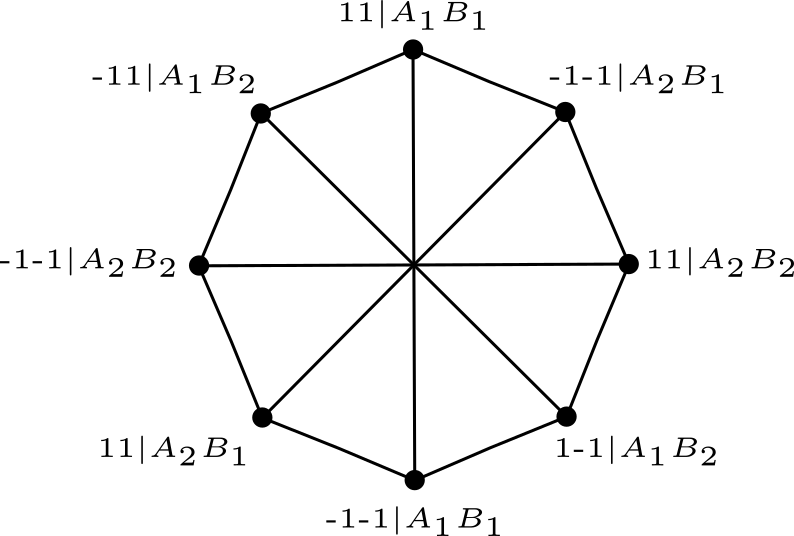
\includegraphics[width=0.6\textwidth]{images/chshexcl.png}
    \caption{Exclusivity graph for the CHSH correlations experiment, see Section \ref{sec:bell}. Like in Section \ref{sec:bell}, the outcomes of local measurements are labelled $\pm 1$. Vertices correspond to measurement events, exclusive measurement events are represented as adjacent.}
    \label{fig:chshexcl}
\end{figure}

The Lovász number of the CHSH exclusivity graph corresponds to the Tsirelson bound $B_q = \frac{1}{2}(1+\frac{1}{\sqrt{2}})$. Thus, the Lovász bound is tight and the measurements \ref{eqn:chshmnts}, together with the maximally entangled EPR state, produce a maximal violation of the CHSH inequality \ref{eqn:chshineq}. 

In fact, due to space-like separation, the Lovász bound is a tight upper bound that all correlations compatible with QM have to obey, even if we allow for general POVM measurements. This follows from the Naimark dilation theorem \cite{Watrous2018}. Informally, we can extend every non-projective quantum measurement $\{M_i\}_i$ acting on the system $\mathcal{A}$ to a projective measurement $\{\Pi_i^{\mathcal{A}}\}_i$ that acts on a composite system $(\thinspace\mathcal{A}+\text{ancilla}\thinspace)$, where the ancillary system is prepared in some well-defined state $\ket{0}\bra{0}$. The extended projectors acting on the composite system $(\thinspace\mathcal{A}+\text{ancilla}\thinspace)$ produce the same output correlations as the unsharp measurements acting on the single system $\mathcal{A}$. The same can be said about local measurements on subsystem $\mathcal{B}$. Now, due to space-like separation, the projectors $\Pi_i^{\mathcal{A}}\otimes \Pi_j^{\mathcal{B}}$ corresponding to exclusive measurement events commute. As such, we can follow the same line of reasoning as in Section \ref{sec:complicationscont} to argue that the maximal violation of the CHSH inequalitiy, even with access to unsharp measurements is given by the Tsirelson bound. As we saw in Section \ref{sec:complicationscont}, the same considerations do not apply to contextuality scenarios involving compatible measurements on a single system. While we can extend the individual measurements to projective measurements by adding an ancilliary system, thereby associating with each measurement event a projector, we have no grounds to assume that the projectors associated with exclusive measurement are orthogonal. Take for instance the KCBS correlation experiment with exclusivity graph Figure \ref{fig:kcbsexclusivity}. Measurements 1,2 and 2,3 are compatible, however not all three are jointly measurable. We can assume the Naimark projectors associated with the measurement events $0,1\thinspace\vert\thinspace 1,2$ and $0,0\thinspace\vert\thinspace 1,2$ to be orthogonal, because they correspond to distinct outcomes of a single joint measurements. This does not hold for the exclusive measurement events of the KCBS exclusivity graph: $0,1\thinspace\vert\thinspace 1,2$ and $0,1\thinspace\vert\thinspace 2,3$ can not be distinct outcomes of a single joint measurement, as the measurements $1,2,3$ are not even pairwise compatible.

Back to the CHSH correlation experiment: A violation of the CHSH inequality implies that the observed correlations are not compatible with a classical description of the form \ref{eqn:lhvm}, but require quantum resources, in particular entanglement, to generate. What is remarkable about, but not unique to the CHSH Bell inequality\footnote{Other Bell inequalities may self-test different reference experiments.}, is that the quantum model presented in \ref{eqn:chshmnts}, leading to a maximal violation of the inequality, i.e.\ corresponding to the extremal point $\Vec{v}_{max}\in\mathcal{Q}$ of the set of quantum correlations, see Figure \ref{fig:selftestingcorr}, is ``essentially unique". By this we mean that the only quantum model $\ket{\Psi}$, $\{\Pi_i\}_i$ predicting a maximal violation of the CHSH inequality is \ref{eqn:chshmnts}, modulo trivial changes to the reference experiment which we will specify shortly. A comprehensive proof is given in \cite{Supic2020}.
Thus, by interacting only classically with our preparation and measurement devices, we can characterize the quantum state and measurements our devices implement. We can only hope to self-test extremal correlations, as other correlations $\Vec{v}\in\mathcal{Q}$ correspond to a non-unique convex combination of distinct extremal correlations. 

It is apparent that we can never certify exact states and measurements, as we will always be blind to a number of trivial degrees of freedom. For instance, we cannot tell if there are any additional ancilliary systems, $\mathcal{A'}$, $\mathcal{B'}$, prepared in some joint state $\rho_{\mathcal{A'B'}}$, in the remote labs that we are not probing:
\begin{align*}
    & \ket{\Psi}_\mathcal{AB}\thinspace,\thinspace && A_{1} = \sigma_{z,\mathcal{A}}\otimes\mathbb{1}_{\mathcal{B}}\thinspace,\thinspace \dots \\
    \equiv\; & \ket{\Psi}\bra{\Psi}_{\mathcal{AB}}\otimes\rho_{\mathcal{A'B'}}\thinspace,\thinspace && A_1 = \sigma_{z,\mathcal{A}}\otimes\mathbb{1}_{\mathcal{A'BB'}}\thinspace,\thinspace\dots\; .
\end{align*}
Furthermore, we can never detect local unitaries $U=U_\mathcal{AA'}\otimes U_\mathcal{BB'}$, i.e.\ local basis changes:
\begin{align*}
    & \ket{\Psi}\bra{\Psi}_{\mathcal{AB}}\thinspace\otimes\thinspace\rho_{\mathcal{A'B'}}\thinspace,\thinspace && A_1 = \sigma_{z,\mathcal{A}}\thinspace\otimes\thinspace\mathbb{1}_{\mathcal{A'BB'}}\thinspace,\thinspace\dots \\ 
    \equiv\;  U(& \ket{\Psi}\bra{\Psi}_{\mathcal{A,B}}\thinspace\otimes\thinspace\rho_{\mathcal{A'B'}})U^{\dag}\thinspace,\thinspace && A_1 = U_{\mathcal{AA'}}(\sigma_{z,\mathcal{A}}\thinspace\otimes\thinspace\mathbb{1}_{\mathcal{A'BB'}})U_{\mathcal{AA'}}^{\dag}\thinspace,\thinspace\dots\; .
\end{align*}

According to Stinespring's Dilation Theorem \cite{Watrous2018}, these trivial degrees of freedom can account for arbitrary local isometries $\mathcal{A}\rightarrow\mathcal{AA'}$, $\mathcal{B}\rightarrow\mathcal{BB'}$. Furthermore, the previous two examples suggest that in order to define a sensible notion of self-testing, we must first define some notion of equivalence for quantum models. We then aim to construct self-testing protocols that single out a unique quantum model, modulo this notion of equivalence. This notion of equivalence should account for some trivial degrees of freedom, like the ones above, but should also not be too broad, in order for self-testing to be a powerful property of select correlation experiments. Ideally, the equivalence of quantum realizations should have an operational meaning. The following definition applies to Bell-type correlation experiments and does justice to these three criteria.

\begin{definition}[\cite{McKague2011}]
\label{def:equivexp}
A quantum experiment involving $\ket{\Psi'}_{\mathcal{A'B'P}}$ and local measurements $\{{P'}^{\thinspace a}_x\}_x$, $\{{Q'}^{\thinspace b}_y\}_y$, where $\ket{\Psi'}_{\mathcal{A'B'P}}$ is an arbitrary purification and ${P'}^{\thinspace a}_x$ is the positive semi-definite operator corresponding to the outcome $x$ of the local measurement $a$ on system $\mathcal{A}$, is \emph{equivalent} to a reference experiment $\ket{\Psi}_{\mathcal{AB}}, \{P_x^a\}_x$, $\{Q_y^b\}_y$, if there exists a local isometry $\Phi=\Phi_{\mathcal{A}}\otimes\Phi_{\mathcal{B}}$, $\Phi_{\mathcal{A/B}}\colon\mathcal{H}_{\mathcal{A'/B'}}\rightarrow\mathcal{H}_{\mathcal{A'/B'}}\otimes\mathcal{H}_{\mathcal{A/B}}$, such that
\begin{align*}
    (\Phi\otimes\mathbb{1}_{\mathcal{P}})\ket{\Psi'}_{\mathcal{A'B'P}} & =\ket{\text{junk}}_\mathcal{{A'B'P}}\otimes\ket{\Psi}_{\mathcal{AB}} \\[0.7em]
    (\Phi\otimes\mathbb{1}_{\mathcal{P}})({P'}^{\thinspace a}_x\otimes {Q'}^{\thinspace b}_y)\ket{\Psi'}_{\mathcal{A'B'P}} & =\ket{\text{junk}}_{\mathcal{A'B'P}}\otimes(P^a_x\otimes Q^b_y)\ket{\Psi}_{\mathcal{AB}} \thinspace .
\end{align*}
\end{definition}

Operationally, this means that a physical experiment is equivalent to some reference experiment if by means of local operations alone\footnote{Note that the two experimenters can realize an arbitrary local isometry $\Phi=\Phi_{\mathcal{A}}\otimes\Phi_{\mathcal{B}}$ by preparing ancilliary systems in some well-defined state $\ket{00}$ and subsequently applying local unitary operations.}, one can recover the reference experiment, up to some ``junk". In particular, the experimenters can for instance extract the reference state, i.e.\ the maximally entangled EPR state for the CHSH correlation experiment, to their ancilliary systems, by means of local operations alone. As local operations cannot generate entanglement, their initial state must have been maximally entangled. Note that the notion of equivalence, as defined in Definition \ref{def:equivexp}, is not an equivalence relation, as it fails to be symmetric \cite{McKague2011}.  While the experimenters can extract the reference state to ancilliary systems using only local operations, if they have access to an equivalent experiment, the converse direction must not hold: Consider the reference CHSH experiment \ref{eqn:chshmnts} producing a maximal violation of the CHSH inequality \ref{eqn:chshineq}. Further, consider the equivalent quantum experiment where both experimenters control an additional ancilliary system and both ancillae are prepared in an entangled state. While this extended experiment is equivalent to the reference experiment, the converse does not hold, as we cannot create entanglement by local operations alone.

Definition \ref{def:equivexp} accounts for all of the following statistics-preserving trivial degrees of freedom, as presented in \cite{McKague2011}:
\begin{enumerate}
    \item Local changes of basis
    \item adding ancillae to the physical systems, prepared in any joint state (measurements do not act on these)
    \item changing the action of an observable outside the support of the state
    \item locally embedding the state and operators into a larger (or smaller) Hilbert space
\end{enumerate}

\begin{claim}[\cite{McKague2011}]
Any finite number of changes 1-4 transforms a quantum experiment into an equivalent quantum experiment like in Definition \ref{def:equivexp}. Furthermore, any quantum experiment equivalent to some reference experiment can be constructed from that reference experiment by applying  a finite number of changes 1-4.
\end{claim}

Let us constrast self-testing via Bell inequalities with self-testing via KS non-contextuality inequalities. Section \ref{sec:contselftesting} will examine in detail a self-testing protocol based on the class of odd $n$-cycle KS non-contextuality inequalities \cite{Bharti2019}. Importantly, without space-like separated subsystems, we have to give up device-independence: While relaxing the assumption of space-like separation means that we no longer require the device to be split up among remote subsystems, or that it can generate a large number of entangled states, we can no longer make use of quantum non-locality to certify that the correlations were not simulated by some pre-programmed classical computer \cite{Supic2020}. In principle, we can never discard this possibility without imposing additional assumptions about the devices. In Section \ref{sec:memoryass}, we examine how bounding the information carrying capacity or memory of the device can be helpful in this regard. Additionally, the CSW framework in Section \ref{sec:csw}, which gives us non-trivial constraints on the set of valid quantum models, which we will be use in the self-testing proof, requires assumptions about operator compatibility and sharpness. This is illustrated in Figure \ref{fig:selftesting}. Since contextuality scenarios no longer require remote subsystems, we need to amend our notion of ``equivalence" for quantum experiments, see Definition \ref{def:equivexp}, accordingly. We will come back to this in Section \ref{sec:contselftesting}, but already note that contextuality-based self-testing protocols aim to single out a quantum realization, up to a \textbf{global} isometry.

Finally, self-testing results should be robust to noise. Informally, this means that a near-optimal violation of the Bell or KS non-contextuality inequality should imply that all compatible quantum models are, up to equivalence, ``close" to the reference quantum experiment. The self-testing protocol we will examine in Section \ref{sec:contselftesting} is robust, see Theorem \ref{thm:contselftesting}.

\begin{figure}
    \centering
    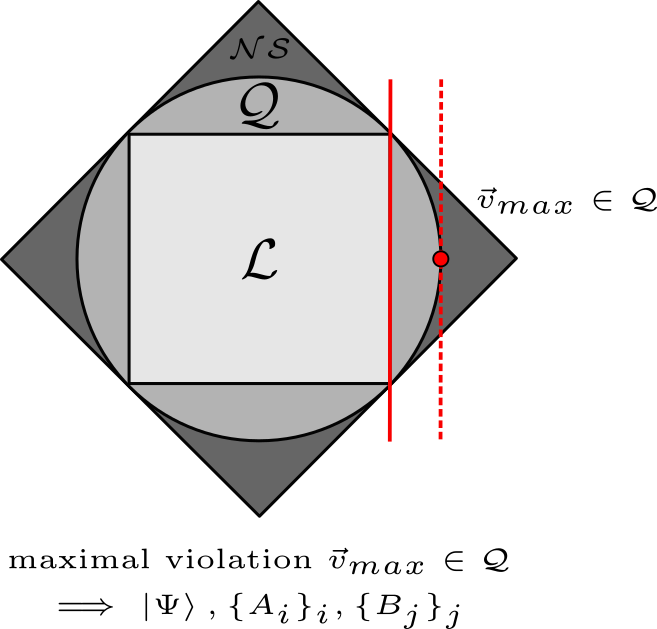
\includegraphics[width=0.6\textwidth]{images/self-testingcorr.png}
    \caption{Schematic drawing depicting the geometry of the convex sets $\mathcal{L}$, $\mathcal{Q}$, and $\mathcal{NS}$, containing all local, quantum, and no-signalling correlations, respectively. A Bell inequality, like the CHSH inequality, defines a separative hyperplane such that all local correlations $\mathcal{L}$ lie to one ``side" of this hyperplane, here represented by the unbroken red line. The extremal point(s) $\Vec{v}_{max}\in\mathcal{Q}$ of the set of quantum correlations $\mathcal{Q}$ corresponds to a maximal violation of the CHSH inequality. The CHSH inequality can be used for self-testing, as the quantum model $\ket{\Psi}$,$\{\Pi_i\}_i$ compatible with a maximal violation of the inequality is unique, up to trivial degrees of freedom.}
    \label{fig:selftestingcorr}
\end{figure}

\begin{figure}
    \centering
    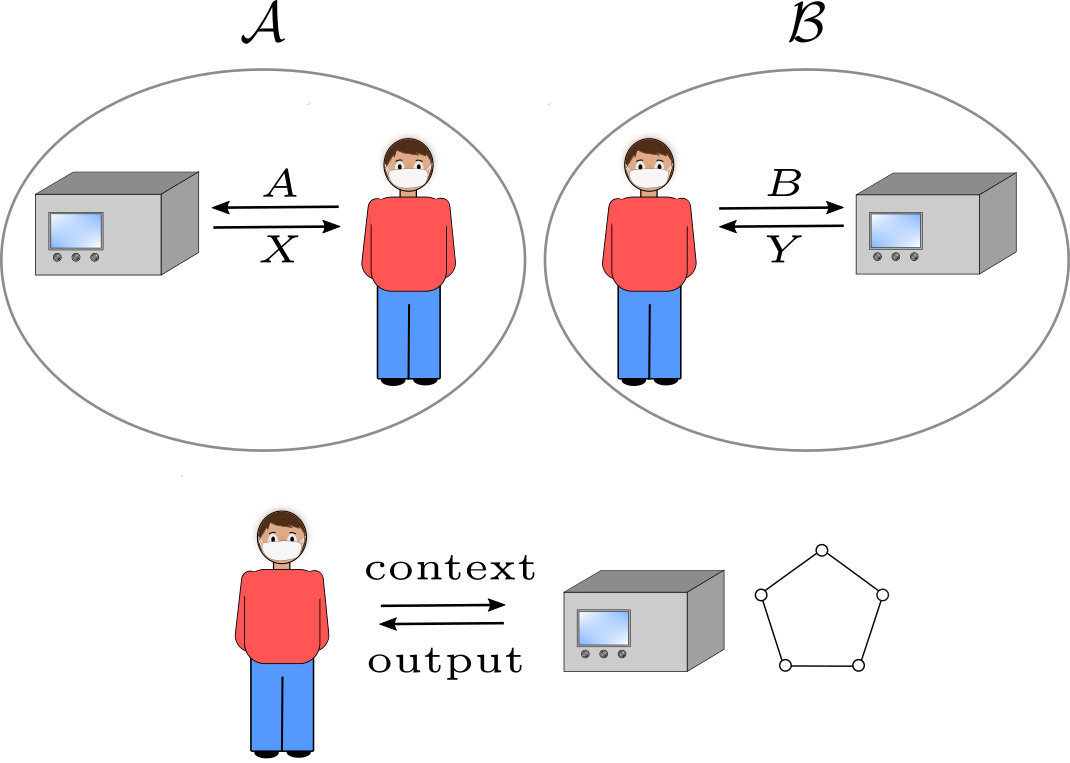
\includegraphics[width=0.8\textwidth]{images/self-testing.png}
    \caption{\textbf{Top}: Typical device-independent Bell-type self-testing scenario. The two subsystems $\mathcal{A}$ and $\mathcal{B}$ are space-like separated. Accordingly, the black box device, which can be interpreted as a correlation experiment testing a Bell inequality, is split into two non-communicating parts. An experimenter can interact classically with a local sub-device, by passing an input value and recording the outcome returned by the device. A violation of the tested Bell inequality implies that the corresponding correlations were obtained by quantum means, i.e.\ joint measurements on an entangled state shared between $\mathcal{A}$, $\mathcal{B}$. For some Bell inequalities, a maximal violation is only compatible with an essentially unique quantum realization, i.e.\ quantum state and set of measurements.
    \textbf{Bottom:} In contrast, self-testing protocols based on KS non-contextuality inequality violations do not assume the device to be split into multiple non-communicating parts. Instead, a single experimenter interacts classically with the device by freely choosing between measurement contexts and determining the corresponding outcome probabilities. Dropping the unnatural assumption of space-like separation complicates the problem of self-testing considerably and we are required to make additional assumptions about the device, for example regarding compatibility relations and information carrying capacity. Thus, contextuality-based self-testing protocols are only semi-device-independent.}
    \label{fig:selftesting}
\end{figure}

\chapter{Self-testing via KS non-contextuality inequalities}
\lhead{\emph{Self-testing via KS non-contextuality inequalities}}
\label{sec:contselftesting}

\section{Preceding results}

In Section \ref{sec:csw}, we considered general correlation experiments testing some linear combination of probabilities $S$ and found that any quantum realization $\ket{\Psi}$, $\Pi_i$ can be translated into a feasible solution $X$ of the Lovász SDP \ref{eqn:lovaszsdp}, such that the value of $S$, as predicted by QM, corresponds to the objective function the SDP aims to maximize, evaluated at the feasible solution $X$. Conversely, if there are no additional physical constraints, for example due to space-like separated subsystems, one can construct a quantum realization for every feasible solution $X$ that achieves $S=\sum_{i=1}^n X_{ii}$. Such quantum realization was constructed from an arbitrary Gram decomposition of $X$. This connection between feasible solutions to the Lovász SDP and quantum models of the correlation experiment will be central to proving robust self-testing based on KS non-contextuality inequalities.

As outlined in Section \ref{sec:self-testing}, the essence of self-testing is that a maximal violation of suitable Bell or KS non-contextuality inequalities is only compatible with an essentially unique quantum realization $\ket{\Psi}$, $\{\Pi_i\}_i$, up to statistics-preserving trivial degrees of freedom. Furthermore, the inequalities are tests of non-classicality. If our experiment produces correlations that violate these, this certifies that the correlations were not simulated by some classical mechanism, which would render all proofs of information-theoretic security superfluous. Extra care has to be taken in the case of contextuality scenarios, as will be the topic of Section \ref{sec:memoryass}. Ideally, such self-tests should be robust to noise, i.e.\ a $\epsilon$-suboptimal violation should imply that the only compatible quantum realizations are ``close" to the ideal reference implementation, up to trivial degrees of freedom.

We will now sketch the proof in \cite{Bharti2019}, which demonstrates that the class of odd $n$-cycle contextuality scenarios allows for robust self-testing. Recall that an odd $n$-cycle correlation experiment assumes cyclic compatibility relations, like in Figure \ref{fig:kcbscompat}. The self-testing protocol consists of an experimenter choosing freely between the $n$ measurement contexts $(i,i\oplus1)$ and determining the outcome correlations $p(0,1\thinspace\vert\thinspace i,i\oplus 1)$ that constitute the test $S$. The main ``ingredients" of the proof are the following three lemmas:

\begin{lemma}[\cite{Bharti2019}]
\label{lem:kcbsunique}
For the class of odd $n$-cycle exclusivity graphs, $n\geq5$, the Lovász SDP \ref{eqn:lovaszsdp} has a unique optimal solution $X^*_n$.   
\end{lemma}

From Section \ref{sec:cswhierarch} we know that the reference quantum experiment $\{\vert u_j^{(n)} \rangle \}_{j=0}^{n}$ presented in Section \ref{sec:kcbs} produces a maximal violation of the odd $n$-cycle KS non-contextuality inequality, because it attains the Lovász bound. The unique optimal solution $X^*_n$ is obtained from this reference quantum realization by the usual procedure:
\begin{equation*}
    X^*_n=\operatorname{Gram}(\thinspace\vert u_0 \rangle\thinspace,\thinspace \langle u_1^{(n)} \vert u_0 \rangle \vert u_1^{(n)} \rangle\thinspace,\thinspace\dots,\thinspace \langle u_n^{(n)} \vert u_0 \rangle \vert u_n^{(n)} \rangle\thinspace)\thinspace.
\end{equation*}

The following two lemmas will be important to prove robustness:

\begin{lemma}[\cite{Bharti2019}]
\label{lem:epssuboptgram}
Let $(\mathcal{G}_{ex},w)$ be a weighted exclusivity graph with $n$ vertices and assume that \ref{eqn:lovaszsdp} has a unique optimal solution $X^*\in \mathcal{S}_+^{\thinspace n+1}$. Further, let $\Tilde{X}$ be a feasible solution of \ref{eqn:lovaszsdp} that is $\epsilon$-suboptimal, i.e.\
\begin{equation*}
    \sum_{i=1}^n w_i\thinspace\Tilde{X}_{ii} \geq B_{q}(\mathcal{G}_{ex},w)-\epsilon,
\end{equation*}
where $B_{q}(\mathcal{G}_{ex},w)=\sum_{i=1}^n w_i X_{ii}^*$ is the optimal solution of the Lovász SDP for the weighted exclusivity graph $(\mathcal{G}_{ex},w)$.
Then
\begin{equation*}
\|\Tilde{X}-X^*\|_F \leq \mathcal{O}(\epsilon)\,,
\end{equation*}
where $\|A\|_F=\operatorname{tr}(A^{\dag}A)$ is the Frobenius norm.
\end{lemma}

\begin{lemma}
\label{lem:closegramdecomp}
Let $\Tilde{X}\in S_{+}^{\thinspace n+1}$ be a positive semi-definite matrix, $\epsilon$-close to $X^*\in S_{+}^{\thinspace n+1}$ like in \ref{lem:kcbsunique}
\begin{equation*}
\|\Tilde{X}-X^*\|_F \leq \epsilon.
\end{equation*}
Let $\{\vert \Tilde{u}_i \rangle\}_{i=0}^n\subset\mathbb{C}^{d}$ and $\{\vert u_i\rangle\}_{i=0}^n\subset\mathbb{C}^{d}$ be Gram decompositions of $\Tilde{X}$ and $X^*$, respectively. Then there exists a $d\times d$ unitary matrix $U$ such that for all $i\in\{0,\dots,n\}$
\begin{equation*}
    \|\vert \Tilde{u}_i\rangle - U \vert u_i\rangle\|_2 \leq \kappa(n)\epsilon + \mathcal{O}(\kappa(n)^2\epsilon^2)\,,¸
\end{equation*}
where $\kappa(n)=\frac{1}{2}\sqrt{n+4}$ for all $n>7$.
\end{lemma}

We will omit the proofs of Lemmas \ref{lem:kcbsunique} and \ref{lem:epssuboptgram}, as they do not provide much conceptual insight, and offer only a few comments. We include the proof of Lemma \ref{lem:closegramdecomp}, as \cite{Bharti2019} proves only a weaker version, in the sense that $d=n$. Furthermore, the proof we present establishes a tighter error bound of the order $\mathcal{O}(\kappa(n)\epsilon)$, compared to $\mathcal{O}(\sqrt{(n+1)\epsilon}\,)$ in \cite{Bharti2019}. As opposed to the result in \cite{Bharti2019}, the proof of Lemma \ref{lem:closegramdecomp} makes use of the fact that the verifier has knowledge about the ideal Gram matrix $X^*$. 

The proof of Lemma \ref{lem:kcbsunique} utilizes SDP duality theory and shows a sufficient condition for the unicity of $X^*_n$ to be satisfied by explicit construction. It applies only to the class of odd $n$-cycle scenarios, as it makes use of the cyclic exclusivity constraints that enter the Lovász SDP \ref{eqn:lovaszsdp}. Lemma \ref{lem:epssuboptgram} is a general result for the optimization problem \ref{eqn:lovaszsdp}, and as such applies to arbitrary exclusivity graphs. Like Lemma \ref{lem:kcbsunique}, the proof of Lemma \ref{lem:epssuboptgram} makes heavy use of SDP duality theory. 

\begin{proof}\emph{(of Lemma \ref{lem:closegramdecomp})}\hfill\break
The proof is a generalization of the proof of Theorem 7.3.11 in \cite{Horn2013}, which only considers the noise-less case $\epsilon=0$, and we for the most part will adopt their notation. 

Define $A$, $B$ $\in\mathbb{C}^{n+1,d}$ as the matrices with rows $\{\vert u_i\rangle\}_{i=0}^n\subset\mathbb{C}^{d}$ and $\{\vert \Tilde{u}_i \rangle\}_{i=0}^n\subset\mathbb{C}^{d}$, respectively. The Gram matrices $\Tilde{X}$ and $X^*$ are given by $X^*=AA^{\dag}$ and $\Tilde{X}=BB^{\dag}$. 

Let $A^\dag = V\Sigma W^\dag$ be a singular value decomposition (SVD) of $A^\dag$, $V\in\mathbb{C}^{d,d}$ and $W\in\mathbb{C}^{n+1,n+1}$ being unitary matrices, and $\Sigma$ a rectangular diagonal matrix containing the singular values of $A^\dag$. By definition, 
\begin{equation*}
X^*=AA^\dag=(A^\dag)^{\dag} A^{\dag} = W\Sigma^\dag\Sigma W^\dag = W\Lambda W^\dag,
\end{equation*} where we have defined $\mathbb{C}^{n+1,n+1}\ni\Lambda\coloneqq\Sigma^\dag\Sigma$. Denote the non-zero singular values of $A^\dag$, ordered according to magnitude, by $\sigma_1 \geq \dots \geq \sigma_r > 0$, where $r$ is the rank of $A^\dag$. Note that $A$ and $A^{\dag}$ have identical singular values. As acting with permutation matrices on $V$, $W^{\dag}$ preserves unitarity, we can w.l.o.g\ assume
\begin{equation*}
\Lambda = 
\begin{pmatrix}
\sigma_1^2 & & & \\
& \ddots & & \\
& & \sigma_r^2 & \\
& & & 0_{n+1-r}\\
\end{pmatrix},
\end{equation*}
where empty spaces indicate zero entries.
Further, let
\begin{equation*}
\Sigma_r = 
\begin{pmatrix}
\sigma_1 & &\\
& \ddots & & \\
& & \sigma_r\\
\end{pmatrix}\in\mathbb{C}^{r,r}
\end{equation*} and partition $W\in\mathbb{C}^{n+1,n+1}$ like 
$\begin{pmatrix}
W_1 & W_2
\end{pmatrix}$, with $W_1\in\mathbb{C}^{n+1,r}$ and $W_2\in\mathbb{C}^{n+1,n+1-r}$. Theorem 7.3.2 in \cite{Horn2013} implies that there exists an isometry $V_1\in\mathbb{C}^{d,r}$ such that 
\begin{equation*}
A^{\dag}=V_1\Sigma_r W_1^{\dag}.
\end{equation*}
The first step towards proving Lemma \ref{lem:closegramdecomp} is to generalize the result of Theorem 7.3.2 in \cite{Horn2013}. Concretely, we want to show that $B^{\dag}$, obeying $(B^{\dag})^{\dag}B^{\dag}\approx X^* = W\Lambda W^{\dag}$, can be approximately written like $B^{\dag}\approx V_2\Sigma_rW_1^{\dag}$, where $V_2\in\mathbb{C}^{d,r}$ is an isometry.

By definition,
\begin{equation*}
(B^{\dag})^{\dag}B^{\dag}=\Tilde{X}\stackrel{\epsilon}{\approx}X^*=W\Lambda W^{\dag}.
\end{equation*}
Let 
\begin{equation*}
D\coloneqq\Sigma_r\oplus\mathbb{1}_{n+1-r}\in\mathbb{C}^{n+1,n+1}
\end{equation*} be the $(n+1)\times (n+1)$ diagonal matrix with diagonal entries corresponding to the non-zero singular values of $A^{\dag}$. The remaining $n+1-r$ diagonal entries are set to $1$, such that $D$ is invertible. Further, define
\begin{equation*}
X\coloneqq B^{\dag} W D^{-1}\in\mathbb{C}^{d,n+1}.
\end{equation*}
We partition $X$ like $X=
\begin{pmatrix}
\Tilde{V_2} &  Z
\end{pmatrix}$, where $\Tilde{V_2}\in\mathbb{C}^{d,r}$.
It follows that
\begin{alignat*}{2}
X^{\dag}X & = D^{-1}W^{\dag}BB^{\dag}WD^{-1} && \\[0.2em]
& = D^{-1}W^{\dag}AA^{\dag}WD^{-1} && +D^{-1}W^{\dag}(BB^{\dag}-AA^{\dag})WD^{-1} \\[0.2em]
& = D^{-1}\Lambda D^{-1} && + D^{-1}W^{\dag}(\Tilde{X}-X^*)WD^{-1} \\[0.2em]
& =
\begin{pmatrix}
\mathbb{1}_r & \\
& 0_{n-r}
\end{pmatrix} && + D^{-1}W^{\dag}(\Tilde{X}-X^*)WD^{-1}.
\end{alignat*}
Therefore,
\begin{equation*}
X^{\dag}X=
\begin{pmatrix}
\Tilde{V}_2^{\dag}\\
Z^{\dag}
\end{pmatrix}
\begin{pmatrix}
\Tilde{V}_2 & Z
\end{pmatrix} =
\begin{pmatrix}
\Tilde{V}_2^{\dag}\Tilde{V}_2 & \Tilde{V}_2^{\dag} Z \\
Z^{\dag}\Tilde{V}_2 & Z^{\dag}Z
\end{pmatrix}
= 
\begin{pmatrix}
\mathbb{1}_r & \\
& 0_{n+1-r}
\end{pmatrix} + D^{-1}W^{\dag}(\Tilde{X}-X^*)WD^{-1}.
\end{equation*}
Next, we aim to bound the Frobenius distance
\begin{equation*}
\left\|
\begin{pmatrix}
\Tilde{V}_2^{\dag}\Tilde{V}_2 & \Tilde{V}_2^{\dag} Z \\
Z^{\dag}\Tilde{V}_2 & Z^{\dag}Z
\end{pmatrix}
-
\begin{pmatrix}
\mathbb{1}_r & \\
& 0_{n+1-r}
\end{pmatrix}
\right\|_F.
\end{equation*}
Unitaries leave the Frobenius norm invariant, as $\|A\|_F^{\textstyle ^2}=\sum_k\|Ae_k\|_2^{\textstyle ^2} = \sum_k \|UAe_k\|_2^{\textstyle ^2}=\|UA\|_F^{\textstyle ^2}\thinspace$, where $U$ is a unitary. We find:
\begin{align*}
\left\|
\begin{pmatrix}
\Tilde{V}_2^{\dag}\Tilde{V}_2 & \Tilde{V}_2^{\dag} Z \\
Z^{\dag}\Tilde{V}_2 & Z^{\dag}Z
\end{pmatrix}
-
\begin{pmatrix}
\mathbb{1}_r & \\
& 0_{n-r}
\end{pmatrix}
\right\|_F\;=\;\|WD^{-1}W^{\dag}(\Tilde{X}-X^*)WD^{-1}W^{\dag}\|_F\; & \leq\; \epsilon\thinspace \operatorname{max}\left\{\sigma_{\text{min}}^{(n)}{}^{-2},1\right\}\\ & =\epsilon\thinspace\operatorname{max}\left\{\lambda_{\text{min}}^{(n)}{}^{-1},1\right\},
\end{align*}
where $\sigma_{\text{min}}^{(n)}$ is the non-zero singular value of $A$ with smallest magnitude, the square of which is the smallest non-zero eigenvalue of $X^*$, $\lambda_{\text{min}}^{(n)}$.
For the KCBS scenario, $n=5$, we find $\lambda_{\text{min}}^{(n)}=\frac{1}{2}(\sqrt{5}-1)\approx 0.618$.

Therefore,
\begin{alignat*}{2}
\|\Tilde{V}_2^{\dag}\Tilde{V}_2-\mathbb{1}_r\|_F & \stackrel{(\triangle)}{\leq}\epsilon\thinspace \operatorname{max}\left\{\lambda_{\text{min}}^{(n)}{}^{-1},1\right\} &&\text{ and}\\[0.5em]
\|Z\|_F & \stackrel{(\square)}{\leq}\epsilon\thinspace\operatorname{max}\left\{\lambda_{\text{min}}^{(n)}{}^{-1},1\right\}+&&\thinspace\mathcal{O}(\epsilon^2\operatorname{max}\left\{\lambda_{\text{min}}^{(n)}{}^{-1},1\right\}^2)\thinspace,
\end{alignat*}
where $(\square)$ follows from $(\triangle)$, as we will show. For now, let us assume $(\square)$ to be true.

By definition, $X=B^{\dag}WD^{-1}$, and hence
\begin{equation*}
B^{\dag}=XDW^{\dag} = 
\begin{pmatrix}
\Tilde{V}_2 & Z
\end{pmatrix}
\begin{pmatrix}
\Sigma_r &\\
& \mathbb{1}_{n-r}
\end{pmatrix}
\begin{pmatrix}
W_1^{\dag} \\ W_2^{\dag}
\end{pmatrix} = 
\begin{pmatrix}
\Tilde{V}_2 \Sigma_r & Z
\end{pmatrix}
\begin{pmatrix}
W_1^{\dag} \\ W_2^{\dag}
\end{pmatrix} = \Tilde{V}_2\Sigma_r W_1^{\dag} + ZW_2^{\dag}
\end{equation*}
Therefore,
\begin{equation*}
\|B^{\dag}-\Tilde{V}_2\Sigma_r W_1^{\dag}\|_F=\|ZW_2^{\dag}\|_F=\|Z\|_F\leq \epsilon\thinspace \operatorname{max}\left\{\lambda_{\text{min}}^{(n)}{}^{-1},1\right\}+\mathcal{O}(\epsilon^2\operatorname{max}\left\{\lambda_{\text{min}}^{(n)}{}^{-1},1\right\}^2).
\end{equation*}
Crucially, $\Tilde{V}_2$ is approximately isometric, which follows from the previously derived bound on $\|\Tilde{V}_2^{\dag}\Tilde{V}_2 -\mathbb{1}_r\|_F$, as we will now prove:

Consider a SVD of $\Tilde{V}_2$,
\begin{equation*}
\Tilde{V}_2 = S\Tilde{\Sigma}T^{\dag},
\end{equation*} and define $V_2$ as the isometry
\begin{equation*}
V_2\coloneqq S \begin{pmatrix} \mathbb{1}_r \\ 0_{d-r,r} \end{pmatrix} T^{\dag}.
\end{equation*} $V_2$ is isometric because
\begin{equation*}
V_2^{\dag}V_2=T\begin{pmatrix} \mathbb{1}_r & 0_{r,d-r} \end{pmatrix} \begin{pmatrix} \mathbb{1}_r \\ 0_{d-r,r} \end{pmatrix} T^{\dag}=T\thinspace \mathbb{1}_r \thinspace T^{\dag} = \mathbb{1}_r,
\end{equation*}
and its Frobenius distance to $\Tilde{V}_2$ is
\begin{equation*}
\|\Tilde{V}_2-V_2\|_F^{\textstyle ^2} = \left\|S\left[\Tilde{\Sigma}-\begin{pmatrix}
\mathbb{1}_r \\ 0_{d-r,r}\end{pmatrix}\right]T^{\dag}\right\|_F^2=\operatorname{tr}\left(\left[\Tilde{\Sigma}^{\dag}-\begin{pmatrix} \mathbb{1}_r & 0_{r,d-r}\end{pmatrix}\right]\left[\Tilde{\Sigma}-\begin{pmatrix} \mathbb{1}_r \\ 0_{d-r,r}\end{pmatrix}\right]\right)
\end{equation*}
Let $r'$ be the rank of $\Tilde{V}_2$, and $\Tilde{\sigma_1}\geq\dots\Tilde{\sigma}_{r'}>0$ the non-zero singular values of $\Tilde{V}_2$. Again, w.l.o.g.\
\begin{equation*}
\Tilde{\Sigma}^{\dag}=
\begin{pmatrix}
\Tilde{\sigma}_1 &&& \\
&\ddots&& \\
&&\Tilde{\sigma}_{r'}& \\
&&&0_{r-r'}\\[0.1em]
\multicolumn{4}{c}{0_{d-r,r}}
\end{pmatrix}.
\end{equation*}
Hence, $\|\Tilde{V}_2-V_2\|_F$ can be re-written like
\begin{align*}
\|\Tilde{V}_2-V_2\|_F^{\textstyle ^2} & =\operatorname{tr}\left(
\begin{pmatrix}
\Tilde{\sigma}_1^2&&&\\
&\ddots&&\\
&&\Tilde{\sigma}_{r'}^2&\\
&&& 0_{r-r'}
\end{pmatrix} -2
\begin{pmatrix}
\Tilde{\sigma}_1&&&\\
&\ddots&&\\
&&\Tilde{\sigma}_{r'}&\\
&&& 0_{r-r'}
\end{pmatrix}+\mathbb{1}_r\right)\\[0.5em] &  =\sum_{i=1}^{r'}(\Tilde{\sigma}_i^2-2\Tilde{\sigma}_i+1) + (r-r') =\sum_{i=1}^{r'}(\Tilde{\sigma}_i-1)^2+(r-r').
\end{align*}
The condition $\|\Tilde{V}_2^{\dag}\Tilde{V}_2 -\mathbb{1}_r\|_F\leq\epsilon\thinspace\operatorname{max}\left\{\lambda_{\text{min}}^{(n)}{}^{-1},1\right\}$ implies
\begin{align*}
\left\|T
\begin{pmatrix}
\Tilde{\sigma}_1^2&&& \\
&\ddots&& \\
&&\Tilde{\sigma}_{r'}^2& \\
&&&0_{r-r'}
\end{pmatrix}T^{\dag}-\mathbb{1}_r\right\|_F^2 & =\sum_{i=1}^{r'}(\Tilde{\sigma}_i^4-2\Tilde{\sigma}_i^2+1) + (r-r') \\
& = \sum_{i=1}^{r'}(\Tilde{\sigma}_i-1)^2(\Tilde{\sigma}_i+1)^2 + (r-r')\leq \epsilon^2\operatorname{max}\left\{\lambda_{\text{min}}^{(n)}{}^{-1},1\right\}^2\;,
\end{align*}
which in particular implies that, for $\epsilon<\operatorname{min}\left\{\lambda_{\text{min}}^{(n)},1\right\}$, the rank of $\Tilde{V}_2$ must match that of $A^{\dag}$, i.e. $r=r'$. Additionally, $\Tilde{V}_2$ is approximately isometric:
\begin{equation*}
\|\Tilde{V}_2-V_2\|_F^{\textstyle ^2} = \sum_{i=1}^r(\Tilde{\sigma_i}-1)^2\leq\epsilon^2\operatorname{max}\left\{\lambda_{\text{min}}^{(n)}{}^{-1},1\right\}^2\thinspace.
\end{equation*}
Together, this gives us the desired intermediate result:
\begin{align*}
\|B^{\dag}-V_2\Sigma_r W_1^{\dag}\|_F\leq \|B^{\dag}-\Tilde{V_2}\Sigma_r W_1^{\dag}\|_F + \|(\Tilde{V}_2-V_2)\Sigma_r W_1^{\dag}\|_F \leq & \thinspace\epsilon\thinspace\operatorname{max}\left\{\lambda_{\text{min}}^{(n)}{}^{-1},1\right\}(1+\sigma_{\text{max}}^{(n)})\thinspace \\ & + \mathcal{O}(\epsilon^2\operatorname{max}\left\{\lambda_{\text{min}}^{(n)}{}^{-1},1\right\}^2),
\end{align*}
where $\sigma_{\text{max}}^{(n)}$ is the maximum singular value of $A^{\dag}$. We take the second term to be negligible. For the KCBS scenario, $n=5$, $\sigma_{\text{max}}^{(n)}=\sqrt{2}$, and consequently $\|B^{\dag}-V_2\Sigma_r W_1^{\dag}\|_F\leq \kappa\epsilon$, where $\kappa \approx 3.55$. 
For $n>7$, one finds numerically that $\operatorname{max}\left\{\lambda_{\text{min}}^{(n)}{}^{-1},1\right\}=1$. Additionally, $\lambda_{\text{max}}^{(n)}=\sigma_{\text{max}}^{(n)}{}^2$ scales linearly in $n$ like $\lambda_{\text{max}}^{(n)}\approx \frac{1}{4}n+1$.

To recap, we have just shown that
\begin{align*}
A^{\dag} & =V_1\Sigma_r W_1^{\dag} \\[0.3em]
B^{\dag} & \stackrel{\mathcal{O}(\kappa(n)\epsilon)}{\approx} V_2\Sigma_r W_1^{\dag},
\end{align*}
where $V_2$ is an isometry. The next proof step is to show that there exists a unitary $U\in\mathbb{C}^{d,d}$ such that $B^{\dag}\approx U A^{\dag}$.

According to Theorem 2.1.18 in \cite{Horn2013}, there exists a unitary $U\in\mathbb{C}^{d,d}$ such that $V_2=UV_1$. This unitary $U$ also relates the matrices $B^{\dag}$ and $A^{\dag}$, as
\begin{equation*}
B^{\dag}\stackrel{\mathcal{O}(\kappa(n)\epsilon)}{\approx}V_2\Sigma_r W_1^{\dag}= UV_1\Sigma_r W_1^{\dag}=UA^{\dag}.
\end{equation*} 
Finally, we can use this result to bound the distance between the two Gram decompositions $\{u_i\}_{i=0}^n$ and $\{\Tilde{u}_i\}_{i=0}^n$, and thereby conclude the proof:
\begin{align*}
\|B^{\dag}-UA^{\dag}\|_F&=\|
\begin{pmatrix}
\Tilde{u}_1 \;| & \dots & |\; \Tilde{u}_n
\end{pmatrix}-U
\begin{pmatrix}
u_1 \;| & \dots &  | \; u_n
\end{pmatrix} \|_F \\[0.3em]
& = \|
\begin{pmatrix}
\Tilde{u}_1-U u_1\; | &\dots& |\;\Tilde{u}_n-U u_n
\end{pmatrix}
\|_F\leq\kappa(n)\epsilon + \mathcal{O}(\kappa(n)^2\epsilon^2),
\end{align*}
where vertical lines delimit columns.
Since the Frobenius norm of an $n\times m$ matrix is just the two norm of the $(n\cdot m)$-long vector containing all matrix entries, we have
\begin{equation*}
\forall i\in\{0,\dots,n\}: \|\vert\Tilde{u}_i\rangle-U\vert u_i\rangle\|_2 \leq \kappa(n)\epsilon + \mathcal{O}(\kappa(n)^2\epsilon^2).
\end{equation*}
The only thing that remains is proving the inequality $(\square)$. By considering the off-diagonal entries of $X^{\dag}X$, we find that
\begin{equation*}
\epsilon\thinspace\lambda_{\text{min}}^{(n)}{}^{-1} \geq \|Z^{\dag}\Tilde{V}_2\|_F=\|Z^{\dag}V_2 - Z^{\dag}(V_2-\Tilde{V}_2)\|_F.
\end{equation*}
The reverse triangle inequality and submultiplicativity of the Frobenius norm yields
\begin{equation*}
\epsilon\thinspace\lambda_{\text{min}}^{(n)}{}^{-1} \geq \|Z^{\dag}V_2\|_F - \|Z^{\dag}(V_2-\Tilde{V}_2)\|_F \geq \|Z\|_F(1-\|V_2-\Tilde{V}_2\|_F),
\end{equation*}
which implies
\begin{equation*}
\|Z\|_F \leq \epsilon\thinspace\lambda_{\text{min}}^{(n)}{}^{-1} + \mathcal{O}(\epsilon^2\lambda_{\text{min}}^{(n)}{}^{-2})\thinspace.
\end{equation*}
\end{proof}

Note that Lemma \ref{lem:closegramdecomp} is of no use for Bell-type self-testing scenarios, as it relates two Gram decompositions only by a global unitary $U$.

Having distilled the main proof components into three auxiliary theorems, Lemmas \ref{lem:kcbsunique}-\ref{lem:closegramdecomp}, we will now demonstrate that these imply the desired self-testing result. \cite{Bharti2019} for the most part omits these final proof steps. Section \ref{sec:kscontass} will provide an in-depth discussion about all of the assumptions that go into the self-testing protocol.

\begin{theorem}[Odd $n$-cycle KS non-contextuality inequalities facilitate self-testing \cite{Bharti2019}]
\label{thm:contselftesting}\hfill\break
Let $n\geq5$ be an odd integer. The only quantum model $\ket{\Psi}$, $\{\Pi_i\}_{i=1}^n$ compatible with a maximal violation of the odd $n$-cycle KS non-contextuality inequality \ref{eqn:oddncycleclass} with exclusivity graph $\mathcal{G}_{ex}^{(n)}$ is \ref{eqn:ncycleideal}, up to a global isometry:
\begin{align*}
    \exists \emph{ isometry } V & : \ket{\Psi} = V \vert u_0\rangle \\[0.7em]
    \forall i\in\{1,\dots,n\} & : \Pi_i \ket{\Psi} = V \vert u_i^{(n)} \rangle \langle u_i^{(n)} \vert \thinspace \vert u_0 \rangle
\end{align*}

Furthermore, all quantum models $\ket{\Psi}$, $\{\Pi_i\}_{i=1}^n$ compatible with an $\epsilon$-suboptimal violation of \ref{eqn:oddncycleclass}, i.e.\
\begin{equation*}
    \sum_{i=0}^n \abs{\langle \Psi \vert \Pi_i \vert \Psi \rangle}^2> B_q(\mathcal{G}_{ex}^{(n)})-\epsilon\thinspace ,
\end{equation*}where $B_q(\mathcal{G}_{ex}^{(n)})$ is the quantum supremum \ref{eqn:ncyclequsup}, are $\mathcal{O}(\epsilon)$ close in 2-norm to \ref{eqn:ncycleideal}, up to a global isometry:
\begin{align*}
    \exists \emph{ isometry } V & : \| \ket{\Psi} - V \vert u_0\rangle \|_2 \thinspace\leq\thinspace \mathcal{O}(\epsilon)\\[0.7em]
    \forall i\in\{1,\dots,n\} & : \| \Pi_i \ket{\Psi} - V \vert u_i^{(n)} \rangle \langle u_i^{(n)} \vert \thinspace \vert u_0 \rangle \| \leq \mathcal{O}(\epsilon)
\end{align*}
\end{theorem}

Here, the global isometry $V$ expresses the fact that the statistics of a correlation experiment are always blind to embeddings into a higher-dimensional space and a global basis change. It is too optimistic to hope to determine these trivial degrees of freedom. 

\begin{proof} We denote the unique optimal solution of the Lovász SDP, assuming an underlying cyclic compatibility graph with $n$ vertices, by $X^*_n$. One valid Gram decomposition of $X^*_n$ is
\begin{equation*}
X^*_n=\operatorname{Gram(\thinspace\vert u_0\rangle\thinspace,\thinspace \langle u_1^{(n)}\vert u_0 \rangle \vert u_1^{(n)}\rangle\thinspace,\thinspace \dots\thinspace,\thinspace \langle u_n^{(n)}\vert u_0\rangle \vert u_n^{(n)}\rangle\thinspace)}\thinspace,
\end{equation*}
with $\{\vert u_i^{(n)} \rangle \}_{i=0}^n$ the set of vectors defined in \ref{eqn:ncycleideal}.

Say the odd $n$-cycle correlation experiment produces an $\epsilon$-suboptimal violation of the KS non-contextuality inequality \ref{eqn:oddncycleclass}. Any quantum model $\vert \Psi \rangle$, $\{\Pi_i\}_{i=1}^n$ consistent with these statistics can be translated into a Gram matrix $\Tilde{X}$ that satisfies the assumptions of Lemma \ref{lem:epssuboptgram}:
\begin{equation*}
\Tilde{X}_n=\operatorname{Gram(\thinspace\vert \Tilde{u}_0\rangle\thinspace,\thinspace \langle \Tilde{u}_1\vert \Tilde{u}_0 \rangle \vert \Tilde{u}_1\rangle\thinspace,\thinspace \dots\thinspace,\thinspace \langle \Tilde{u}_n\vert \Tilde{u}_0\rangle \vert \Tilde{u}_n\rangle\thinspace)}\thinspace,
\end{equation*}
where 
\begin{align*}
    \vert \Tilde{u}_0 \rangle & \coloneqq \vert \Psi \rangle\\
    \vert  \Tilde{u}_i \rangle & \coloneqq \frac{\Pi_i \vert \Psi \rangle}{\sqrt{\langle \Psi \vert \Pi_i \vert \Psi \rangle}}\,.
\end{align*}

If $\epsilon$ is sufficiently small, and the quantum model violates the KS non-contextuality inequality \ref{eqn:oddncycleclass}, then the underlying Hilbert space $\mathcal{H}$ must be at least three-dimensional, since there exists an explicit KS non-contextual hidden variable model for a qubit \cite{Mermin1993}. Let $d\geq3$ denote the dimension of $\mathcal{H}$. If $\mathcal{J}$ is an inner product isomorphism $\mathcal{H}\mapsto\mathbb{C}^d$, define $\vert \Tilde{\mathbf{u}}_i^{(n)}\rangle \coloneqq \mathcal{J} \vert \Tilde{u}_i^{(n)}\rangle$.
For the vectors $\{\vert u_i^{(n)}\rangle \}_{i=0}^n\subset\mathbb{C}^3$, define $\{\vert \mathbf{u}_i^{(n)}\rangle \}_{i=0}^n$ to be their embedding into the larger space $\mathbb{C}^d$. As such, the vectors $\vert u_i^{(n)}\rangle$ and $\vert \mathbf{u}_i^{(n)}\rangle$ are related by the isometric embedding 
\begin{align*}
    V':\thinspace & \mathbb{C}^3\rightarrow\mathbb{C}^d \\
    & e_i^{\mathbb{C}^3} \mapsto e_i^{\mathbb{C}^d},
\end{align*}
where $\{e_i^{\mathbb{C}^d}\}$ is the standard basis of $\mathbb{C}^d$.

Lemmas \ref{lem:epssuboptgram} and \ref{lem:closegramdecomp} imply that 
\begin{align}
\label{eqn:selftestinginterm}
\begin{split}
    \forall\thinspace i\in\{0,\dots,n\},\; \exists \text{ unitary } U\in\mathbb{C}^{d,d}: \; & \| \langle \mathbf{\Tilde{u}}_i^{(n)} \vert \mathbf{\Tilde{u}}_0^{(n)} \rangle \vert \mathbf{\Tilde{u}}_i^{(n)} \rangle - \langle \mathbf{u}_i^{(n)} \vert \mathbf{u}_0^{(n)} \rangle \thinspace U\vert \mathbf{u}_i^{(n)}\rangle\|_2 \\[0.3em]
    = \thinspace & \| \langle \Tilde{u}_i^{(n)} \vert \Tilde{u}_0^{(n)} \rangle \vert \Tilde{u}_i^{(n)} \rangle - \langle u_i^{(n)} \vert u_0 \rangle \thinspace \mathcal{J}^{-1}UV^{'} \vert u_i^{(n)}\rangle\|_2 \leq \mathcal{O}(\epsilon)
\end{split}
\end{align}

For convenience, we define $V\coloneqq \mathcal{J}^{-1}UV^{'}$. $V$ is an isometry because the inner product isomorphism $\mathcal{J}$ is unitary. 

We want \ref{eqn:selftestinginterm} to hold true for the normalized vectors $\vert \Tilde{u}_i^{(n)} \rangle$, $\vert u_i^{(n)}\rangle$, without pre-factors, as this would immediately imply Theorem \ref{thm:contselftesting}. This is a direct consequence of the following, final Lemma.
\end{proof}

\begin{lemma}[\cite{Bharti2019}]
\label{lem:selftestingfinallem}
Let $\| \ket{a} - \ket{b} \|_2\leq\delta$ for vectors $\ket{a}$ and $\ket{b}$, such that $\|\ket{a}\|_2\geq2\delta$. Let $\vert \Hat{a} \rangle$ and $\vert \Hat{b} \rangle$ be $\ket{a}$ and $\ket{b}$, normalized to have unit norm. Then, we have that $\| \vert \Hat{a}\rangle-\vert \Hat{b} \rangle \|_2\leq \frac{2\delta}{\|\ket{a}\|_2}$.
\end{lemma}
The proof is found in \cite{Bharti2019} (Lemma 9). As $\vert \langle u_i^{(n)}\vert u_0 \rangle \vert =5^{\frac{1}{4}}$, the assumption in Lemma \ref{lem:selftestingfinallem} is true for sufficiently small $\epsilon$.

Having proved that the only quantum model $\ket{\Psi}$, $\Pi_i$ compatible with a maximal violation of \ref{eqn:oddncycleclass} is \ref{eqn:ncycleideal}, up to a global isometry, and that this self-testing result is robust, we will now analyze what assumptions the protocol in \cite{Bharti2019} requires for practical purposes.

\section{Assumptions}
\label{sec:kscontass}
The following is an as comprehensive as possible list of explicit or implicit assumptions that are required to self-test the reference quantum experiment \ref{eqn:ncycleideal}, on the basis of Theorem \ref{thm:contselftesting}:
\begin{enumerate}
    \item i.i.d.\ rounds $x,y \thinspace\vert\thinspace i,i\oplus 1$
    \item uncorrelated preparation and measurement devices,\\ freely random choice of measurement context $i,i\oplus 1$
    \item sharp (outcome-repeatable and minimally disturbing) measurements 
    \item cyclic compatibility
    \item to certify quantumness:
    \begin{enumerate}
    \item sequential measurements
    \begin{itemize}
        \item system not disturbed between measurements
    \end{itemize}
    \item information carrying capacity of the unknown system does not exceed ``simulable" bound (each measurement device is used only once)
    
     \end{enumerate}
\end{enumerate}

Let us go through Assumptions 1-5 in order:

Assumptions 1, namely that the devices behave in the same way for every input-output round of the correlation experiment, is made in a large majority of current self-testing works \cite{Supic2020}. It allows us to lift relative frequencies observed in a correlation experiment to well-defined probability distributions $p(x,y\thinspace\vert\thinspace i, i\oplus 1)$ that are valid for all rounds of the protocol, a round being characterized by one input-output cycle for a given measurement context.

For a second, assume that Assumption 2 is not true, and consider the preparation and  measurement devices to be correlated. We express this in terms of some shared classical randomness $\lambda$. As noted in \cite{Miklin2020}, such shared randomness can render the task of self-testing futile. Consider a quantum experiment where, based on the value of $\lambda$, a device prepares $\rho_\lambda=U_\lambda \rho \thinspace U_\lambda^{\dag}$, with $U_\lambda$ unitary, and the measurement event $0,1 \,\vert\, i, i\oplus 1$ is characterized by a positive semi-definite operator $F_\lambda^{i,i\oplus 1}=U_\lambda F^{i,i\oplus 1} U_\lambda^{\dag}$. The probability $p(0,1 \thinspace \vert \thinspace i,i\oplus 1)=\int_{\Lambda} d\lambda\thinspace\mu(\lambda)\operatorname{tr}(\rho_\lambda F_\lambda^{i,i\oplus 1})=\operatorname{tr}(\rho F^{i,i\oplus 1})$. This correlation experiment with shared randomness is therefore operationally indistinguishable from one without, and we cannot hope to relate the physical experiment to the reference experiment via a single unitary operator, based on observed correlations alone.

The necessity of Assumption 3 for the soundness of the self-testing protocol was already highlighted in Sections \ref{sec:cswunsharp} and \ref{sec:complicationscont}. For unsharp quantum measurements, the class of odd $n$-cycle inequalities can be super-maximally violated by trivial POVM. Therefore, the CSW hierarchy falls apart and the Lovász SDP no longer characterizes optimal quantum violations of KS non-contextuality inequalities. Assumption 3 was critical in the above approach. Nevertheless, we would like to relax it - in a realistic setting, measurements will never be truly projective.

Assumption 4 is required by the CSW framework. If the measurements $i,i\oplus 1$ were not compatible, the measurement events in Figure \ref{fig:kcbsexclusivity} could not be related to well-defined projectors $\Pi_i$, even for sequential measurements, as the product of two non-commuting projectors is not necessarily a projector.

As Assumption 5 is extensive, we devote an entire section to it. We assume sequential measurements, as they allow us to bound classical simulations reproducing the statistics in a non-trivial manner, something we will examine in Section \ref{sec:memoryass}. We assume that the system is not disturbed in between sequential measurements, so that the measurement sequence $i,i\oplus 1$ corresponds to a well-defined projector like before.

\section{Sequential measurements and the memory assumption}
\label{sec:memoryass}
As described in Section \ref{sec:self-testing}, self-testing allows us to make powerful inferences about the quantum properties of a system. For applications of self-testing, the prime example being quantum key distribution (QKD), it is of great importance that the certificate not only encompasses the quantum state and measurements consistent with the maximal violation, but that the optimal input-output correlations also bear witness to the quantumness of the system. This means that we must exclude the possibility of the correlations being simulated by some classical mechanism, as this would for instance allow the copying of information and render the protocol information-theoretically insecure. To do so, we wish to study the resources a classical device requires, in order to simulate the ideal reference quantum realization. The odd $n$-cycle contextuality scenarios will be of particular interest to us. 
In the case of Bell inequalities, the relevant resources have been identified and studied extensively \cite{Brassard1999,Toner2003}. As highlighted in Section \ref{sec:bell}, assuming local causality and freely chosen detector settings, correlations that violate a Bell inequality are incompatible with a local hidden variable model description. Thus, classically simulating correlations that exhibit Bell non-locality requires superluminal communication (``communication cost") \cite{Toner2003} and would violate special relativity. For self-testing via Bell inequalities this means that, assuming any adversary is bounded by the no-signalling principle, the violation of a Bell inequality certifies quantumness, provided that both subsystems are indeed space-like separated. Analogously to Bell non-locality and the no-signalling principle, we wish to identify a physical principle that enables us to differentiate between a quantum system exhibiting KS non-contextuality and a classical mechanism simulating correlations that violate a KS non-contextuality inequality.
One strength of contextuality as a competing notion of nonclassicality is that contextuality experiments comprise a much broader class of experiments. In particular, generic contextuality experiments don't presuppose multiple space-like separated systems, but can consist of sequences of state preparations and measurements of a single system. However, this generality also complicates the analysis of the relevant resources required for simulating KS contextuality. Moreover, we can in principle never distinguish between a single-system quantum experiment exhibiting some input-output correlations and a classical pre-programmed computer simulating these \cite{Supic2020}. For Bell-type scenarios this possibility is circumvented by extending the experiment to multiple space-like separated subsystems. In Section \ref{sec:memoryass} we examine the ``memory cost" of KS contextuality \cite{Cabello2018,Kleinmann2011}: As we will see, the minimal internal entropy of a classical system emulating KS contextuality in many cases exceeds the information-carrying capacity of the quantum system it aims to emulate. To weed out the possibility of a classical mechanism producing the correlations, in \cite{Bharti2019} it is assumed that ``[$\dots$] the measured system has no more memory than its information carrying capacity".
However, for self-testing scenarios the information carrying capacity of the physical device is unknown.
One therefore has to justify imposing an upper bound on the unknown device's information carrying capacity to conclude quantumness. As we will see, these upper bounds have to be of the order of a few bits, which means that the required memory assumption is a very strong one indeed. 

In Section \ref{sec:protocols}, where we propose a self-testing protocol based on Spekkens contextuality, the cyclic compatibility and measurement sharpness assumptions will be replaced by assumptions about (approximate) operational equivalences of certain experimental procedures. The protocol will also assume an upper bound on the information carrying capacity of the unknown system. We will discuss its features in Section \ref{sec:discussion}.

Alternatively, Cabello proposes using Landauer's principle \cite{Cabello2018} to translate the memory cost of KS contextuality into a ``thermodynamical cost" \cite{Wiesner2012,Cabello2016}, in terms of heat the system dissipates when measured. We briefly sketch the general idea, however, as the minimal unit of Landauer heat a classical simulation must dissipate per measurement will be of the order $\sim k_BT$, this proposal is hardly viable in a realistic experimental setting:
For sufficiently long measurement sequences, a classical simulation with finite memory must ``forget" information about the past input-output sequence. It is as such a logically irreversible computation \cite{Wiesner2012}.
Landauer's principle states that whenever classical information is processed in a logically irreversible manner, for example when erasing a classical bit of information, the entropy of the environment increases by a corresponding amount. For the erasure (setting to zero) of a classical bit this entropy increase is at least $\Delta S_{env}\geq -\Delta S_{sys} = -(0-k_B\log(2))=k_B\log(2)$. This entropy increase is related to the heat dissipated to the environment reservoir via $\Delta Q= (\Delta S)\thinspace T$, meaning that the minimal amount of dissipated heat for the erasure of a single classical bit is given by $\Delta Q = k_B T \log(2)$.

\subsection{Setting and preliminary considerations}
We consider correlations experiments that consist of a series of sequential measurements for different measurement contexts $i,i\oplus 1$. Within quantum theory it does not matter whether we consider joint or sequential measurements of compatible observables, as both produce identical correlations. To that effect we will assume that our system is not perturbed between successive measurements. If one measurement is performed at time $t$ and another at $t' > t$, then we want the system's state to remain unchanged in the time interval $(t, t')$.

Let us now examine how, in an adversarial setting where correlations may not capture the outcome statistics of compatible and ideal quantum measurements, a classical device with an internal memory can simulate the input-output process characterized by the correlation experiment.

\subsection{Input-output processes as information transducers}
In most general terms, a KS contextuality experiment is an input-output process. To verify that an experiment producing a maximal violation of say the KCBS KS non-contextuality inequality is compatible with the ideal reference experiment, as mandated by self-testing, we may in principle perform an infinite sequence of measurements  $\oset{\leftrightarrow}{X}=\{\dots,\thinspace X_{-1},\thinspace X_{0},\thinspace X_{1},\thinspace\dots\}$, yielding an infinite sequence of outputs $\oset{\leftrightarrow}{Y}=\{\dots,\thinspace Y_{-1},\thinspace Y_{0},\thinspace Y_{1},\thinspace \dots\}$ \cite{Cabello2018}. Here, $\oset{\leftrightarrow}{X}$ and $\oset{\leftrightarrow}{Y}$ are bi-infinite sequences of random variables and define stochastic processes. The random variable $X_{i}$ represents the freely chosen random measurement at time $t=i\in\mathbb{Z}$, whereas the random variable $Y_{i}$ represents the output obtained when performing the measurement $X_{i}$ at time $i$. We assume that all $X_i$ and $Y_i$ take values from finite alphabets $\mathcal{X}$ and $\mathcal{Y}$; most of the measurements we will consider are dichotomic, i.e.\ $\vert\mathcal{Y}\vert=2$, as is the case for the KCBS KS contextuality scenario. Furthermore, we can distinguish the present $t=0$ and partition the processes $\oset{\leftrightarrow}{X}$, $\oset{\leftrightarrow}{Y}$ into past and future: $\oset{\leftarrow}{X}\thinspace\coloneqq \dots,\thinspace X_{t-2},\thinspace X_{t-1}$ , $\oset{\rightarrow}{X}\thinspace\coloneqq X_t,\thinspace X_{t+1},\thinspace \dots$. The reference time is in fact arbitrary, as the stochastic processes we will consider turn out to be stationary. Any classical input-output mechanism producing a maximal violation that we cannot ``unmask" on the basis of correlations alone, must be consistent with the ideal reference input-output process.

Any classical apparatus simulating the reference correlations has the form of a general information transducer, transforming an input stochastic process into an output stochastic process \cite{Cabello2018}. A classical simulation is at all times $i$ in some well-defined internal state $S_i$ that holds information about the past input-output sequence $\oset{\leftarrow}{Z}\thinspace\coloneqq(\oset{\leftarrow}{X},\oset{\leftarrow}{Y})$, stored inside a memory. As the future process may be correlated with the past, the internal memory of the device allows it to produce statistically correct predictions. If we pass a valid input symbol from $\mathcal{X}$ (think of $\mathcal{X}$ as the $n$ measurement settings a verifier can choose from for the odd $n$-cycle scenario) to the transducer it will generate an output symbol in $\mathcal{Y}$, based on the information about the past encoded in the internal state prior to the input. We assume that the choice of measurement setting is freely random and not correlated with the internal state of the machine. The output may be accompanied by an update of the transducer's internal memory. One can think of this input-output process as feeding the transducer an infinite tape, whereby each tape cell contains a valid input symbol (choice of measurement). The transducer then generates an output, overwrites the corresponding tape cell with said output, and updates its internal state, see Figure \ref{fig:transducer}. Note that we will only consider the RAM memory cost of such a simulation, which relates to the number of memory bits the device needs to store the relevant historical information about the past process\footnote{alternatively, the RAM memory cost can be regarded as the uncertainty (in bits) in the internal state of the transducer.}, and in particular not to the memory required to store say output and transition probabilities.

\begin{figure}
    \centering
    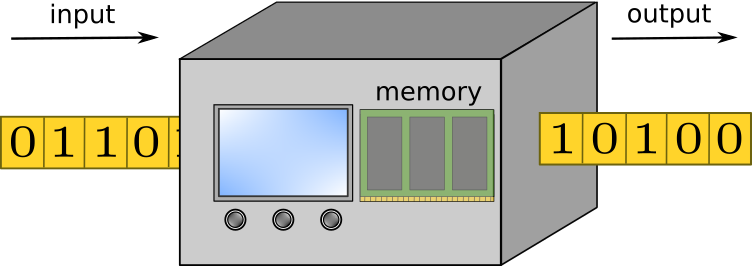
\includegraphics[width=0.7\textwidth]{images/transducer.png}
    \caption{A classical device simulating the ideal reference statistics of some KS-type experiment, consisting of sequential measurements. The device is fed a sequence of inputs (measurement choices) and produces outputs (measurement outcomes), based on its internal state prior to an input. The internal state of the device, which one can equate with a memory, stores relevant historical information about the past input-output process, on the basis of which the device generates the correct input-output statistics. After one input-output cycle, the device can update its memory state.}
    \label{fig:transducer}
\end{figure}

\begin{definition}[\cite{Barnett2015}]
An \emph{information transducer} is a tuple $(\mathcal{X},\mathcal{Y},\mathcal{S},\mathcal{T})$ where
\begin{itemize}
    \item $\mathcal{X}$, $\mathcal{Y}$ are the transducer's (finite) input and output alphabets,
    \item $\mathcal{S}$ is a (finite or countably infinite) set of internal memory states, and
    \item $\mathcal{T}\equiv\{p(S_{i+1}=s', Y_i=y\vert S_i = s, X_i=x)\}_{x,\thinspace y,\thinspace s,\thinspace s'}$ is the set of conditional ouput-transition probabilities.
\end{itemize}
More concretely, $p(S_{i+1}=s', Y_i=y\vert S_i = s, X_i=x)$ denotes the probability of the transducer outputting $y$ and transitioning to the internal state $s'$ after the $ith$ input-output cycle, conditioned on the input $x$ and internal state $s$.
\end{definition}

We require a valid classical model to produce statistics that are consistent with the infinite family of stochastic processes describing the quantum probabilities of the ideal reference experiment: $\{P(\oset{\leftrightarrow}{Y}|\oset{\leftrightarrow}{x})\}_{\oset{\leftrightarrow}{x}}$\thinspace, $\oset{\leftrightarrow}{x}$ being an instantiation of the input sequence $\oset{\leftrightarrow}{X}$.

Input-output transducers have been extensively studied within the field of computational mechanics. Of interest to us are memory-optimal classical models that produce the correct statistics $\{P(\oset{\leftrightarrow}{Y}|\oset{\leftrightarrow}{x})\}_{\oset{\leftrightarrow}{x}}$\thinspace. A transducer is memory-optimal if it stores the minimal amount of information about the past (in terms of number of bits) to make statistically correct future predictions. It has been shown that for stationary input-output processes there exists a unique memory-optimal transducer producing the correct statistics: the process' $\epsilon$-transducer \cite{Barnett2015}. The memory-optimal transducer does not store all information about the past $\oset{\leftarrow}{Z}$, as this may be highly redundant. In particular, the memory-optimal transducer does not differentiate between pasts that predict statistically identical futures. As such, the internal states of an $\epsilon$-transducer are given by the causal states of the process. 

\begin{definition}
Let $\oset{\leftarrow}{X}$, $\oset{\rightarrow}{X}$ denote the past and future stochastic input processes, respectively.
The \emph{causal states} $[\oset{\leftarrow}{z}]$ of an input-output process $\oset{\leftrightarrow}{Y}|\oset{\leftrightarrow}{X}$ are the equivalence classes on the set of pasts $\oset{\leftarrow}{z}$ with respect to the equivalence relation
\begin{equation*}
\oset{\leftarrow}{z}\;\sim_\epsilon\;\oset{\leftarrow}{z}'\;\mathrel{\vcentcolon\Leftrightarrow} \;P(\oset{\rightarrow}{Y}|\oset{\rightarrow}{X},\oset{\leftarrow}{Z}=\oset{\leftarrow}{z})= P(\oset{\rightarrow}{Y}|\oset{\rightarrow}{X},\oset{\leftarrow}{Z}=\oset{\leftarrow}{z}').
\end{equation*}
\end{definition}

\subsection{Memory-optimal classical simulation of quantum correlations}
In \cite{Cabello2018} it is shown that, for a ``causally complete" KS contextuality reference experiment, the causal states of the process' $\epsilon$-transducer correspond one-to-one to the possible quantum states $\{\ket{\Phi_{\oset{\leftarrow}{z}}}\}_{\oset{\leftarrow}{z}}$ the system can occupy after all past measurements $\oset{\leftarrow}{x}$. The assumption of causal completeness holds for many KS contextuality scenarios and in the following we will examine the odd $n$-cycle KS contextuality scenarios, in particular the KCBS scenario for $\text{n}=5$. In \cite{Cabello2018} the same analysis is performed for the Peres-Mermin (see Section \ref{sec:4dim}) and Yu-Oh (see Section \ref{sec:kcbs}) sets of measurements.

For all ideal odd $n$-cycle reference experiments, the number of possible post-measurement states tends to infinity when we increase the number of measurements in our sequence. However, the post-measurement states are not all equally probable. Figure \ref{fig:causalstates} illustrates this behaviour for the KCBS scenario $\text{n}=5$.

\begin{figure}
        %\centering
        \begin{subfigure}{0.5\textwidth}
            \centering
            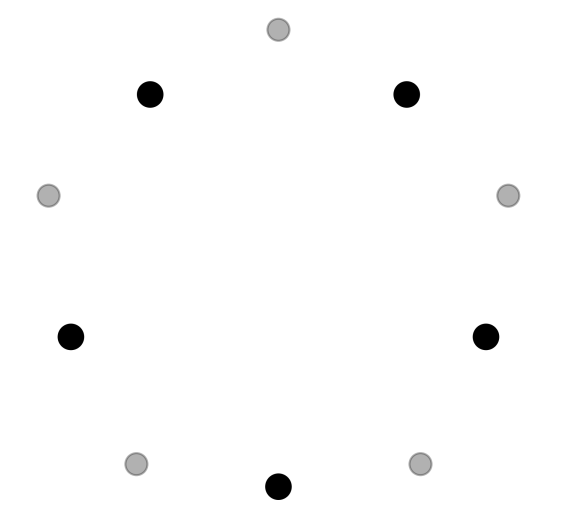
\includegraphics[width=0.8\textwidth]{images/n=5,mnts=1.png}
            \caption{one measurement}
        \end{subfigure}
        \hfill
        \begin{subfigure}{0.5\textwidth}
            \centering 
            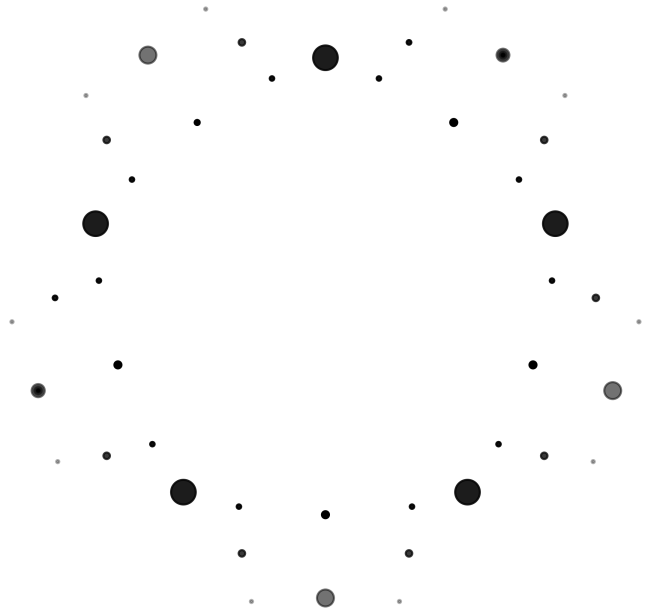
\includegraphics[width=0.8\textwidth]{images/n=5,mnts=3.png}
            \caption{three measurements}
        \end{subfigure}
        \vskip\baselineskip
        \begin{subfigure}{0.5\textwidth}
            \centering 
            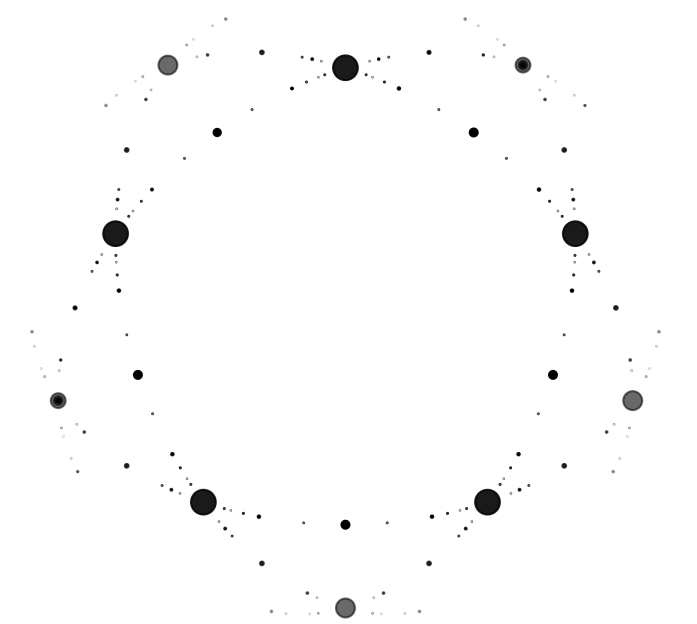
\includegraphics[width=0.8\textwidth]{images/n=5,mnts=5.png}
            \caption{five measurements}
        \end{subfigure}
        \hfill
        \begin{subfigure}{0.5\textwidth}
            \centering 
            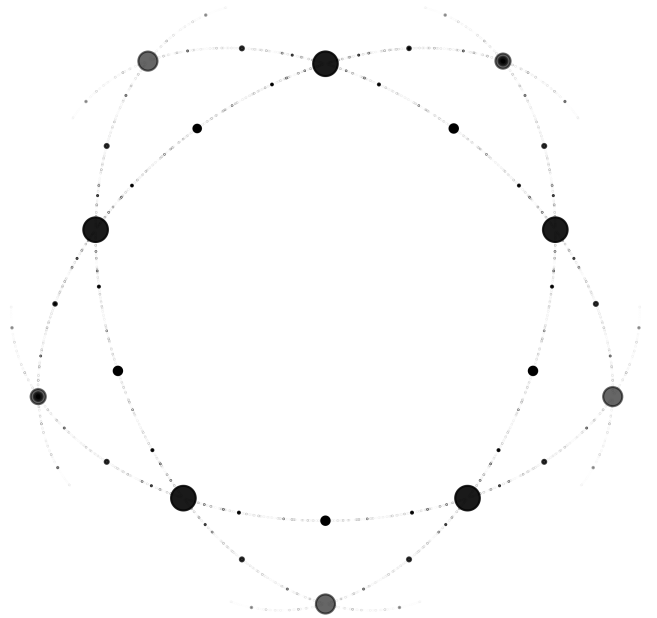
\includegraphics[width=0.8\textwidth]{images/n=5,mnts=10.png}
            \caption{ten measurements}
        \end{subfigure}
        \caption{Possible post-measurement quantum states after one, three, five, and ten measurements for the ideal KCBS experiment. The components of the post-measurement quantum states w.r.t.\ the standard qutrit basis are all real. The phases (signs) of the real qutrit states are chosen such that the corresponding vectors lie on a joint semisphere of $\mathbb{R}^3$. What is plotted are centered views of the three-dimensional plots along the negative x direction. As can be seen, the number of possible post-measurement states increases with the number of sequential measurements. The volume of a scattered point is proportional to the probability of the system being in that state after the measurements. The probability distribution over possible post-measurement quantum states becomes approximately stationary for large measurement sequences. The fact that all states lie on one of five semi-circles is a consequence of the compatibility structure of the five KCBS measurements. Analogous plots are obtained in \cite{Cabello2018} for the Peres Mermin and Yu-Oh KS contextuality scenarios.}
        \label{fig:causalstates}
    \end{figure}

Problematically, the process describing the ideal quantum experiment is not stationary, i.e.\ not invariant under translations in time, as can be seen from Figure \ref{fig:causalstates}. However, if we ``truncate" the process and consider only input-output cycles after sufficiently many initial measurements, the probability distribution over quantum states and by extension the stochastic process describing the experiment becomes stationary for all practical purposes. We only have a notion of the memory-optimal statistics-emulating classical model for the case of stationary processes. For this reason we will always consider the truncated input-output process.

To numerically compute the memory cost, we consider all possible measurement sequences of a given length k. The statistical complexity of the process (RAM memory cost) is then the Shannon entropy $H=-\sum_ip_i\log_2p_i$ of the probability distribution over all achievable post-measurement quantum states after $k$ measurements, in the limit of $k\rightarrow\infty$ \cite{Cabello2018,Barnett2015}. Recall that this probability distribution becomes approximately stationary, reflected by the above expression converging. We find the number of bits (RAM) needed by a memory-optimal simulation of the ideal reference KCBS experiment to be just over 4. The statistical complexity thus exceeds the information carrying capacity $\mathcal{C}=\log_2(3)$ of the reference qutrit. In \cite{Cabello2018} the same qualitative behaviour is observed for the Peres-Mermin and Yu-Oh sets of measurements, both of which exhibit state-independent KS contextuality. 

An interesting feature we observe is that the memory cost of simulating the ideal reference experiment for odd $n$-cycle contextuality scenarios with $\text{n}\geq5$ odd increases with the cycle length $n$, as is shown in Figure \ref{fig:ncycleRAM}. However, this increase is only logarithmic. Furthermore, what does not change is the fact that, no matter the cycle length, we need to assume an upper bound on the unknown device's information carrying capacity in order to conclude quantumness. Additionally, we need to assume that each measurement device is used only once, requiring a potentially infinite supply, as otherwise the measurement device, and not the system whose information carrying capacity we bound, could retain memory about the past stochastic process.

\begin{figure}
        \centering
        \begin{subfigure}{\textwidth}
            \centering
            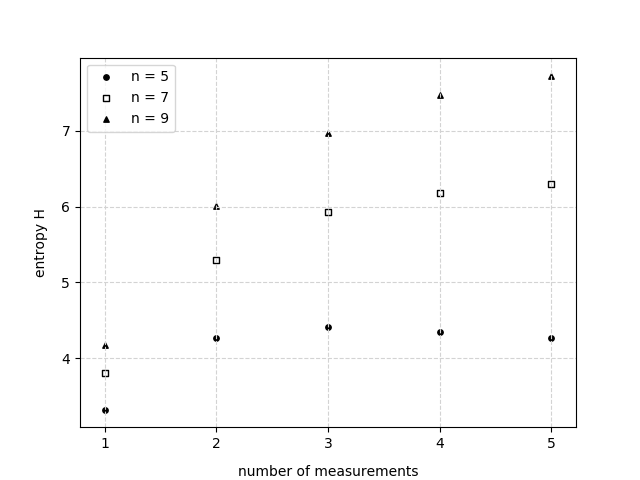
\includegraphics[width=0.7\textwidth]{images/allentropies.png}
            \caption{Plotted is the Shannon entropy of the probability distribution over all achievable post-measurement quantum states after a given number of measurements for the 5, 7, and 9-cycle KS contextuality scenarios. The probability distribution over possible post-measurement quantum states becomes approximately stationary for a sufficiently large number of measurements and the entropies thus saturate. This stationary limit of $H$ is the process' RAM memory cost, and it increases with an increasing cycle length}
        \end{subfigure}
        \vskip\baselineskip
        \begin{subfigure}{\textwidth}
            \centering 
            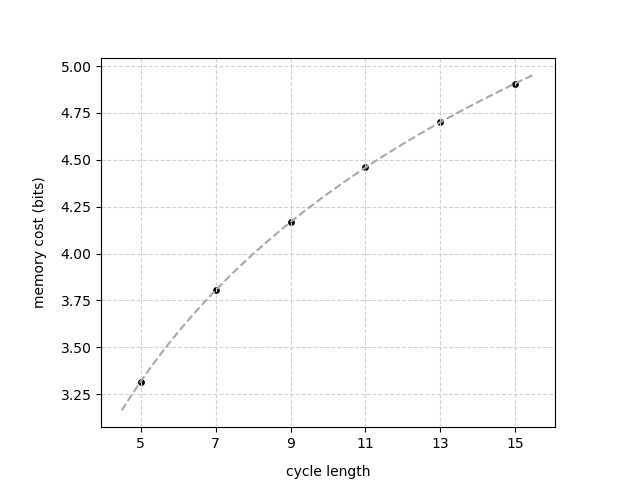
\includegraphics[width=0.7\textwidth]{images/memorycost.png}
            \caption{The RAM memory cost of classically simulating the ideal reference experiment for $n$-cycle KS contextuality scenarios increases logarithmically with the number of ideal measurements obeying cyclic compatibility that have to be implemented.}
        \end{subfigure}
        \caption{The RAM memory cost of classically simulating the ideal reference experiment for odd $n$-cycle KS contextuality scenarios in terms of the cycle length $n$.}
        \label{fig:ncycleRAM}
\end{figure}

Note that in Figure \ref{fig:ncycleRAM} only the asymptotic values of $H$ are physically relevant, characterizing the stationary regime. We have in fact adapted the protocol in \cite{Bharti2019}, by allowing the verifier to choose between $n$ measurements for every input. In particular, the verifier is not limited to just two sequential measurements within one context $i,i\oplus 1$, but can perform any measurement sequence in $\{1,\dots,n\}^m$, where $m$ is the length of the sequence. This comes with an increased measurement complexity, and the verifier must check for compatibility with the ideal reference experiment for $n^m$ measurement sequences, by comparing $n^m(2^m-1)$ correlations to the expected statistics. The measurement sequences have to be sufficiently long to approximate the stationary regime. In fact, for just two sequential measurements $i,i\oplus 1$, as proposed in \cite{Bharti2019}, one can find a classical model that reproduces the correlations of the ideal reference experiment, and requires less than one bit of memory. An information transducer with these properties is given in Figure \ref{fig:twomnts}. As such, the simulable bound on the information carrying capacity no longer exceeds the information carrying capacity of a qutrit. This highlights the need for an increased measurement complexity.

\begin{figure}
\centering
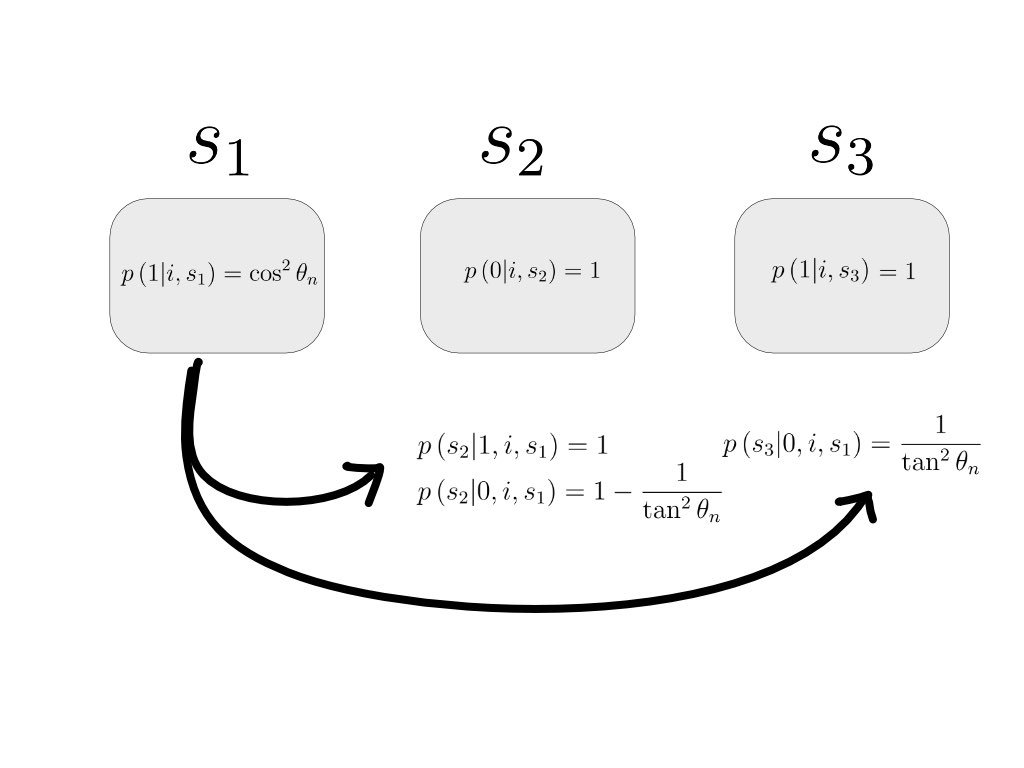
\includegraphics[width=0.8\textwidth]{images/twomnts.jpg}
\caption{Simple classical information transducer with three internal memory states, $s_1, s_2, s_3$, which reproduces all correlations of the ideal odd $n$-cycle experiment, provided that the experimenter performs only two sequential measurements $i, i\oplus 1$. The rectangles with grey border give the outcome probabilities, conditioned on the respective memory state $s_j$ and measurement $i$. The arrows indicate transitions in the internal state, and are labeled by the respective conditional transition probabilities. Prior to each input-output cycle $i,i\oplus 1$, the transducer's memory is reset to the state $s_1$.
The memory cost of this simulation, i.e. the maximal uncertainty in the internal memory state of the machine, is less than one bit (after one measurement, the system is in one of two states with unequal probability), and in particular does not exceed the qutrit information carrying capacity. This simple example is meant to motivate an increased measurement complexity, in order to establish a clear separation in terms of resources between the ideal qutrit and any classical simulation.}
\label{fig:twomnts}
\end{figure}





\chapter[A revised notion of non-classicality \\ Spekkens contextuality]{A revised notion of non-classicality \\ \huge{Spekkens contextuality}}
\lhead{\emph{Spekkens contextuality}}
\label{sec:spekkcont}
\section{Outcome determinism for unsharp measurements (ODUM)}
\label{sec:odum}
We want a notion of classicality that accomodates unsharp measurements and is robust to noise. A first approach might entail simply extending KS non-contextuality to general POVM measurements, in the sense that a classical HVM description assigns a conditional probability  $p\in\{0,1\}$ to all positive semi-definite operators, such that for every resolution of the identity only one operator receives the valuation $1$. This incremental approach has been given the name ``ODUM", which stands for ``outcome determinism for unsharp measurements". The problem with ODUM is that it runs into numerous inconsistencies, as convincingly argued in \cite{Spekkens2014}. We confine ourselves to the most immediate inconsistency: Consider the quantum experiment consisting of an experimenter repeatedly performing the trivial POVM $\{\frac{\mathbb{1}}{2},\frac{\mathbb{1}}{2}\}$ on some arbitrary preparation $\rho$. Any classical value assignment to positive semi-definite operators in accordance with ODUM is in conflict with the normalization conditions for general ontological models in Section \ref{sec:hvm}. In particular, for a given ontic state $\lambda$, either the added probabilities of the two outcomes is zero or exceeds one. Thus, either this trivial POVM is non-classical according to the extended notion just presented, or the new notion is not meaningful. The trivial POVM corresponds to a fair coin flip - it can be implemented by simply throwing away the system and generating a random bit. Such a ``measurement" should by all means be considered classical. For this implementation, the only sensible choice is to assign to every every ontic state $\lambda$ the conditional probability $\frac{1}{2}$, as measurement and system are completely decoupled. The same line of reasoning leads to the conclusion that the approach in Section \ref{sec:cswhierarch} cannot be extended to general unsharp measurements, as this produces inconsistencies when treating QM.

\section{Operational approach due to Spekkens}
\label{sec:spekkensopappr}
The previous examples highlight the need for a new notion of contextuality that captures the spirit of KS non-contextuality, but is applicable to realistic experimental scenarios. Let us take a step back and identify common features of the contextuality scenarios discussed so far, which led to behaviour we deemed non-classical. The setting was in all cases for the most part identical: we considered sets of projective measurements, with the key property that a given projector was shared amongst multiple measurements. Identical projectors appearing in multiple measurement contexts were crucial for proving a contradiction. Spekkens' approach captures this key feature and operationalizes the underlying assumptions. In QM, a positive semi-definite operator defines an operational equivalence class, in the sense that measurement events which are operationally indistinguishable for all state preparations must be represented by the same operator. An analogous observation applies to density operators describing the preparation of a system.
On that account, instead of assuming a projector to be part of several measurement contexts, Spekkens assumes certain measurement events to be operationally equivalent; we will formalize this shortly. Assuming KS non-contextuality, the implication of a projector appearing as part of multiple measurements is that it must be assigned the same conditional probability $\{0,1\}$ by the ontological model, for all ontic states $\lambda$. In other words, operationally equivalence implies an identical ontological representation. We will find that Spekkens' revised notion of non-contextuality follows exactly this prescription.  

In \cite{Spekkens2005}, Spekkens introduces a largely operational notion of contextuality for preparations, measurements, and transformations. It is a revision of KS contextuality that addresses several shortcomings of the traditional definition. Contextuality is generalized to apply to arbitrary operational theories. In comparison, KS contextuality is limited to the scope of QM, as it is defined within the framework of quantum theory. Furthermore, the revised definiton will not assume outcome determinism at an ontic level, accomodating HVM whose indicator functions are more general mappings $\Lambda\mapsto [0,1]$. Taking QM as operational theory, Spekkens contextuality extends to arbitrary measurements, including physical, non-projective ones. In fact, within the Spekkens framework, measurements, preparations, and transformations can be considered black box devices, i.e.\ primitives of which one can compose an experiment. An operational theory makes predictions about these operational primitives, i.e.\ assigns probabilities to measurement outcomes that are consistent with experimental observations. In QM, for instance, outcome probabilities are given by the Born rule, where we posit that every preparation is operationally fully specified by a density operator and every measurement by a POVM. A Spekkens non-contextual operational theory is one that is compatible with a Spekkens non-contextual ontological model, which we will define shortly. Spekkens' revised concept of non-contextuality will serve as a new, more suitable notion of classicality that is in particular compatible with unsharp measurements.

This section only discusses Spekkens non-contextuality for preparations and measurements, as transformations will not be relevant to our discussion\footnote{Consider a prepare-and-measure type experiment that consists of an initial state preparation, followed by some transformation of the system, and finally a measurement. We may consider the transformation as part of the initial preparation procedure, or as part of the final measurement, and describe the experiment solely in terms of preparation procedures and measurements.}. Preparations and measurements will be represented as outlined in Section \ref{sec:hvm}. In the following, if not stated otherwise, the term ``contextuality" and all variant forms will refer to Spekkens contextuality.

The essence of what it means for an ontological model to be non-contextual can be summarized as follows:
An ontological model of an operational theory is \emph{non-contextual} if the operational equivalence of two experimental procedures, i.e.\ two preparations or two measurements, 
implies that they have an equivalent representation in the ontological model.
Two experimental procedures are operationally equivalent if they cannot be distinguished by any measurement statistics. 

Let us formalize the above, starting with preparation non-contextuality. We can define an equivalence relation on the set of all preparation procedures $P$ that partions the set into operational equivalence classes $[P]$. By the guiding principle above, we require equivalent preparations to have the same ontological representation in a non-contextual HVM.

\begin{definition}[\cite{Spekkens2005}]\hfill\break
\label{def:prepnc}
Two preparation procedures $P,P'$ are \emph{equivalent}, denoted $P\sim P'$, if 
\begin{equation*}
    \forall \text{ measurements } M,\thinspace \forall \text{ measurement outcomes } k\thinspace:\thinspace p(k\vert P,M)=p(k\vert P',M)\thinspace.
\end{equation*}

An ontological model is \emph{preparation non-contextual} if equivalent preparations have identical associated probability density functions on the ontic state space: 
\begin{equation*}
    \forall \text{ preparations } P\thinspace:\thinspace \mu_{P}=\mu_{[P]}\thinspace.
\end{equation*}
\end{definition}

Measurement non-contextuality is defined in an analogous manner:

\begin{definition}[\cite{Spekkens2005}]\hfill\break
\label{def:mntnc}
Two measurement procedures $M,M'$ are \emph{equivalent}, denoted $M\sim M'$, if their outcomes can be associated one-to-one and 
\begin{equation*}
    \forall \text{ outcomes } k\thinspace,\thinspace \forall \text{ preparations } P\thinspace:\thinspace p(k\vert P,M)=p(k\vert P,M')\thinspace.
\end{equation*}

An ontological model is \emph{measurement non-contextual} if equivalent measurements have identical associated indicator functions: 
\begin{equation*}
    \forall \text{ measurements } M\thinspace,\thinspace \forall \text{ outcomes } k\thinspace:\thinspace \xi_{M,k}=\xi_{[M],k}\thinspace.
\end{equation*}
\end{definition}

Spekkens proves three no-go theorems for ontological models of QM \cite{Spekkens2005}. These rule out preparation non-contextual, measurement non-contextual, and transformation non-contextual models, respectively. All three proofs apply to two-dimensional Hilbert spaces, making them stronger than traditional proofs of contextuality.

Whenever referring to a non-contextual ontological model, without specifying preparation or measurement contextual, we  will assume the ontological model to be both preparation and measurement non-contextual. As the reasons for assuming classical correlations to be compatible with a measurement non-contextual HVM description are the same as those for preparation non-contextuality, the combination of both is the only natural assumption of non-contextuality.

We now discuss to what extent non-contextuality is a sensible notion of classicality. A contextual ontological model implies a difference in reality that cannot be observed. Such a model is in conflict with Leibniz' ``Identity of Indiscernibles" \cite{Buchanan2019,Spekkens2019}. Leibniz's principle states that two empirically indistinguishable scenarios are to be ontologically equivalent. As such, it rejects ontological models for which there exist ontologically distinct, but empirically indistinguishable scenarios. Recall that, within QM, KS non-contextuality can be seen as a generalization of Bell's notion of local determinism to non-remote measurement contexts. One can also link Leibniz' principle, which is at the heart of Spekkens' revised notion of contextuality to Bell's notion of local causality. Like before, local causality is the weaker assumption, which is owed to the fact that Bell-type experiments impose additional constraints on the experiment's causal structure:

In principle, it might well be the case that an agent's free choice of measurement can have a causal influence on a remote system and alter the ontic or "matter of fact" state of that system. However, physicists have yet to devise an experiment producing correlations that are in conflict with the no-signalling principle, which is reinforced by special relativity. Therefore, to the best of our knowledge, such causal influence, if it exists, is not detectable. This in turn means that an agent in the remote frame of reference can detect no difference in the physical properties of his system for different free choices of measurement. Local causality is the assumption that there is in fact no difference at the ontic level, and thus provides the most natural explanation for our inability to detect a causal influence. Another, more hair-raising explanation could be that all possible ensemble preparations accessible to an experimenter are too spread out to resolve minor differences in the conditional probabilities. The assumption of local causality just corresponds to Leibniz' principle applied to Bell-type experiments with space-like separated measurements. The assumption of Spekkens non-contextuality simply extends the applicability of Leibniz's principle to arbitrary prepare-and-measure type experiments, in particular those without remote subsystems.

Just as local causality is motivated by the no-signalling principle, local causality providing the most natural explanation for our apparent inability to communicate superluminally, a point can be made that non-contextuality is perhaps equally well motivated by Leibniz' Identity of indiscernibles. Analogously to local causality, non-contextuality is the most natural explanation for operational equivalences. Spekkens points out that the credentials of Leibniz' principle parallel those of no-signalling and that it was critical in Einstein's conception of relativity \cite{Buchanan2019,Spekkens2019}. Take for instance the equivalence principle which states that one cannot distinguish between being at rest in a uniform gravitational field and accelerating uniformly through free space. Within Newtonian mechanics the two scenarios are ontologically distinct, as one's absolute acceleration differs in both cases. On his way to general relativity, Einstein reasoned that the empirical indistinguishablitiy of both scenarios implies that they should be treated as ontologically equivalent by a physical theory, a powerful invocation of Leibniz's principle that reshaped our perception of reality. An almost identical line of reasoning is found in Einstein’s 1905 paper ``On the electrodynamics of moving bodies" \cite{Einstein1905}. He notes that the predictions of Maxwell's equations depend only on relative motion. For example, the current induced in a coil will have the same magnitude and direction, no matter if we consider a magnet to be moving through the coil or the coil moving through the field of the magnet with equal but opposite velocity. To Einstein, this empirical indistinguishability was in conflict with the prevailing aether theories of the time. An aether would define a distinguished frame of reference, rendering the two empirically equivalent induction experiments ontologically distinct. Once again, Einstein's invocation of Lebniz' principle lead him to abandon aether theory and conceive relativity theory, in which both scenarios are equivalent.

One can lift KS non-contextuality inequalities to Spekkens non-contextuality inequalities by substituting assumptions about operator compatibility and sharpness for assumptions about operational equivalences \cite{Kunjwal2019}. Like before, these lifted non-contextuality inequalities, when violated, bear witness to the quantumness of the system, in the Spekkens sense. Violations of non-contextuality inequalities that prove nature's incompatibility with a non-contextual HVM description have been observed in experiments involving photonic qubit systems \cite{Mazurek2016}. While the lifted non-contextuality inequalities no longer make unphysical assumptions about the measurements themselves, they introduce two new practical complications: the issue of tomographic completeness, and that of exact operational equivalence. Experimental tests of non-contextuality inequalities assume that we can implement a tomographically complete (TC) set of measurements, relative to the accessible\footnote{An ``accessible" preparation procedure is one that is implemented by the experimental apparatus at hand, and whose statistics are recorded as part of the experiment.} preparations, and a TC set of preparations, relative to the accessible measurements. The reason for this is that, according to Definitons \ref{def:prepnc}, \ref{def:mntnc}, two experimental procedures can only be asserted operationally equivalent if the two procedures are operationally indistinguishable, for all possible prepare-and-measure-type experiment that utilize them. For instance, two preparations are only operationally equivalent if they produce the same statistics for all possible measurements, requiring in principle an infinite number of tests. In practice, we aim to identify a TC set of measurements with respect to the two preparations, as defined in REF, such that there is a functional relationship between the statistics of an arbitrary measurement performed on one of the available preparations and the statistics of only the measurements of the TC set. As such, if two preparations are operationally equivalent with respect to a TC set of measurements, they are operationally equivalent with respect to all measurements. Within QM, a TC set of measurements for a qubit system is given by the three Pauli measurements $\sigma_x$, $\sigma_y$, and $\sigma_z$, that together determine the three Bloch vector components of an arbitrary state.

\begin{definition}[\cite{Pusey2019a}]
\label{def:tc}
A set of binary measurements (with outcomes 0,1) $\mathcal{M}_C$ is tomographically complete (TC), relative to a set of preparations $\mathcal{P}$, if for any measurements $M$ (not necessarily contained in $\mathcal{M}$) with outcome set $\mathcal{K}_{M}$ there exists a deterministic function $f_M:\mathcal{K}_{M}\times[0,1]^{\vert\mathcal{M}_C \vert}\rightarrow [0,1]$ with the properties that
\begin{enumerate}
\item $\forall k\in\mathcal{K}_{M}:\;$ $f(k\,,\,\cdot):[0,1]^{\vert\mathcal{M}_C\vert}\rightarrow [0,1]$ is a linear mapping, and
\item $\forall k\in\mathcal{K}_{M}\,\forall P\in\mathcal{P}$: $p(k\,\vert\, P,M)=f_M(k,\{p(0\,\vert\,P,M')\}_{M'\in\mathcal{M}_C})$,
\end{enumerate}
where $p(k\,\vert\, P,M)$ is the empirical probability of obtaining the outcome $k$ when performing the measurement $M$ on a system prepared like $P$.
\end{definition}
Note that Condition 1 ensures that the mapping $f_M$ is compatible with convex mixtures of preparation procedures.

Problematically, without additional assumptions, we can in practice never declare a set of measurements to be TC with respect to some set of preparations. What we can do is try our best to refute such a claim. Additionally, there are tests of contextuality that account for some number of unknown degrees of freedom, in particular some number of unknown measurements that complete the accessible measurements to a TC set \cite{Pusey2019a}. These strengthened tests of contextuality require knowledge about an upper bound on the information carrying capacity of the system, i.e. the amount of information (in bits) that one can encode in the state of the system in a retrievable manner. By implementing more preparations and measurements one can in principle account for an arbitrary number of unknown degrees of freedom, although the trade-off is exponential. Section \ref{sec:protocols} will make use of the results in \cite{Pusey2019a}, which will ultimately allow us to certify the quantumness of the unknown device in a robust manner, assuming an upper bound on its information carrying capacity. Just like in the case of KS contextuality, where one had to assume operator compatibility and sharp measurements, we cannot expect to devise a fully device-independent self-testing protocol based on non-contextuality.

Another issue with experimental tests of contextuality is that Definitions \ref{def:prepnc}, \ref{def:mntnc} assume exact operational equivalences, requiring infinite precision. This problem has been tackled in \cite{Pusey2018,Mazurek2016}. Let us for the moment consider operational equivalences amongst preparations. The key is noticing that performing measurements on some set of preparations defines the statistics for all preparations in the convex hull. As part of post-processing, we can define new preparations in the convex hull, whose statistics we know, and that are exactly operationally equivalent. The price to pay is that these new preparations may be less optimal than the original ones. This ``fitting" process that establishes exact operational equivalences is done within the framework of generalized probabilistic theories (GPT). Operational equivalences amongst measurements are treated in an analogous manner. The protocol we propose in Section \ref{sec:protocols} in fact only assumes approximate operational equivalence of certain preparations.

Finally, we wish to understand how KS contextuality and Spekkens contextuality are related. It turns out that a Spekkens non-contextual ontological model of QM assign deterministic outcomes to projective quantum measurements and induces a KS non-contextual outcome assignment, like in Definition \ref{def:kscontherm}.
KS non-contextuality is an assumption that restricts the ontological representation of compatible (commuting) projective measurements. Let us therefore examine what conditions Spekkens non-contextuality imposes on the ontological representation of compatible measurements. Spekkens non-contextuality covers arbitrary, not necessarily sharp, measurements and is applicable to arbitrary operational theories. Therefore, recall Definition \ref{def:compat}, which defines what it means for two measurements to be compatible, purely in operational terms.

Let $M_{1}$ and $M_{2}$ be compatible measurements according to Definition \ref{def:compat}, and $M_{12}$ a dual outcome measurement that jointly realizes $M_1$ and $M_2$. By definition, the measurement procedure $M_{1}$ is operationally equivalent to measuring $M_{12}$ and discarding register two. Analogously, the measurement procedure $M_{2}$ is operationally equivalent to measuring $M_{12}$ and discarding register one. What can be said about the ontological representation of compatible measurements within a Spekkens non-contextual model? In a Spekkens non-contextual ontological model, operationally equivalent measurement procedures have identical associated indicator functions. For the measurements $M_{1}$, $M_{2}$, and $M_{12}$ like above, this implies:
\begin{align*}
\forall\thinspace\lambda\in\Lambda,\thinspace\forall \thinspace P,\thinspace\forall\thinspace a_{k}:p(a_{k}\thinspace\vert\thinspace M_{1},P,\lambda)=\sum_{b_{j}}p(a_{k},b_{j}\thinspace\vert\thinspace M_{12},P,\lambda)\\
\forall\thinspace\lambda\in\Lambda,\forall\thinspace P,\thinspace\forall\thinspace b_{k}:p(b_{k}\thinspace\vert\thinspace M_{2},P,\lambda)=\sum_{a_{i}}p(a_{i},b_{k}\thinspace\vert\thinspace M_{12},P,\lambda)
\end{align*}
Consequently, a Spekkens measurement non-contextual ontological model is one for which the probability of measuring say $M_{1}$ and obtaining the outcome $a_{k}$, conditioned on the system being in any ontic state, is independent of what other compatible measurements are simultaneously performed. If we consider QM as operational theory, this is the essence of KS non-contextuality, as discussed in Section \ref{sec:kscont}, with the notable difference that we have decoupled outcome determinism from context independence.

Interestingly, it can proven that a Spekkens non-contextual ontological model must fix the outcomes of sharp measurements deterministically \cite{Spekkens2014}. This result is robust, in the sense that ``almost sharp" measurements are assigned outcomes ``almost deterministically". Thus, for projective measurements, the notion of Spekkens non-contextuality reduces to KS non-contextuality. For Spekkens non-contextual ontological models, outcome determinism for sharp measurements can thus be derived from within the framework itself, and is not an assumption introduced ad-hoc, as was the case for KS non-contextuality.
\chapter{Protocol based on Spekkens contextuality}
\lhead{\emph{Protocol based on Spekkens contextuality}}
\label{sec:protocols}
We now generalize the self-testing result in \cite{Bharti2019}, which was discussed in Section \ref{sec:contselftesting}, to the framework of Spekkens contextuality. In particular, this will lift the usual restriction to noise-free projective measurements. Additional features will be discussed in Section \ref{sec:discussion}. The protocol we will consider assumes approximate operational equivalences for some preparations, as well as an upper bound on the unknown system's information carrying capacity, much like the protocol in Section \ref{sec:contselftesting}.

Let $n\geq 5$ be an odd integer. The protocol we consider is again reminiscent of the ideal $n$-cycle reference experiment \ref{eqn:ncycleideal}. As such, we assume an experimenter to be able to freely choose between $n$ three-outcome measurements $\{M_i\}_{i=1}^n$ with outcomes $m_1$, $m_2$, $m_3$. We assume measurements to be chosen according to a uniform distribution and denote measurement events by  $m_k\thinspace\vert\thinspace M_i$, or $m_k,m_l\thinspace\vert\thinspace M_i,M_j$ for two sequential measurements. As shown in Figure \ref{fig:ncycleselftesting}, for ideally operating devices, the measurement events $m_1 \thinspace\vert\thinspace M_i$ correspond to the rank-one projectors $\vert u_i^{(n)}\rangle\langle u_i^{(n)}\vert$ defined by \ref{eqn:ncycleideal}. Further, in the ideal case, the measurement events \begin{equation*}
m_3\thinspace\vert\thinspace M_i\equiv m_1\thinspace\vert\thinspace M_{i\oplus 1}\equiv\vert u_{i\oplus 1}^{(n)}\rangle\langle u_{i\oplus 1}^{(n)}\vert
\end{equation*}and the events $m_2\thinspace\vert\thinspace M_i$ correspond to the projectors 
\begin{equation*}
m_2\,\vert\,M_i\equiv \mathbb{1}-\vert u_i^{(n)}\rangle\langle u_i^{(n)}\vert-\vert u_{i\oplus 1}^{(n)}\rangle\langle u_{i\oplus 1}^{(n)}\vert
\end{equation*} onto the pure qutrit state completing the orthogonal triad $\subset \mathbb{C}^3$. In Figure \ref{fig:ncycleselftesting}, the events $m_3\thinspace \vert\thinspace M_i$ and $m_1\thinspace\vert\thinspace M_{i\oplus 1}$ are ``non-overlapping", despite corresponding to the same ideal projectors, to highlight that we do not need to assume operational equivalence, contrary to the assumptions made in \cite{Kunjwal2019}.

\begin{figure}
	\begin{subfigure}[t]{0.45\textwidth}
    	\centering
    	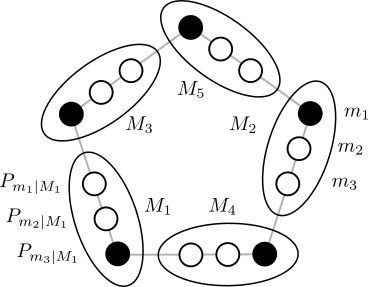
\includegraphics[width=\textwidth]{images/mntsandpreps.png}
        \caption{}
	\end{subfigure}
	\hfill
    \begin{subfigure}[t]{0.45\textwidth}
    	\centering 
        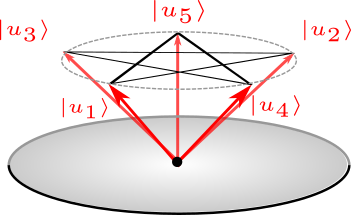
\includegraphics[width=0.8\textwidth]{images/kcbsrefstates.png}
        \caption{}
    \end{subfigure}
    \caption[]{\textbf{(a):} Measurement events and retrospective preparations corresponding to a self-testing scenario consistent with cycle length $n=5$. The experimenter can choose from five three-outcome measurements $M_i$, with outcomes $\{m_1,m_2,m_3\}$. In post-processing, the experimenter defines $2n$ preparations 

\begin{minipage}{\linewidth}
\vspace{0.2em}
     \begin{equation*}
        \{P_{m_k\vert M_i}\}_{k,i}\hspace{1em}\text{, for } k\in\{ 1,2\}\text{ and }i\in\{ 1,\dots,n\}.
     \end{equation*}    
\end{minipage}

\vspace*{0.7em} 
We define $P_{m_3\vert M_i}\coloneqq P_{m_1\vert M_{i\oplus 1}}$. In the ideal case, the measurement events $\{m_k\vert M_i\}_{k\in\{1,2,3\}}$ correspond to rank-one projectors onto the orthogonal triad $\subset \mathbb{C}^3$ containing the cycle states $\vert u_i\rangle$ and $\vert u_{i\oplus 1}\rangle$. Furthermore, in the ideal case, the preparations $P_{m_k\vert M_i}$ are pure states that coincide with the vectors in this triad. The measurement events $m_3\vert M_i$ and $m_1\vert M_{i\oplus 1}$ are non-overlapping to illustrate that the self-testing protocol does not assume operational equivalence of these, despite the fact that they correspond to the same rank-one projector onto $\vert u_{i\oplus 1}\rangle$ in the ideal case. \textbf{(b):} Juxtaposition with the cycle states belonging to the odd $n$-cycle scenario for $n=5$. Figure (a) can be seen as a top view of (b), with every black dot corresponding to a cycle state $\vert u_i\rangle$.
}
\label{fig:ncycleselftesting}
\end{figure}

Like in Section \ref{sec:contselftesting}, we assume i.i.d.\ rounds, i.e. the devices to operate in an identical manner for all rounds of the protocol, in particular independently of previous input-output cycles. This allows us to lift relative frequencies to probabilities. We will discuss all other assumptions in due time. The protocol consists of the following steps:
\begin{enumerate}
\item The experimenter prepares the system in a distinguished preparation $P_0$ by selecting the appropriate setting on the corresponding device.
\item The experimenter samples from a uniform distribution and selects two integers $(i,j)\in\{1,\dots,n\}^2$ at random.
\item The experimenter performs the measurements $M_i$, $M_j$ in sequence, first $M_i$, then $M_j$. He does so by selecting the respective settings on the corresponding devices and records the outcomes.
\item Steps 1-3 are repeated to obtain estimates for the probability distributions \\ $p((m_k,m_l)\thinspace\vert\thinspace (M_i,M_j),P_0)$. 
\item Additionally, the experimenter performs single measurements on two auxilliary preparations $P_1$ and $P_2$ he can choose from and obtains estimates for the probability distributions $p(m_k\thinspace\vert\thinspace M,i, P_j)$, for $j\in{1,2}$.
\item Post-processing
	\begin{enumerate}
	\item Certificate of quantumness
	\item Bounding compatible quantum models
	\end{enumerate}
\end{enumerate}

We write the free choice of measurements $(M_i,M_j)$ and subsequent outcomes $(m_k,m_l)$ as ordered lists to indicate that the distributions $p((m_k,m_l)\thinspace\vert\thinspace (M_i,M_j),P_0)$ are in general not independent of the order, since we do not assume any underlying compatibility relations like we did in Section \ref{sec:contselftesting}. In the ideal case, the distinguished preparation $P_0$ corresponds to the $\ket{0}$ qutrit state, which produces a maximal violation of the KCBS inequality. Additionally, we assume access to two additional auxilliary preparations, $P_1$ and $P_2$, which we require to establish approximate operational equivalences during post-processing. In the ideal case the preparations $P_1$ and $P_2$ correspond to the $\ket{1}$ and $\ket{2}$ qutrit states, forming an orthogonal triad with $\ket{0}$. The convex combination $\frac{1}{3}\sum_{i=0}^2 P_i\equiv\frac{1}{3}\sum_{i=0}^2\ket{i}\bra{i}=\frac{\mathbb{1}}{3}$ corresponds to the fully mixed state $\frac{\mathbb{1}}{3}$, as does the convex combination with equal weights of the ideal projectors corresponding to the measurement events $\{m_k\vert M_i\}_{k=1}^3$, for all $i\in\{1,\dots,n\}$. Here, we implicitly defined the convex combination of two preparations to be the preparation that is implemented by generating a random number and performing the preparation procedure associated with that outcome. We note that Steps 1-4 of the protocol correspond almost one-to-one to the steps of the protocol in \cite{Bharti2019}, which was discussed in Section \ref{sec:contselftesting}, the only difference being that the experimenter now freely chooses between $n^2$, as opposed to $n$ measurement settings.

We now elaborate on Step 6 of the protocol, detailing how an agent may post-process the acquired data, with the goal of self-testing the apparatus. The experimenter retrospectively defines $2n$ preparations, which we denote $P_{m_k\vert M_i}$, for $i\in\{1,\dots,n\}$ and $k\in\{1,2\}$. As suggested by the notation, $P_{m_k\vert M_i}$ is prepared by performing the measurement $M_i$ on a system initially prepared like $P_0$, and conditioning on the outcome $m_k$. We refer to these preparations as retrospective, since they are not directly implemented by the experimenter. However, one can infer the relevant statistics $p(m_k\thinspace\vert\thinspace M_i, P_{m_l\vert M_j})$ for these preparations from the distributions $p((m_k,m_l)\thinspace\vert\thinspace (M_i,M_j))$:
\begin{equation*}
p(m_k\thinspace\vert\thinspace M_i, P_{m_l\vert M_j})=\frac{p((m_k,m_l)\thinspace\vert\thinspace (M_i,M_j))}{\sum_{k'\in\{1,2\}} p((m_{k'},m_l)\thinspace\vert\thinspace (M_i,M_j))}.
\end{equation*}
These retrospective preparations will be used in Section \ref{sec:certifyquant}, where we introduce a criterion to certify the quantumness of the apparatus.

The experimenter can also infer the distribution $p(m_k\thinspace\vert\thinspace M_i, P_0)$ from the correlations \\$p((m_k,m_l)\thinspace\vert\thinspace(M_i,M_j),P_0)$:
\begin{equation*}
p(m_k \thinspace\vert\thinspace M_i, P_0)=\sum_{l,j}\frac{1}{n}p((m_k,m_l)\thinspace\vert\thinspace (M_i,M_j),P_0).
\end{equation*}
These will become relevant in Section \ref{sec:boundingmodels}, when bounding the compatible quantum models.
\section{Step 6a: Certificate of quantumness}
\label{sec:certifyquant}
By coarse-graining, we obtain $2n$ binary measurements from the $n$ three-outcome measurements $M_i$\,: for each $M_i$, we ``lump together" the outcomes $m_2$, $m_3$, and $m_1$, $m_3$. In total, we define $2n$ binary measurements and $2n$ preparations during post-processing. We denote the outcomes of the $2n$ binary measurements as $0$, $1$, where the outcome $0$ corresponds to the two coarse-grained measurement events. If we consider the ideal reference experiment \ref{eqn:ncycleideal}, the outcomes $0$, $1$ correspond to the eigenvalues of the rank-one projectors we can associate with each of the binary measurments. There are $n$ ideal binary measurements that probe the probability of finding the system in one of the $n$ one-dimensional subspaces spanned by the $n$ cycle states. The other $n$ ideal binary measurements correspond to rank-one projectors onto states in an orthogonal triad containing two cycle states. For the extent of this subsection we will for simplicity index the $2n$ binary measurements and preparations like $\{M_i\}_{i\in\{1,\dots,2n\}}$ and $\{P_i\}_{i\in\{1,\dots,2n\}}$. For ideal measurements and preparations, we can choose the order such that the ideal measurement $M_i$ is the rank-one projector onto the ideal pure state preparation $P_i$. Therefore, for ideal devices, the retrospective preparations and binary measurements, if ordered in this manner, satisfy \begin{equation}
\label{eqn:epsilon}
\epsilon \coloneqq \max_i p(0\vert M_i, P_i)\stackrel{\text{ideal}}{=}0.
\end{equation} 
For noisy devices, we expect to find an ordering for which \ref{eqn:epsilon} is approximately satisfied, with the parameter $\epsilon$ characterizing the amount of noise. The parameter $\epsilon$ can be determined from the observed statistics during post-processing.

Apart from the noise-characterizing parameter $\epsilon$, the other important figure of merit is
\begin{equation*}
\eta\coloneqq \min_{\substack{i,j \\ i\neq j}} p(0\vert M_i, P_j).
\end{equation*}
The parameter $\eta$ can be thought of as a measuring the maximum overlap or closeness of distinct states. Roughly speaking, the smaller $\eta$, the closer distinct states are. As such, we expect $\eta$ to decrease as the cycle length $n$ increases. 

Let $m=2^k$. In Appendix B of \cite{Pusey2019a} it is proven that for a set of preparations $\{P_i\}_{i=1}^m$ and measurements $\{M_i\}_{i=1}^m$, producing statistics obeying $\epsilon<\frac{1}{4}\eta^2$, to be compatible with a (preparation) non-contextual ontological description, requires at least $k$ binary measurements in any set that is TC with respect to the preparations $\{P_i\}_{i=1}^m$. The intuition behind this is the following: From the statistics of the $m$ preparations $\{P_i\}_{i=1}^m$ one can infer the statistics of any preparation in the convex hull of the $\{P_i\}_{i=1}^m$. If the $m$ preparations are not very ``close", as measured by $\eta$, relative to their sharpness, as measured by $\epsilon$ (this is enforced by the condition $\epsilon<\frac{1}{4}\eta^2$), then the associated probability density functions $\{\mu_i\}_{i=1}^m$ will have non-significant overlap. In particular, if we regard the $m$ probability density functions on the ontic state space $\Lambda$ as vectors $\{v_i\}_{i=1}^m$ in $\mathbb{R}^{\vert \Lambda \vert}$, then the proof in Appendix B of \cite{Pusey2019a} establishes that the $m=2^k$ vectors vary in $k$ linearly independent directions. Demanding preparation non-contextuality, every distinct preparation in the convex hull of the $\{P\}_{i=1}^n$ must produce different predictions for at least one of the measurements in a TC set. Finally, \cite{Pusey2019a} notes that the function mapping a probability density function $\mu_j$, or rather the corresponding vector in $\mathbb{R}^{\vert \Lambda \vert}$ to the probability $p(m_k\thinspace\vert\thinspace M_i,\mu_j)$ of obtaining the outcome $m_k$ when performing the measurement $M_i$ for the initial preparation $\mu_j$ is linear. Hence, such mapping $\mathbb{R}^{\vert \Lambda \vert}\rightarrow\mathbb{R}$ is of the form $(x_1,\dots,x_{\vert \Lambda \vert})\mapsto a_1 x_1+\dots + a_n x_n = \vec{a}\cdot \vec{x}$ with $0 \leq a_i \leq 1$, and $x_i$ the components w.r.t\ the standard basis of $\mathbb{R}^{\vert \Lambda \vert}$. Binary measurements can therefore only distinguish between preparations along a single direction, $\vec{a}$. Preparations whose ontological representations differ w.r.t.\ directions orthogonal to $\vec{a}$, are assigned the same probabilities by the binary measurement characterized by $\vec{a}$. A TC set of measurement must contain at least $k$ binary measurements for $k$ ``linearly independent"` preparations, if we demand compatiblity with a preparation non-contextual ontological model.

We now turn to the bounded memory assumption required by the protocol, which relies on the results of \cite{Pusey2019a}, the relevant ones of which were sketched above. Assume that the experimenter has access to $n\geq 5$ three-outcome measurement settings, like we considered at the beginning of Section \ref{sec:protocols}, where $n$ is odd (think of $n$ as the cycle-length). Further, let $k$ be the largest integer satisfying $2n\geq 2^{k+1}$. To certify quantumness, we assume that there exists a TC set of measurements, relative to the $2n$ retrospective preparations, with $k$ binary measurements, i.e. that $k$ binary measurements are sufficient to fully characterize the statistics of the accessible preparations. If we find the condition $\epsilon<\frac{1}{4}\eta^2$ to be satisfied, we consider the system to be quantum.  How does this assumption relate to the assumption of bounded memory in Section \ref{sec:memoryass}? 

In Section \ref{sec:memoryass}, we studied the minimal memory (in bits) a classical simulation requires to reproduce the ideal statistics. 
For $m\geq1$ sequential (binary) measurements, consider the $2^m$ accessible preparation procedures that consist of subjecting the system to $m$ binary measurements and conditioning on one of the $2^m$ outcome strings. Some of these preparations can be identified, as they are operationally indistinguishable and result in the same causal state. To ensure correct operation, an optimal classical device retains minimal information about the past input-output process, and retrieves that information when confronted with a subsequent input. In this sense, the above preparation procedures can serve to encode some amount of information in the state of the device. To certify quantumness, we have to upper bound the information content one can encode in the state of the device, given the set of accessible preparations. We do so by bounding the information carrying capacity of the unknown system, i.e. the number of bits one can encode in the state of the system in a retrievable manner, using an optimal encoding scheme, and that the retained memory can never exceed the information carrying capacity. 

We shall now link these observations regarding the memory assumption in Section \ref{sec:memoryass} to the assumptions made by the protocol in Section \ref{sec:protocols}.
We define the information carrying capacity of a system $S$ as 
\begin{equation*}
\mathcal{I}\coloneqq \max_{\mathcal{R}\subset \mathcal{P}\atop\text{perfectly distinguishable}}\log_2(\vert \mathcal{R} \vert),
\end{equation*}
where the preparations $\mathcal{R}\subset\mathcal{P}$ are perfectly distinguishable if there exists a measurement procedure that can with certainty identify which $P\in\mathcal{R}$ was prepared. The superset $\mathcal{P}$ contains all possible preparations of $S$.
The existence of a TC set with respect to $\mathcal{P}$ consisting of $k$ binary measurements implies $\mathcal{I} \leq \log_2(k)$ bits, and vice versa. We will prove both implications at the end of this section. In this sense, an upper bound on the minimal size of TC sets of binary measurements with respect to the accessible preparations directly relates to an upper bound on the information content we can encode in the system, given access to that same set of preparation procedures. 

If we wish to allow for $k$ measurements in a TC set, we require an apparatus consistent with a cycle length $n$ such that
\begin{alignat*}{2}
& && 2n\geq 2^{k+1} \\
& \iff && \log_2(n)\geq k.
\end{alignat*}
The relationship between the cycle length and the number of binary measurements in a TC set that this scheme accounts for is logarithmic.

The price one has to pay to account for a greater information carrying capacity is two-fold:
\begin{itemize}
\item the apparatus must include additional measurement settings to be consistent with a greater cycle length $n$
\item for a greater cycle-length $n$, a greater fidelity to the reference experiment is required, since for the ideal odd $n$-cycle scenario the relevant parameter $\frac{1}{4}\eta^2$, which bounds how sharp the measurement implementations must be for self-testing, decreases with an increasing cycle length $n$:
\begin{equation*}
\frac{1}{4}\eta^2 = \mathcal{O}\left(\frac{1}{n^4}\right).
\end{equation*}
This can be seen by computing the Laurent series at $n=\infty$ of the quantities $(1-\vert\langle u_i\vert u_j \rangle\vert^2)$, $(1-\vert\langle u_i\vert v_j \rangle\vert^2)$, and $(1-\vert\langle v_i\vert v_j \rangle\vert^2)$, where $\vert v_i \rangle\in\mathbb{R}^3$ is the ray orthogonal to $\vert u_i\rangle$ and $\vert u_{i\oplus 1}\rangle$, and $i\neq j$.
\end{itemize} 

As announced, we now study more formally how the number of binary measurements in a TC set relates to the information carrying capacity of the system:

\begin{lemma}
\label{lem:infcarcap}
Let $S$ be a classical system with ontic state space $\Lambda$. The information carrying capacity $\mathcal{I}$ of $S$ is directly related to the minimal number of binary measurements that constitute a TC complete set like
\begin{alignat*}{2}
& \exists \text{ TC set of binary measurements, relative to the set} && \iff \mathcal{I}\leq \log_2(k)\,.\\
& \text{of all preparations on $S$, $\mathcal{P}$, that is of cardinality $k$} && 
\end{alignat*}

\end{lemma}
\begin{proof}We prove both implications separately:\\[1em]
``$\Longrightarrow$": 
Let $\mathcal{M}_C=\{M_i\}_{i=1}^k$ be a TC set of binary measurements of cardinality $k$. Further, for some subset $\mathcal{R}=\{P_i\}_i\subset\mathcal{P}$, assume that there exists a $\vert\mathcal{R}\vert$-outcome measurement $M_{\text{dist}}$ that can with certainty distinguish between the preparations $\mathcal{R}$. Since $\mathcal{M}_C$ is TC, there is a mapping $f_{M_{\text{dist}}}$ like in Definition \ref{def:tc} that relates the statistics of the distinguishing measurement $M_{\text{dist}}$ and the statistics of the measurements in $\mathcal{M}_C$. If we fix an outcome $j\in\mathcal{K}_{M_{\text{dist}}}$, ${f_{M_{\text{dist}}}(j,\cdot):[0,1]^{k}\rightarrow[0,1]}$ takes a $k$-component real vector, whose ith entry we associate with the probability $p(0\,\vert\,P,M_i)$ for a suitable preparation $P$ of the system, and maps it to $p(j\,\vert\,P,M_{\text{dist}})$. The $k$-component vector belonging to the preparation $P_i\in\mathcal{R}$ is mapped to $\delta_{jl}$. Therefore, due to the linearity of the mappings $f_{M_{\text{dist}}}(j,\cdot)$, the $k$-component vectors belonging to preparations in $\mathcal{R}$ are all linearly independent. Since any linearly independent set $\subset \mathbb{R}^k$ has cardinality $\leq k$, the same holds true for $\mathcal{R}$, implying that $\mathcal{I}\leq\log_2(k)$.

``$\Longleftarrow$": $\mathcal{I}\leq\log_2(k)$ implies $\vert\Lambda\vert\leq k$, and we can label the ontic states like $\Lambda=\{\lambda_i\}_{i=1}^k$ (in case $\vert\Lambda\vert<k$, we can add appropriately many ``null" ontic states to $\Lambda$, such that these do not lie in the support of all preparations $\mathcal{P}$). A TC complete set of binary measurements $\{M_i\}_{i=1}^k$ with outcomes 0,1 is defined by the indicator functions
$\xi_{M_i,1}(\lambda_j)=\delta_{ij}$. Clearly, $\vert \{M_i\}_{i=1}^k \vert=k$.
\end{proof}

We end this subsection with two important comments. Firstly, the exponentially large number of preparations and binary measurements satisfying $\epsilon<\frac{1}{4}\eta$, used to demonstrate incompatibility with a non-contextual classical model, up to a threshold information carrying capacity, is only a sufficient but not necessary condition. In fact, \cite{Pusey2019a} gives a set of two binary measurements and four preparations that lie in a single slice of the Bloch sphere and exhibit preparation contextuality, where in order to account for one unknown measurement it suffices to consider only one additional preparation. The initial experiment only requires $4<2^{2+1}=8$ preparations to demonstrate contextuality, assuming that the two binary measurements are TC. Furthermore, even if we assume three binary measurements to constitute a TC set, the number of required preparations increases linearly, and not exponentially. Further research could study the family of odd $n$-cycle scenarios in-depth, with the goal of identifying a sufficient and necessary condition relating the threshold information carrying capacity and the required cycle length $n$.

The second comment, which is relevant to the next subsection, is that the assumption $\mathcal{I}\leq\log_2(k)$, which for a classical system is equivalent to the existence of a TC set of binary measurements of cardinality $k$, implies for a quantum system with Hilbert space $\mathcal{H}$ that $\operatorname{dim}(\mathcal{H})\leq k$.

\section{Step 6b: Bounding compatible quantum models}
\label{sec:boundingmodels}

As we will see, the key quantity which determines how close the implemented measurements and preparations are to their ideal counterparts is the noise-characterizing parameter $\epsilon$, as defined in Section \ref{sec:certifyquant}. Loosely speaking, it quantifies ``how sharp" the implemented measurements are.
  
As discussed in Section \ref{sec:certifyquant}, we assume a Hilbert space of bounded dimension, say $\operatorname{dim}(\mathcal{H})\leq d$ (we will often use $k$ as an index of summation). For notational simplicity we define $P_{m_3\vert M_i}\coloneqq P_{m_1\vert M_{i\oplus 1}}$.

We will now introduce the second key assumption of the protocol, which allows us to bound the quantum models compatible with the observed correlations: We assume that for all $i\in\{1,\dots,n\}$ there exists a convex combination $\{p_j^{(i)}\}_j$ of the preparations $\{P_{m_j\vert M_i}\}_j$ and a convex combination $\{q_j\}_j$ of the preparations $\{P_0,P_1,P_2\}$ such that these are (approximately) operationally equivalent:
\begin{equation}
\label{eqn:approxequiv}
\forall i\in\{1,\dots,n\}: S_i \coloneqq \sum_{j=1}^3 p_j^{(i)}P_{m_j\vert M_i} \sim S_* \coloneqq \sum_{j=0}^2 q_j P_j.
\end{equation}
Although assuming approximate operational equivalences suffices, we will for now take the equivalences in \ref{eqn:approxequiv} to be exact. We consider two quantum preparations to be approximately operationally equivalent if the corresponding density operators are ``close" with respect to the Frobenius norm. Recall that for ideal devices and equal weights $p_j^{(i)}=q_j=\frac{1}{3}$, both $S_i$ and $S_{*}$ corresponding to the fully mixed state $\frac{\mathbb{1}}{3}$. Note that the assumption of (approximate) operational equivalence cannot be verified on the basis of statistics alone, and requires us to impose additional constraints, rendering the protocol semi-device-independent. What one can do is check whether the claim holds with respect to the available measurement settings. 

The reason we assume the convex combinations $S_i$ and $S_{*}$ to be (approximately) operationally equivalent is to relate the action of the measurements $M_i$ on the preparations $P_{m_j\vert M_i}$ to how the measurements act on the initial preparation $P_0$. MAYBE INCLUDE SOS PAPER

We define $\vert u_0 \rangle$ as an arbitrary purification of $\rho_0$, where $\rho_0$ is the density operator corresponding to the preparation $P_0$. In addition to $\vert u_0 \rangle$, we define the vectors $\vert u_i \rangle$, $i \in \{1,\dots,n\}$, like
\begin{equation}
\label{eqn:gramvectors}
\vert u_i \rangle \coloneqq (F_{m_1\vert M_i}\otimes\mathbb{1})\vert u_0 \rangle.
\end{equation}
In the ideal case, these just correspond to the $n$ cycle states of the odd $n$-cycle scenario. In general, the $(n+1)\times(n+1)$ Gram matrix $X_{ij}=\langle u_i \vert u_j \rangle$ is not a feasible solution of the Lovász SDP \ref{eqn:lovaszsdp}. While $X$ satisfies $X_{00}=1$ and is positive semi-definite by construction, the remaining linear constraints are not necessarily satisfied if the $F_{m_1\vert M_i}$ are not cyclically orthogonal projectors. Note that the entries $X_{0i}=X_{i0}=\operatorname{tr}(F_{m_1\vert M_i} \rho_0)$ are operationally accessible. 

We briefly outline the strategy by which we bound the quantum models that are compatible with the observed correlations: We construct a feasible Gram matrix $\Tilde{X}_{ij}=\langle \Tilde{u_i}\vert \Tilde{u_j}\rangle$ satisfying all constraints of the SDP \ref{eqn:lovaszsdp}, such that the $\vert u_i \rangle$ and $\vert \Tilde{u_i}\rangle$ are ``close" w.r.t.\ the 2-norm. Additionally, we require that we can bound the optimality of the feasible $\Tilde{X}$ in terms of terms of the operationally accessible quantity $\sum_i \operatorname{tr}(F_{m_1\vert M_i}\rho_0)$. This, together with Lemmas \ref{lem:epssuboptgram} and \ref{lem:closegramdecomp}, allows us to relate the noisy measurements acting on noisy preparations, $(F_{m_1\vert M_i}\otimes \mathbb{1})\vert u_0 \rangle$, to the ideal ones, $\Pi_i^{\text{id}}\vert u_0^{\text{id}}\rangle$. 

The following Theorem is consistent with this proof strategy:
\begin{theorem}
\label{thm:maintheorem}
Define $\{\vert u_i \rangle \}_{i=0}^n$ like in \ref{eqn:gramvectors}. There exist vectors $\{\vert \Tilde{u}_i \rangle \}_{i=0}^n$ such that the Gram matrix $\Tilde{X}_{ij}=\langle \Tilde{u}_i\vert \Tilde{u}_j \rangle$ is a feasible solution of the Lovász SDP \ref{eqn:lovaszsdp} and
\begin{equation*}
\|\vert \Tilde{u}_i \rangle - \vert u_i \rangle \|_2 \leq \mathcal{O}\left(d^{13/12}\,\epsilon^{1/3}\,\eta^{-1/4}\right).
\end{equation*}
\end{theorem}
\begin{proof}
See Appendix \ref{sec:appendix}.
\end{proof}

Let $X^{*}\in\mathbb{C}^{n+1,n+1}$ be the optimal Gram matrix, as defined in Section \ref{sec:contselftesting}. $\Tilde{X}$ satisfies \[\left|\sum_i \left(X^{*}_{ii} - \Tilde{X}_{ii}\right)\right| \leq \left|\sum_i\left(\operatorname{tr}(\rho_0 F_{m_1\vert M_i})-X^*_{ii}\right)\right|+\mathcal{O}\left(d^{13/12}\,\epsilon^{1/3}\,n\,\eta^{-1/4}}\right).\]
As such, by Lemma \ref{lem:closegramdecomp}, as long as the operationally accessible deviation from the primal optimal value in the above inequality is of the order $\mathcal{O}\left(d^{13/12}\,\epsilon^{1/3}\,\eta^{-1/4}}\right)$, all compatible quantum models must satisfy \[\left\|( F_{m_1\vert M_i}\otimes \mathbb{1})\vert u_0 \rangle - \Pi_i^{\text{id}}\vert u_0^{\text{id}} \rangle \right\|_2\leq \mathcal{O}\left(\nu(n)\, n^{3/2}\eta^{-1/4}}\,d^{13/12}\,\epsilon^{1/3}\right).\]
Here, $\nu(n)$ denotes the constant of proportionality in Lemma \ref{lem:epssuboptgram}, which depends on the cycle length $n$. The constant $\nu(n)$ is discussed in more detail in Section \ref{sec:propconst}.




\section{Discussion}
\label{sec:discussion}
TODO


%% ----------------------------------------------------------------
% Now begin the Appendices, including them as separate files

%\addtocontents{toc}{\vspace{2em}} % Add a gap in the Contents, for aesthetics
%
%\appendix % Cue to tell LaTeX that the following 'chapters' are Appendices
%
%\chapter{Proof of Theorem REF}
\lhead{\emph{Appendix A}}
\label{sec:appendix}

\section{Notation and preliminary considerations}
Denote the density operator corresponding to the preparation $P_{m_k\vert M_i}$ by 
\begin{equation}
\label{eqn:densityop}
\rho_{m_k\vert M_i} = \sum_m p_m^{m_k\vert M_i} \vert \Psi_m^{m_k\vert M_i}\rangle\langle \Psi_m^{m_k\vert M_i} \vert\thinspace ,
\end{equation} where $\vert \Psi_m^{m_k\vert M_i} \rangle \in \mathbb{C}^k$, and the positive semi-definite operator corresponding to the measurement event $m_k\vert M_i$ by
\begin{equation}
\label{eqn:mntop}
F_{m_k\vert M_i}=\sum_l \lambda_l^{m_k\vert M_i} \vert \alpha_l^{m_k\vert M_i}\rangle \langle \alpha_l^{m_k\vert M_i} \vert\thinspace ,
\end{equation} where $\vert \alpha_l^{m_k\vert M_i} \rangle \in \mathbb{C}^k$.
By \ref{eqn:epsilon},
\begin{align*}
p(m_k\vert M_i, P_{m_k\vert M_i}) & \geq 1-2\epsilon \\
p(m_k\vert M_i, P_{m_{k'}\vert M_i}) & \leq \epsilon\, ,
\end{align*}
for $k'\neq k$.
Therefore,
\begin{equation}
\label{eqn:cond1}
\sum_{l,m}\lambda_l^{m_k\vert M_i}p_m^{m_k\vert M_i}\vert \langle \alpha_l^{m_k\vert M_i} \vert \Psi_m^{m_k\vert M_i} \rangle \vert^2 \geq 1-2\epsilon
\end{equation}
and analogously, for $k'\neq k$,
\begin{equation}
\label{eqn:cond2}
\sum_{l,m}\lambda_l^{m_k\vert M_i}p_m^{m_{k'}\vert M_i}\vert \langle \alpha_l^{m_k\vert M_i} \vert \Psi_m^{m_{k'}\vert M_i} \rangle \vert^2 \leq \epsilon.
\end{equation}

Consider the density operator $\rho_{m_k\vert M_i}$, like in \ref{eqn:densityop}. For eigenvalues $p_m^{m_k\vert M_i}$ of the noisy density operator that are very small, say of the order $\epsilon$, we cannot infer from the statistics $\{p(m_j\thinspace\vert\thinspace M_i, P_{m_k\vert M_i})\}_{j,k}$ alone much about how the accessible measurements act on the corresponding subspace $\mathbb{C}\vert \Psi_m^{m_k\vert M_i}\rangle$, since this subspace is ``insignificant" in terms of statistics. To sidestep this issue, we consider only a ``statistically relevant" subspace of $\mathbb{C}^k$:
Define $\Pi_{\text{relev}}^{(i)}$ as the projector onto the subspace 
\begin{equation}
\label{eqn:relevsubspace}
V_{\text{relev}}^{(i)}=\operatorname{span}\left(\thinspace\bigcup_{k=1}^3\{\vert \Psi_m^{m_k\vert M_i}\rangle\}_{m:p_m^{m_k\vert M_i}\geq\mathcal{X}}\right).
\end{equation}
For now, $\mathcal{X}$ is an arbitrary cutoff, characterizing the minimum magnitude of eigenvalues for which the corresponding eigenvector in \ref{eqn:densityop} spans a statistically relevant one-dimensional subspace. We will later set $\mathcal{X}$ to an appropriate value in terms of $\epsilon$. 

The conditions \ref{eqn:cond1} and \ref{eqn:cond2} become
\begin{equation}
\label{eqn:cond1new}
\sum_{m:p_m^{m_k\vert M_i}\geq \mathcal{X}} \sum_l \,(\thinspace 1- \lambda_l^{m_k\vert M_i}) \vert \langle \alpha_l^{m_k\vert M_i}\vert \Psi_m^{m_k\vert M_i} \rangle \vert^2\thinspace \leq \frac{2\epsilon}{\mathcal{X}}
\end{equation}
and
\begin{equation}
\label{eqn:cond2new}
\sum_{l,m:p_m^{m_{k'}\vert M_i}\geq \mathcal{X}} \lambda_l^{m_k\vert M_i} \vert \langle \alpha_l^{m_k\vert M_i}\vert \Psi_m^{m_{k'}\vert M_i} \rangle \vert^2\leq \frac{\epsilon}{\mathcal{X}},
\end{equation}
for $k'\neq k$.

For notational simplicity, we will write $\sum_{m:p_m^{m_k\vert M_i}\geq \mathcal{X}}$ as $\sum'_m$, whenever it is clear what measurement event $m_k\thinspace\vert\thinspace M_i$ we are referring to, and analogously for two summation indices.

\section{Relating the retrospective preparations $\rho_{m_k \vert M_i}$ to $\rho_0$}

Without further assumptions, it is impossible to infer anything about how the measurements $M_i$ act on the preparation $P_0$ from the correlations $p(m_k \, \vert \, M_i , P_{m_l\vert M_j} )$ alone. For instance, we cannot rule out that the density operator $\rho_0$ is in fact orthogonal to all $\rho_{m_l\vert M_j}$. Recall that $P_{m_l\vert M_j}$ is defined as the preparation procedure that involves performing the measurement $M_j$ on the preparation $P_0$, and conditioning on the outcome $m_l$. If we take $\{E_l^{(j)}\}_l$ to be a set of Kraus operators consistent with the measurement $M_j$, i.e. $E_l^{(j)}{}^{\dag}E_l^{(j)} = F_{m_l\vert M_j}$, one immediately sees that there in fact exists an infinite family of Kraus operators $UE_l^{(j)}$ satisfying this exact condition, where $U$ is an arbitary unitary operator. As such, the post-measurement states are completely undetermined.
Note that for PVM we do not plagued with this unitary indeterminacy. In order to get ahead, we assume the operational equivalence of some preparations, as detailed at the beginning of Section \ref{sec:boundingmodels}.


For the convex combinations $S_i$, as defined in \ref{eqn:approxequiv}, we find:
\begin{equation*}
\|\sum_j p_j^{(i)}(\rho_{m_j\vert M_i}-\Pi_{\text{relev}}^{(i)}\rho_{m_j\vert M_i}\Pi_{\text{relev}}^{(i)})\|_F \leq \sum_j p_j^{(i)}\|\thinspace\rho_{m_j\vert M_i}-\Pi_{\text{relev}}^{(i)}\rho_{m_j\vert M_i}\Pi_{\text{relev}}^{(i)}\thinspace\|_F \leq d^{1/2}\mathcal{X}.
\end{equation*}
Due to operational equivalence $S_i\sim S_{*}$, we can write:
\begin{equation*}
\|\sum_j q_j(\rho_{j}-\Pi_{\text{relev}}^{(i)}\rho_{j}\Pi_{\text{relev}}^{(i)})\thinspace\|_F \leq d^{1/2}\mathcal{X},
\end{equation*}
where $\rho_{j}$ is the density operator corresponding to the preparation $P_j$.
Therefore,
\begin{equation}
\label{eqn:sumtobound}
q_0\|(\rho_{0}-\Pi_{\text{relev}}^{(i)}\rho_{0}\Pi_{\text{relev}}^{(i)})\|_F \leq d^{1/2}\mathcal{X},
\end{equation}
where we have used Lemma \ref{lem:posopsum}:
\begin{lemma}
\label{lem:posopsum}
Let $A$, $B$ be two positive semi-definite operators. Then
\begin{equation*}
\|A+B\|_F \geq \|A\|_F.
\end{equation*}
\end{lemma}
\begin{proof}
$\|A+B\|_F^2=\operatorname{tr}(A^2+B^2+2AB)\geq \operatorname{tr}(A^2)=\|A\|_F^2$, as $tr(B^2)$, $tr(AB)$ $\geq 0$ due to semi positive-definiteness. This can be seen by simply inserting an arbitrary spectral decomposition for $A$, $B$, and noting that all eigenvalues are non-negative.
\end{proof}
The operators in \ref{eqn:sumtobound} are indeed positive semi-definite: they are Hermitian and satisfy
\begin{equation*}
\langle \phi \vert \rho_{j}-\Pi_{\text{relev}}^{(i)}\rho_{j}\Pi_{\text{relev}}^{(i)} \vert \phi \rangle \geq 0,
\end{equation*}
for all $\vert \phi\rangle\in\mathbb{C}^k$, as can be verified by expanding an arbitrary $\vert \phi \rangle $ in terms of an ONB with respect to which the projector $\Pi_{\text{relev}}^{(i)}$ is diagonal. Note that we expect $q_0\approx\frac{1}{3}$ for noisy devices.

Loosely speaking, the above implies that, under the assumption of operational equivalence, $\rho_0$ has no statistically significant spectral components that are not in $V_{\text{relev}}^{(i)}$. This allows us to infer how the measurements $M_i$ act on $P_0$ from the correlations $p(m_k \, \vert \, M_i , P_{m_l\vert M_j} )$.

\section{Constructing a feasible Gram matrix}

In this section, we construct a feasible Gram matrix $\Tilde{X}_{ij}=\langle \Tilde{u}_i \vert \Tilde{u}_j \rangle$, starting with the vectors $\{\vert u_i \rangle \}_{i=0}^n$, as defined in Section \ref{sec:boundingmodels}. Recall that the matrix $X_{ij}=\langle u_i \vert u_j \rangle$ in general does not satisfy the $n+(n+1)=2n+1$ independent linear constraints of the Lovász SDP. In order to estimate how close the matrix $X$ is to the feasible region, we bound the $2n+1$ problematic entries
\begin{align}
\vert X_{0i}-X_{ii}\vert \hspace{1em} &\text{, $1\leq i \leq n$, and} \\
\vert X_{ij} \vert \hspace{1em} & \text{, for $j>i$, $i\sim j$.}
\end{align}

Starting with $\vert X_{0i} - X_{ii}\vert$,  we find that
\begin{align}
\label{eqn:diagbounds1}
\vert X_{0i} - X_{ii} \vert & = \operatorname{tr}((F_{m_1\vert M_i}-F_{m_1\vert M_i}^2)\rho_0) \\
\label{eqn:diagbounds2}
& \leq \operatorname{tr}((F_{m_1\vert M_i}-F_{m_1\vert M_i}^2)\,\Pi_{\text{relev}}^{(i)}\rho_0\Pi_{\text{relev}}^{(i)})+\sqrt{d}\,\|\rho_0 - \Pi_{\text{relev}}^{(i)}\rho_0\Pi_{\text{relev}}^{(i)}\|_F\\
\label{eqn:diagbounds3}
& \leq d\,\frac{\mathcal{X}}{q_0}+\frac{1}{q_0}\sum_k p_{m_k\vert M_i} \operatorname{tr}((F_{m_1\vert M_i}-F_{m_1\vert M_i}^2)\,\sum_l {}^{'} p_l^{m_k\vert M_i}\vert \Psi_l^{m_k \vert M_i}\rangle \langle \Psi_l^{m_k\vert M_i}\vert\,)\\
\label{eqn:diagbounds4}
& \leq d\,\frac{\mathcal{X}}{q_0}+\frac{1}{q_0}(\epsilon + \sum_l {}^{'} p_l^{m_1\vert M_i}\operatorname{tr}((F_{m_1\vert M_i}-F_{m_1\vert M_i}^2)\, \vert \Psi_l^{m_1 \vert M_i}\rangle \langle \Psi_l^{m_1\vert M_i}\vert\,) \\
\label{eqn:diagbounds5}
& \leq d\,\frac{\mathcal{X}}{q_0}+\frac{3 \epsilon}{q_0}.
\end{align}
From \ref{eqn:diagbounds1} to \ref{eqn:diagbounds2} we used the Cauchy Schwarz inequality. To obtain \ref{eqn:diagbounds3}, we make use of the operational equivalence $S_* \sim S_i$. The final upper bound \ref{eqn:diagbounds5} follows from the inequalities \ref{eqn:cond1} and \ref{eqn:cond2}. 

We can choose the cutoff $\mathcal{X}>0$ to be arbitrarily small, therefore
\begin{equation}
\vert X_{0i} - X_{ii} \vert \leq \frac{2\epsilon}{q_0}\,.
\end{equation}

Bounding the off-diagonal matrix elements $\vert X_{ij}\vert$, $j>i$, $i \sim j$, is more involved. The overlap $\vert X_{ij} \vert = \vert \langle u_i \vert u_j \rangle \vert$ is by definition equal to
\begin{equation}
\vert \langle u_i \vert u_j \rangle \vert = \vert \operatorname{tr}(\rho_0 \, F_{m_1\vert M_i} F_{m_1\vert M_{i\oplus 1}}) \vert.
\end{equation}
Making use of the triangle and Cauchy-Schwarz inequalities, we obtain
\begin{equation}
\label{eqn:initialbound}
\begin{split}
\vert \operatorname{tr}(\rho_0 \, F_{m_1\vert M_i} F_{m_1\vert M_{i\oplus 1}}) \vert \leq &\hspace{0.5em} \vert \operatorname{tr}(F_{m_1\vert M_i} F_{m_1\vert M_{i \oplus 1}}\Pi_{\text{relev}}^{(i)}\rho_0\Pi_{\text{relev}}^{(i)})\vert \\ & + \|(\rho_0-\Pi_{\text{relev}}^{(i)}\rho_0\Pi_{\text{relev}}^{(i)})^{1/2}\|_F\,\|(\rho_0-\Pi_{\text{relev}}^{(i)}\rho_0\Pi_{\text{relev}}^{(i)})^{1/2} F_{m_1\vert M_i} F_{m_1\vert M_{i\oplus 1}}\|_F,
\end{split}
\end{equation}
where the square root of a positive semi-definite operator is well-defined as the Hermitian operator obtained by replacing all eigenvalues with their respective square roots in some spectral decomposition. In the following, all matrix norms are taken with respect to the Frobenius norm, allowing us to omit the `F' subscript for simplicity.

The second term in \ref{eqn:initialbound} is less or equal to $\operatorname{tr}(\rho_0-\Pi_{\text{relev}}^{(i)}\rho_0\Pi_{\text{relev}}^{(i)})\leq d\,\mathcal{X}$. We can bound the first term like
\begin{align}
\label{eqn:initialbound2}
\begin{split}
\vert \operatorname{tr}(F_{m_1\vert M_i} F_{m_1\vert M_{i \oplus 1}}\Pi_{\text{relev}}^{(i)}\rho_0\Pi_{\text{relev}}^{(i)})\vert & \leq  \|\sum_{j,k} {}^{'} \vert \Psi_k^{m_j\vert M_i}\rangle \langle \Psi_k^{m_j\vert M_i} \vert F_{m_1\vert M_i} F_{m_1 \vert M_{i\oplus 1}}\| \\
& + \|\Pi_{\text{relev}}^{(i)} - \sum_{j,k} {}^{'} \vert \Psi_k^{m_j\vert M_i}\rangle \langle \Psi_k^{m_j\vert M_i} \vert \| \, \sqrt{\operatorname{tr}(F_{m_1\vert M_i}\rho_0)}\sqrt{\operatorname{tr}(F_{m_1\vert M_{i\oplus 1}}\rho_0)}.
\end{split}
\end{align}
The first term on the right hand side of \ref{eqn:initialbound2} is to leading order $\leq 2\sqrt{\frac{d\epsilon}{\mathcal{X}}}$, which follows from \ref{eqn:cond2new}. The second term is less or equal to
\begin{equation}
\label{eqn:tobound}
\sqrt{\operatorname{tr}(F_{m_1\vert M_i}\rho_0)}\sqrt{\operatorname{tr}(F_{m_1\vert M_{i\oplus 1}}\rho_0)}\left(\sum_{j\neq j'}\sum_{k,k'}{}^{'}\vert \langle \Psi_k^{m_j\vert M_i}\vert \Psi_{k'}^{m_{j'}\vert M_i} \rangle \vert^2\right)^{1/2}.
\end{equation}
We thus need to bound the overlap between statistically significant eigenvectors belonging to distinct measurement outcomes.

In the ideal case statistically significant eigenvectors belonging to distinct measurement outcomes are orthogonal. As we will prove now, this orthogonality still holds approximately in a noisy setting, if the noise-characterizing parameter $\epsilon$ is sufficiently small.

Using the fact that $\sum_{\Tilde{j}}F_{m_{\Tilde{j}}\vert M_i}=\mathbb{1}$, we can write
\begin{align}
\vert\langle \Psi_k^{m_j\vert M_i} \vert \Psi_{k'}^{m_{j'}\vert M_i}\rangle \vert & \leq \sum_l \vert \langle \Psi_k^{m_j\vert M_i} \vert F_{m_l\vert M_i}\vert \Psi_{k'}^{m_{j'}\vert M_i}\rangle\vert \\
\label{eqn:toinsert}
& \leq \sum_{l,r}\lambda_r^{m_l\vert M_i}\vert \langle \Psi_k^{m_j\vert M_i} \vert \alpha_r^{m_l\vert M_i}\rangle \vert \, \vert \langle \alpha_r^{m_l\vert M_i}\vert \Psi_{k'}^{m_{j'}\vert M_i}\rangle \vert.
\end{align}

If we get rid of the pesky square root in \ref{eqn:tobound} by using the fact that $\|\cdot\|_2\leq \|\cdot\|_1$, insert \ref{eqn:toinsert}, and use the inequality \ref{eqn:cond2new}, we find that the expression \ref{eqn:tobound} is to leading order less or equal to
\begin{equation}
6\sqrt{\operatorname{tr}(F_{m_1\vert M_i}\rho_0)}\sqrt{\operatorname{tr}(F_{m_1\vert M_{i\oplus 1}}\rho_0)}\,d^{3/2}\sqrt{\frac{\epsilon}{\mathcal{X}}}.
\end{equation}

If we consider all terms that contribute to the upper bound on $\vert X_{ij} \vert$, we have one contribution $\propto \mathcal{X}$, as well as one contribution $\propto \mathcal{X}^{-1/2}$. This means that we can no longer choose $\mathcal{X}$ to be arbitrarily small or large, as then one of the two contributions would blow up. To find the optimal value of $\mathcal{X}$, we compute the partial derivative of $\vert X_{ij}\vert$ with respect to $\mathcal{X}$ and set this expression to zero. Defining $ c_i \coloneqq \sqrt{\operatorname{tr}(F_{m_1\vert M_i}\rho_0)}\sqrt{\operatorname{tr}(F_{m_1\vert M_{i\oplus 1}}\rho_0)}$, the optimal value of $\mathcal{X}$ turns out to be $\mathcal{X}=(3 c_i)^{2/3}\thinspace(d \epsilon)^{1/3}$.

Piecing everything together, the final upper bound on $\vert X_{i\,i\oplus 1} \vert$ is
\begin{equation}
\vert X_{i\,i\oplus 1} \vert \leq 3(3c_i)^{2/3}\,d^{4/3}\,\epsilon^{1/3}\eqqcolon \delta_{\epsilon,d}.
\end{equation}

Note that for noisy devices we expect $c_i\approx \cos^2(\theta_n)$, as defined in Section \ref{sec:kcbs}. Importantly, the numerical constant $3(3c_i)^{2/3}$ is operationally accessible.

 
	% Appendix Title
%
%\addtocontents{toc}{\vspace{2em}}  % Add a gap in the Contents, for aesthetics
%

\backmatter
%% ----------------------------------------------------------------
\label{Bibliography}
\lhead{\emph{Bibliography}}  % Change the left side page header to "Bibliography"
%\bibliographystyle{plain}
\bibliographystyle{alpha}  % Use the "unsrtnat" BibTeX style for formatting the Bibliography
%\bibliographystyle{plain}

\bibliography{bibliography}  % The references (bibliography) information are stored in the file named "bibliography.bib"

\setlength{\voffset}{-2.54cm}
\setlength{\hoffset}{-2.54cm}

\newpage
\pagestyle{empty}
\setlength{\voffset}{0cm}
\setlength{\hoffset}{0cm}
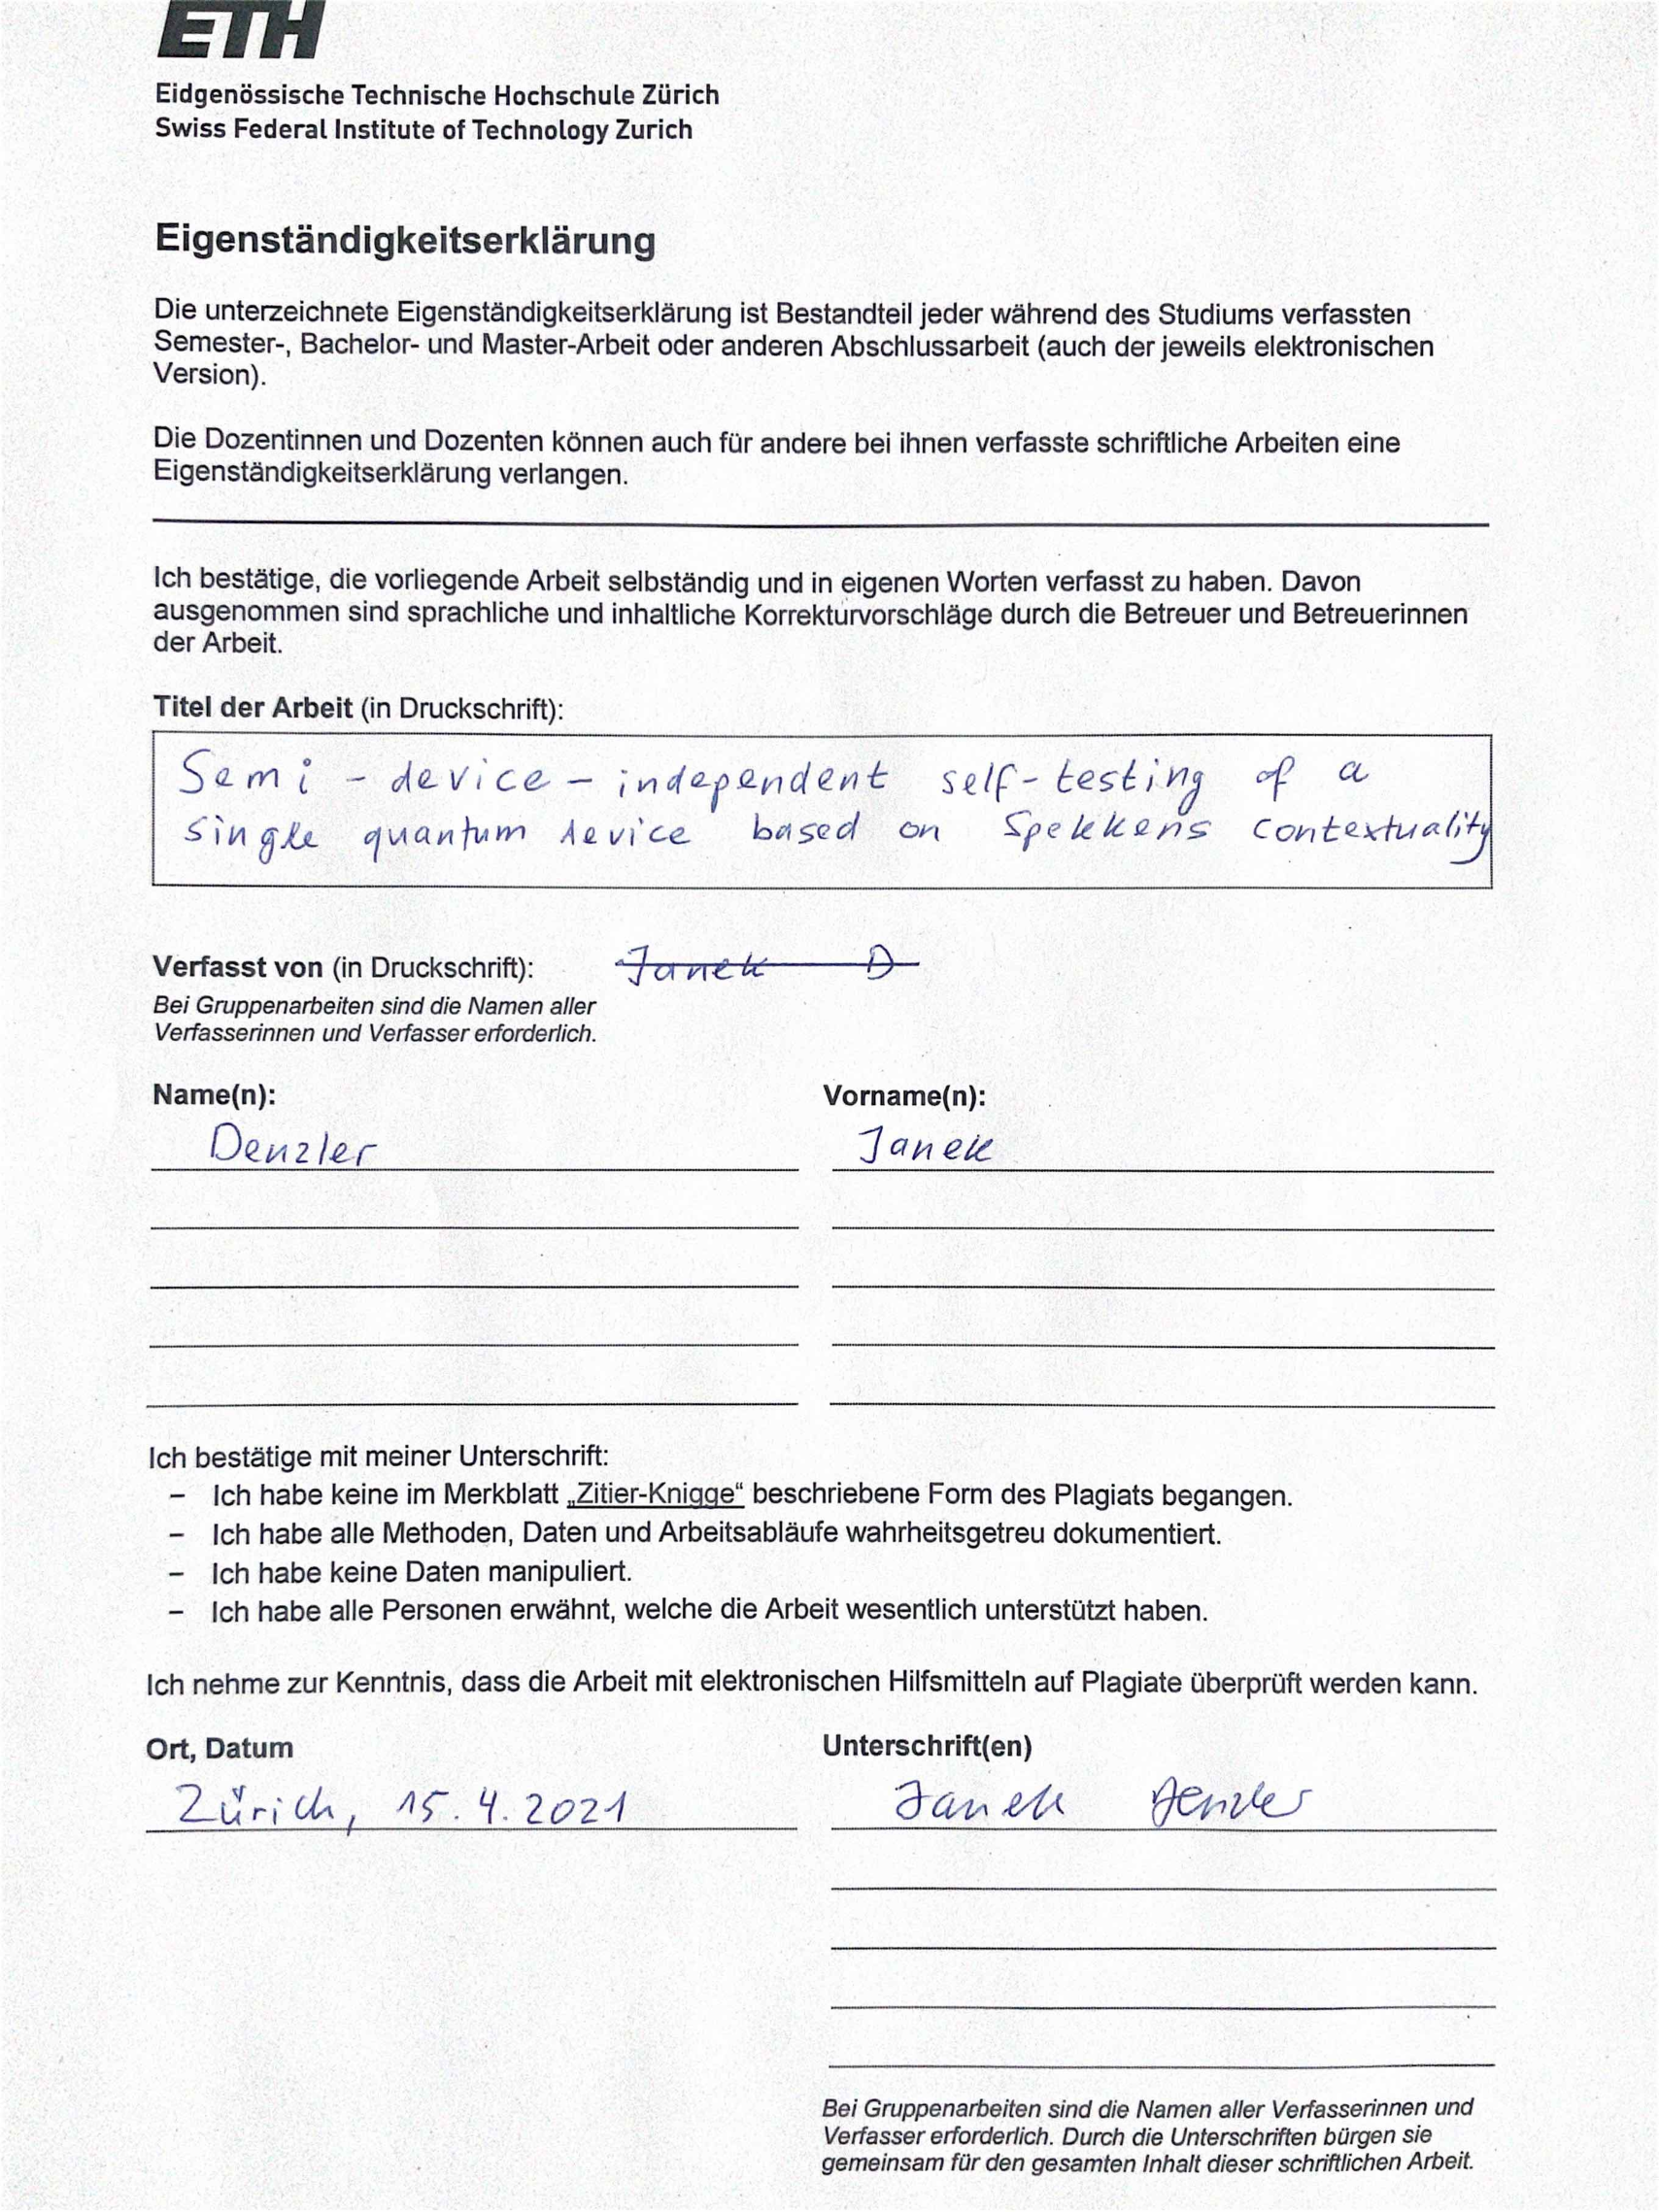
\includepdf[pages=-]{declaration-originality.pdf}
\end{document}  % The End
%% ----------------------------------------------------------------
